\documentclass[zavrsnirad]{fer}
% Dodaj opciju upload za generiranje konačne verzije koja se učitava na FERWeb

\usepackage{amsmath}
\usepackage{amssymb}
\usepackage{graphicx}
\usepackage{booktabs}
\usepackage{xcolor}
\usepackage{subcaption}
\usepackage{float}
\usepackage{placeins}
\usepackage{hyperref}
\usepackage{minted}

% Stil za sve code listinge (minted)
\setminted{
  fontsize=\footnotesize,
  linenos=true,
  frame=single,
  framesep=6pt,
  breaklines=true,
  style=tango,
}


%--- PODACI O RADU ----------------------------------------

\title{Mobile Robot Path Planning in a Known Environment Using Nonlinear Model Predictive Control}
\naslov{Planiranje putanje mobilnog robota u poznatom prostoru primjenom nelinearnog modelskog prediktivnog upravljanja}
\brojrada{2252}
\author{Luka Kordić}
\mentor{izv.~prof.~dr.~sc.~Branimir Novoselnik}
\date{June, 2026}
\datum{lipanj, 2026.}

%---------------------------------------------------------


\begin{document}

\maketitle

\zadatak{zadatak.pdf}

\begin{zahvale}
Zahvaljujem mentoru izv.~prof.~dr.~sc.~Branimiru Novoselnik na usmjeravanju, korisnim komentarima i strpljenju tijekom izrade ovog rada.
\end{zahvale}

\mainmatter

\tableofcontents


%--- POGLAVLJA -------------------------------------------

% !TEX root = ../zavrsni_rad.tex

\chapter{Uvod}
\label{pog:uvod}

\section{Motivacija i kontekst}

Robotski usisavači danas su jedan od najprodavanijih kućanskih uređaja s robotskom tehnologijom. Uređaji poput iRobot Roomba ili Ecovacs Deebot svakodnevno rješavaju zadatak autonomne navigacije u stambenom prostoru: kreću od baze za punjenje, pokrivaju čitavu površinu poda, izbjegavaju stolice, kućne ljubimce i stepenice, te se vraćaju na bazu kada završe ili im se isprazni baterija. Iza toga se, međutim, kriju dva klasična problema robotike: kako pronaći put od polazišta do cilja bez sudara s preprekama i kako robot stvarno prati taj put dovoljno precizno.

U ovom radu ta su dva problema riješena zajedno: izgrađen je sustav koji prvo planira put kroz prostor s preprekama, a zatim robot točno prati taj put. Koristi se model jednokolice --- jednostavan matematički opis kretanja robota koji dobro opisuje kako se kreće diferencijalno upravljani robot poput usisavača. Za razliku od problema poput uspravljanja njihala na kolicima gdje su sile i inercija neophodne za opis ponašanja sustava, istraživanjem je utvrđeno da za mobilnog robota koji se kreće po ravnoj podlozi pri malim brzinama takav model potpuno opisuje sve relevantne aspekte kretanja. Svi su eksperimenti provedeni u simulaciji u unaprijed poznatoj okolini.

\section{Pregled pristupa planiranju i regulaciji}

\subsection{Planiranje putanje}

Razvoj algoritama za planiranje putanje mobilnih robota proteže se kroz nekoliko desetljeća istraživanja. Najraniji pristupi temelje se na pretraživanju grafova u diskretiziranom prostoru. Dijkstrin algoritam garantira optimalnost ali ne koristi heurističku informaciju o cilju. \textbf{A* algoritam} \cite{astar}, uveden 1968.\ godine, dodaje procjenu preostale udaljenosti do cilja --- ravnu liniju do cilja --- i time značajno ubrzava pretraživanje uz zadržavanje optimalnosti. A* se danas smatra standardnim rješenjem za planiranje putanje u poznatim okolinama. Istraživanjem stvarnih robotskih sustava utvrđeno je da je A* široko zastupljen u praksi --- koristi se za planiranje putanje u ROS-u (\textit{Robot Operating System}), standardnoj platformi istraživačke robotike.

Algoritam je posebno dobro obrađen na kolegiju Uvod u umjetnu inteligenciju na FER-u, što je dodatno učvrstilo razumijevanje njegovih svojstava i olakšalo primjenu u ovom radu.


\subsection{Praćenje putanje}

Problem praćenja putanje na prvi pogled izgleda jednostavno --- robot treba slijediti zadanu liniju. No mobilni robot poput jednokolice ima jedno ključno ograničenje: može se kretati samo u smjeru u koji je okrenut, ne i bočno. To znači da robot ne može jednostavno "skliznuti" na putanju ako se od nje odmakne, nego mora okretanjem i vožnjom naprijed postupno korigirati svoju poziciju i orijentaciju. Uz to, robot ima fizikalna ograničenja --- maksimalnu brzinu, maksimalnu kutnu brzinu i ograničenja na to koliko brzo može mijenjati te veličine.

Za praćenje generirane putanje postoje razni pristupi --- geometrijski regulatori poput Pure Pursuit i Stanley regulatora \cite{siegwart_robotics}, PID regulatori i LQR. Svi su relativno jednostavni za implementaciju, ali zajednički im je nedostatak: ne gledaju unaprijed i ne uzimaju u obzir ograničenja sustava na formalan način.

\textbf{Modelsko prediktivno upravljanje} (MPC) \cite{rawlings_mpc} rješava upravo to: na svakom koraku gleda unaprijed kroz cijeli predikcijski horizont i optimizira upravljanje uz eksplicitno poštivanje svih ograničenja. \textbf{Nelinearno MPC} (NMPC) proširuje taj pristup na nelinearne sustave poput jednokolice. U ovom radu implementirano je korištenjem alata acados \cite{acados}.

\section{Doprinosi i opseg rada}

U ovom radu izgrađen je sustav koji kombinira A* algoritam za planiranje putanje s NMPC regulatorom za model jednokolice. Cilj je bio razumjeti kako takav sustav radi u praksi i izmjeriti koliko je dobar u različitim situacijama.

Konkretno, u radu je napravljeno:

\begin{enumerate}
  \item Prošireni model jednokolice u kojemu su promjene brzine upravljačke veličine, što olakšava postavljanje ograničenja u NMPC-u
  \item Meka ograničenja izbjegavanja prepreka koja sprječavaju koliziju ali ne uzrokuju neriješivost optimizacijskog problema
  \item Simulacijsko okruženje s testiranjem robustnosti na vanjske poremećaje i vizualizacijom rezultata
  \item Testiranje na sedam scenarija različite složenosti i analiza utjecaja ključnih parametara sustava
\end{enumerate}

% !TEX root = ../zavrsni_rad.tex

\chapter{Model mobilnog robota}
\label{pog:model}

\section{Kinematički model jednokolice}

Robot je modeliran kao jednokolica --- najjednostavniji model dvodimenzionalnog kretanja. Model koristi translacijsku brzinu $v$ i kutnu brzinu $\omega$ kao apstrakciju kretanja, što ga čini prikladnim za diferencijalno upravljane robote poput robotskog usisavača gdje se smjer kretanja postiže razlikom brzina dva kotača.
Stanje robota opisano je s pet veličina:

\begin{equation}
  \mathbf{x} = \begin{bmatrix} x \\ y \\ \theta \\ v \\ \omega \end{bmatrix}
\end{equation}

gdje su $x$ i $y$ koordinate robota u prostoru, $\theta$ kut orijentacije (mjeren od osi $x$, od $-\pi$ do $\pi$), $v$ translacijska brzina i $\omega$ kutna brzina.

Jednadžbe kretanja su:

\begin{equation}
  \dot{x} = v\cos\theta, \qquad \dot{y} = v\sin\theta, \qquad \dot{\theta} = \omega
\end{equation}

Ovo su standardne jednadžbe jednokolice. Robot se može kretati samo naprijed-nazad u smjeru u koji je okrenut --- ne može bočno. Zbog toga, ako se robot odmakne od referentne putanje, ne može jednostavno skliznuti natrag, nego mora okretanjem i vožnjom postupno korigirati poziciju i orijentaciju.

\section{Prošireni model s inkrementalnim upravljanjem}

U osnovnom modelu jednokolice upravljačke veličine su direktno brzine $v$ i $\omega$. Međutim, u praksi robot ne može trenutačno promijeniti brzinu --- postoje fizikalna ograničenja na to koliko brzo se brzina može mijenjati. Ako bismo ta ograničenja pokušali direktno implementirati u NMPC-u s $v$ i $\omega$ kao upravljanjem, formulacija postaje komplicirana.

Rješenje je jednostavno: umjesto da upravljamo direktno brzinama, upravljamo njihovim \textbf{promjenama} $\Delta v$ i $\Delta\omega$. Brzine $v$ i $\omega$ postaju dio vektora stanja, a upravljački vektor postaje:

\begin{equation}
  \mathbf{u} = \begin{bmatrix} \Delta v \\ \Delta\omega \end{bmatrix}
\end{equation}

Cijeli vektor stanja sada ima pet komponenti, a dinamika proširenog modela glasi:

\begin{equation}
  \dot{\mathbf{x}} = f(\mathbf{x}, \mathbf{u}) =
  \begin{bmatrix}
    v\cos\theta \\
    v\sin\theta \\
    \omega \\
    \Delta v \\
    \Delta\omega
  \end{bmatrix}
\end{equation}

Prednost ovog pristupa je što ograničenja na brzinu promjene postaju jednostavna intervalna ograničenja na upravljanje:

\begin{equation}
  |\Delta v| \leq 0{,}5 \ \text{m/s}^2, \qquad |\Delta\omega| \leq 1{,}0 \ \text{rad/s}^2
\end{equation}

A ograničenja na same iznose brzina postaju intervalna ograničenja na stanja:

\begin{equation}
  0{,}05 \leq v \leq 1{,}0 \ \text{m/s}, \qquad |\omega| \leq 1{,}5 \ \text{rad/s}
\end{equation}

Minimalna brzina $v_{min} = 0{,}05$ m/s osigurava da robot uvijek napreduje prema cilju --- bez te granice, optimizator bi u složenim situacijama mogao odabrati zaustavljanje kao lokalni optimum i robot bi zaostao iza referentne putanje koja kontinuirano napreduje.

Implementacija modela koristi CasADi --- biblioteku za simboličku matematiku. Umjesto računanja s konkretnim brojevima, CasADi radi sa simboličkim varijablama poput $x$, $\theta$, $v$ iz kojih automatski izvodi derivacije potrebne za optimizaciju. To znači da dinamički model trebamo napisati samo jednom, a acados iz njega sam generira optimizirani C kod solvera bez ručnog računanja Jacobijana. Alternativa bi bila ručno izvođenje parcijalnih derivacija, no CasADi taj postupak čini bržim i jednostavnijim za promjene modela.

\begin{listing}[H]
\begin{minted}{python}
model.x = ca.vertcat(x, y, theta, v, omega)
model.u = ca.vertcat(dv, domega)

model.f_expl_expr = ca.vertcat(
    v * ca.cos(theta),   # dx/dt
    v * ca.sin(theta),   # dy/dt
    omega,               # dtheta/dt
    dv,                  # dv/dt
    domega,              # domega/dt
)
\end{minted}
\caption{Implementacija proširenog modela jednokolice u \texttt{src/model.py}}
\end{listing}

\section{Numerička integracija — metoda Runge-Kutta 4. reda}

NMPC regulator interno rješava optimizacijski problem, ali nam je potrebna i odvojena numerička metoda za simulaciju "pravog robota" koji slijedi upravljačke naredbe. U tu svrhu koristi se metoda Runge-Kutta 4. reda (RK4).

RK4 aproksimira kretanje robota kroz jedan vremenski korak $\Delta t = 0{,}1$ s na sljedeći način:

\begin{equation}
  k_1 = f(\mathbf{x}_k, \mathbf{u}_k)
\end{equation}
\begin{equation}
  k_2 = f\!\left(\mathbf{x}_k + \tfrac{\Delta t}{2}k_1,\ \mathbf{u}_k\right)
\end{equation}
\begin{equation}
  k_3 = f\!\left(\mathbf{x}_k + \tfrac{\Delta t}{2}k_2,\ \mathbf{u}_k\right)
\end{equation}
\begin{equation}
  k_4 = f(\mathbf{x}_k + \Delta t\, k_3,\ \mathbf{u}_k)
\end{equation}
\begin{equation}
  \mathbf{x}_{k+1} = \mathbf{x}_k + \frac{\Delta t}{6}(k_1 + 2k_2 + 2k_3 + k_4)
\end{equation}

RK4 je odabran kao standardna metoda numeričke integracije koja se široko koristi u simulacijama dinamičkih sustava. Tijekom razvoja testirana je i Eulerova metoda, no rezultati su bili gotovo identični RK4-u, a ponekad s većim odstupanjima nego što bi teorija sugerirala. Iz tog razloga u konačnoj implementaciji zadržan je samo RK4. Implementacija u \texttt{src/simulation.py} direktno odgovara gornjim jednadžbama i koristi isti $f$ kao i model definiran u \texttt{src/model.py}, čime je osigurana konzistentnost između simulacije i predikcijskog modela u NMPC-u.

% !TEX root = ../zavrsni_rad.tex

\chapter{Nelinearno modelsko prediktivno upravljanje}
\label{pog:nmpc}

\section{Što je MPC}

MPC (eng.\ \textit{Model Predictive Control}) \cite{rawlings2017mpc, borrelli2017predictive} na svakom koraku predviđa ponašanje sustava za sljedećih $N$ koraka i odabire upravljanje koje minimizira grešku u tom budućem prozoru, uz poštivanje svih ograničenja.

Analogno iskusnom vozaču koji gleda cestu 20 metara unaprijed: ne samo da uočava ono što dolazi, nego već sada planira buduće kočenje ili skretanje da problem riješi prije nego se pojavi.

Konkretno, na svakom koraku:
\begin{enumerate}
  \item izmjeri se trenutno stanje robota $(x, y, \theta, v, \omega)$
  \item optimizira se upravljanje za sljedećih $N = 20$ koraka ($= 2$ sekunde unaprijed)
  \item primijeni se samo \textbf{prvi} upravljački signal iz tog plana
  \item ponovi se u sljedećem koraku s novim mjerenjem
\end{enumerate}

Ovaj pristup se naziva klizni horizont (eng.\ \textit{receding horizon}): horizont se stalno pomiče naprijed zajedno s robotom. Prednost je što svako novo mjerenje automatski ispravlja akumulirane greške ili vanjske poremećaje.

\begin{figure}[H]
  \centering
  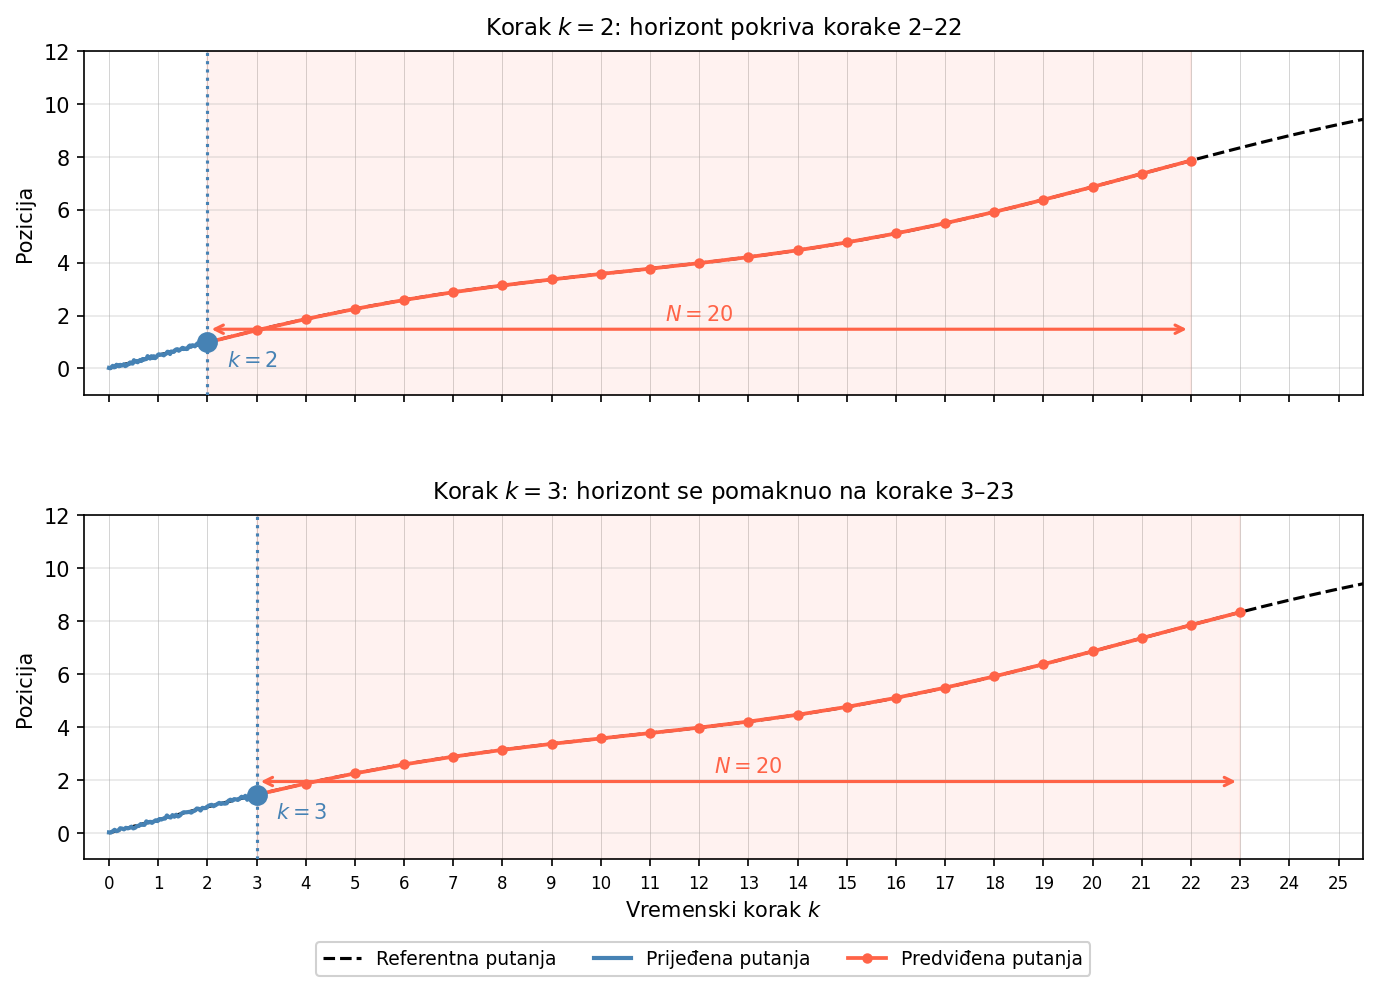
\includegraphics[width=0.95\linewidth]{figures/mpc_receding_horizon.png}
  \caption{Ilustracija kliznog horizonta. U koraku $k=2$ NMPC optimizira upravljanje za korake 2--22 (crveni segment, $N=20$). U sljedećem koraku $k=3$ horizont se pomiče naprijed na korake 3--23. Plava linija pokazuje prijeđenu putanju, a isprekidana crna referentnu.}
  \label{slk:receding_horizon}
\end{figure}

\textbf{Nelinearni MPC} (NMPC) je varijanta koja radi direktno s nelinearnim modelom. Jednokolica je nelinearna jer njezine jednadžbe kretanja sadrže $v\cos\theta$ i $v\sin\theta$ --- brzina i kut orijentacije su množeni, što sustav čini nelinearnim. Konkretno: robot koji vozi brzinom $v = 1$ m/s ravno ($\theta = 0$) kreće se isključivo u smjeru osi $x$, a isti robot koji vozi istom brzinom ali okrenut za $\theta = \pi/2$ kreće se isključivo u smjeru osi $y$ --- isti ulaz, potpuno drugačiji efekt ovisno o trenutnom stanju. Da je sustav linearan, način na koji upravljanje utječe na promjenu stanja bio bi konstantan i neovisan o trenutnoj orijentaciji. U monociklu naprotiv, faktori $\cos\theta$ i $\sin\theta$ množe brzinu $v$ --- isti upravljački signal pri različitom $\theta$ daje potpuno drugačiji smjer promjene pozicije. Zbog toga je potreban nelinearni optimizacijski pristup poput SQP-a.

\begin{figure}[H]
  \centering
  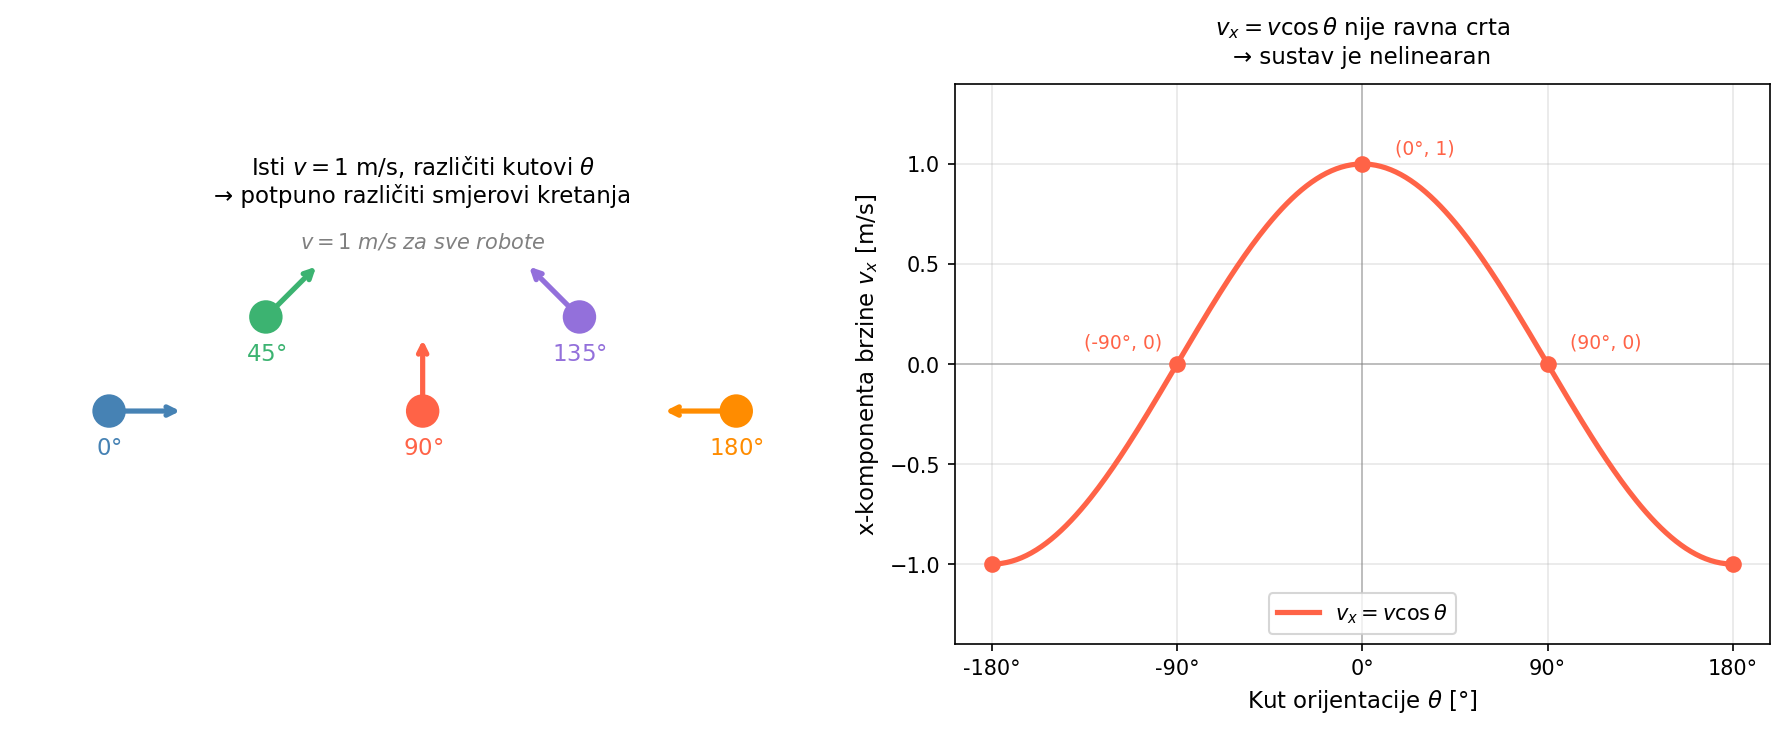
\includegraphics[width=0.95\linewidth]{figures/unicycle_nonlinear.png}
  \caption{Lijevo: robot pri istoj brzini $v=1$ m/s ali različitim kutovima orijentacije --- smjer kretanja potpuno se mijenja ovisno o stanju. Desno: x-komponenta brzine $v_x = v\cos\theta$ u ovisnosti o kutu --- valovita krivulja, ne ravna crta, što znači da je sustav nelinearan.}
  \label{slk:unicycle_nonlinear}
\end{figure}

\section{Formulacija optimizacijskog problema}

Cijeli NMPC problem može se zapisati kao optimizacijski problem s ograničenjima (OCP, eng.\ \textit{Optimal Control Problem}):

\begin{equation}
\label{eq:ocp}
\begin{aligned}
\min_{\substack{\mathbf{u}_0,\ldots,\mathbf{u}_{N-1} \\ \mathbf{s}_{0},\ldots,\mathbf{s}_{N-1}}} \quad
  & \sum_{k=0}^{N-1} \bigl\|\mathbf{y}_k - \mathbf{y}_{ref,k}\bigr\|^2_{W}
    + \bigl\|\mathbf{y}_N - \mathbf{y}_{ref,N}\bigr\|^2_{W_e}
    + \sum_{k=0}^{N-1} \sum_i \bigl( w_L\, s_{i,k} + w_Q\, s_{i,k}^2 \bigr) \\
\text{uz uvjet} \quad
  & \mathbf{x}_{k+1} = \Phi(\mathbf{x}_k, \mathbf{u}_k), \quad k = 0,\ldots,N-1 \\
  & \mathbf{x}_0 = \mathbf{x}_{meas} \\
  & |a_{v,k}| \leq 0{,}5 \ \text{m/s}^2, \quad |\alpha_k| \leq 1{,}0 \ \text{rad/s}^2 \\
  & 0{,}05 \leq v_k \leq 1{,}0 \ \text{m/s}, \quad |\omega_k| \leq 1{,}5 \ \text{rad/s} \\
  & h_i(\mathbf{x}_k) + s_{i,k} \geq 0, \quad s_{i,k} \geq 0
\end{aligned}
\end{equation}

gdje $\Phi(\mathbf{x}_k, \mathbf{u}_k)$ označava numerički integrator dinamike s korakom $\Delta t = 0{,}1$ s (konkretno ERK4 (eng.\ \textit{Explicit Runge-Kutta}, ERK) --- eksplicitna Runge-Kutta metoda 4.\ reda), $h_i(\mathbf{x}) = \|\mathbf{p} - \mathbf{c}_i\|_2 - r_i$ je udaljenost centra robota $\mathbf{p} = (x, y)$ od granice prepreke $i$ (centar $\mathbf{c}_i$, polumjer $r_i$), a $s_{i,k} \geq 0$ su slack varijable koje dopuštaju meka kršenja ograničenja prepreka uz kaznu $w_L = w_Q = 10^4$.

Sljedeće sekcije opisuju detaljno svaki od sastavnih dijelova ovog problema.

\section{Funkcija troška}

Na svakom koraku NMPC traži upravljačku sekvencu $\mathbf{u}_0, \ldots, \mathbf{u}_{N-1}$ koja minimizira kvadratnu funkciju troška:

\begin{equation}
  \min_{\mathbf{u}_0,\, \ldots,\, \mathbf{u}_{N-1}} \sum_{k=0}^{N-1} \|\mathbf{y}_k - \mathbf{y}_{ref,k}\|^2_W + \|\mathbf{y}_N - \mathbf{y}_{ref,N}\|^2_{W_e}
\end{equation}

gdje je $\mathbf{y}_k$ izlazni vektor koji kombinira stanja i upravljanje, a $\mathbf{y}_{ref,k}$ referentni vektor koji dolazi s A* putanje:

\begin{equation}
  \mathbf{y}_k = \begin{bmatrix} x_k \\ y_k \\ \theta_k \\ a_{v,k} \\ \alpha_k \end{bmatrix}, \qquad
  \mathbf{y}_{ref,k} = \begin{bmatrix} x_{ref} \\ y_{ref} \\ \theta_{ref} \\ 0 \\ 0 \end{bmatrix}
\end{equation}

Nule na kraju $\mathbf{y}_{ref,k}$ znače da su željena ubrzanja nula --- robot treba mijenjati brzinu samo koliko je nužno za praćenje putanje. Matrica troška $W$ blok-dijagonalne je strukture:

\begin{equation}
  W = \begin{bmatrix} Q & 0 \\ 0 & R \end{bmatrix}, \qquad
  Q = \begin{bmatrix} 10{,}0 & 0 & 0 \\ 0 & 10{,}0 & 0 \\ 0 & 0 & 1{,}0 \end{bmatrix}, \qquad
  R = \begin{bmatrix} 0{,}1 & 0 \\ 0 & 0{,}1 \end{bmatrix}
\end{equation}

Omjer dijagonalnih elemenata $Q_{xx} / R_{a_v} = 10{,}0 / 0{,}1 = 100$ znači da je korekcija pozicije 100 puta važnija od glatkoće upravljanja. Terminalna matrica $W_e = Q$ kažnjava grešku na kraju horizonta istim težinama --- odabir $W_e = Q$ je heuristički i u praksi se pokazao stabilnim, no postoje i sofisticiranije metode (npr.\ rješavanje Riccatijeve jednadžbe).

Ove vrijednosti nisu odabrane nasumično --- u poglavlju~\ref{pog:rezultati} prikazana je analiza kako različiti omjeri $Q/R$ utječu na preciznost praćenja.

Izlazni vektor $\mathbf{y}_k$ dobiva se linearnom projekcijom stanja i upravljanja: $\mathbf{y}_k = V_x \mathbf{x}_k + V_u \mathbf{u}_k$, gdje su projekcijske matrice:

\begin{equation}
  V_x = \begin{bmatrix}
    1 & 0 & 0 & 0 & 0 \\
    0 & 1 & 0 & 0 & 0 \\
    0 & 0 & 1 & 0 & 0 \\
    0 & 0 & 0 & 0 & 0 \\
    0 & 0 & 0 & 0 & 0
  \end{bmatrix}, \qquad
  V_u = \begin{bmatrix}
    0 & 0 \\
    0 & 0 \\
    0 & 0 \\
    1 & 0 \\
    0 & 1
  \end{bmatrix}
\end{equation}

Gornje tri komponente izlaza ($x$, $y$, $\theta$) dolaze iz vektora stanja, a donje dvije ($a_v$, $\alpha$) iz vektora upravljanja. Odgovarajuća implementacija u acadosu:

\begin{listing}[H]
\begin{minted}{python}
Q = np.diag(mpc["Q"])   # diag(10, 10, 1) -- x, y, theta
R = np.diag(mpc["R"])   # diag(0.1, 0.1)  -- dv, domega

ocp.cost.Vx = np.zeros((ny, nx))
ocp.cost.Vx[:3, :3] = np.eye(3)    # uzmi x, y, theta iz stanja

ocp.cost.Vu = np.zeros((ny, nu))
ocp.cost.Vu[3:, :] = np.eye(nu)    # uzmi dv, domega iz upravljanja

ocp.cost.W   = np.block([[Q, np.zeros((3, nu))],
                          [np.zeros((nu, 3)), R]])
ocp.cost.W_e = Q                    # terminalna matrica = Q
\end{minted}
\caption{Postavljanje matrica troška u \texttt{src/mpc\_solver.py}}
\end{listing}

\section{Ograničenja}

Sva fizikalna ograničenja robota direktno su ugrađena u optimizacijski problem. Ograničenja na upravljanje (maksimalna ubrzanja):

\begin{equation}
  |a_v| \leq 0{,}5 \ \text{m/s}^2, \qquad |\alpha| \leq 1{,}0 \ \text{rad/s}^2
\end{equation}

Ograničenja na stanja (fizikalne granice robota i okolina):

\begin{equation}
  0{,}05 \leq v \leq 1{,}0 \ \text{m/s}, \qquad |\omega| \leq 1{,}5 \ \text{rad/s}
\end{equation}
\begin{equation}
  0 \leq x \leq 10 \ \text{m}, \qquad 0 \leq y \leq 10 \ \text{m}
\end{equation}

Implementacija u \texttt{src/mpc\_solver.py}:

\begin{listing}[H]
\begin{minted}{python}
ocp.constraints.lbu = np.array([-robot["dv_max"], -robot["domega_max"]])  # dv, domega min
ocp.constraints.ubu = np.array([ robot["dv_max"],  robot["domega_max"]])  # dv, domega max

ocp.constraints.lbx = np.array([env["x_min"], env["y_min"], -np.pi,
                                 robot["v_min"], -robot["omega_max"]])     # donje granice stanja
ocp.constraints.ubx = np.array([env["x_max"], env["y_max"],  np.pi,
                                 robot["v_max"],  robot["omega_max"]])     # gornje granice stanja
\end{minted}
\caption{Postavljanje ograničenja u \texttt{src/mpc\_solver.py}}
\end{listing}

\section{Meka ograničenja izbjegavanja prepreka}

Za svaku kružnu prepreku s centrom $(c_x, c_y)$ i polumjerom $r$ definira se uvjet sigurnosne udaljenosti:

\begin{equation}
  h(\mathbf{x}) = (x - c_x)^2 + (y - c_y)^2 - (r + r_{rob})^2 \geq 0
\end{equation}

gdje je $r_{rob} = 0{,}2$ m polumjer robota. Ovaj uvjet mora biti zadovoljen za svaki korak horizonta.

Ograničenja su implementirana kao \textbf{meka} (eng.\ \textit{soft}): umjesto da se zahtijeva $h_i(\mathbf{x}_k) \geq 0$, uvodi se slack varijabla $s_{i,k} \geq 0$ i relaksirani uvjet postaje:

\begin{equation}
  h_i(\mathbf{x}_k) + s_{i,k} \geq 0, \qquad s_{i,k} \geq 0
\end{equation}

Kada je $s_{i,k} = 0$, ograničenje je zadovoljeno; kada je $s_{i,k} > 0$, robot je unutar sigurnosne zone prepreke $i$ i veličina $s_{i,k}$ mjeri iznos kršenja. Svaka slack varijabla kažnjava se u funkciji troška linearnim i kvadratnim penalom:

\begin{equation}
  \sum_{k=0}^{N-1} \sum_i \bigl( w_L\, s_{i,k} + w_Q\, s_{i,k}^2 \bigr), \qquad w_L = w_Q = 10^4
\end{equation}

Linearna komponenta pokreće robot iz prepreke čak i kod malih kršenja, a kvadratna brzo raste s većim kršenjima. Meka formulacija korisna je jer održava numeričku rješivost OCP-a u uskim prostorima i pri nesavršenim referencama --- tvrda ograničenja bi u takvim situacijama uzrokovala neriješivost solvera.

\begin{listing}[H]
\begin{minted}{python}
for (cx, cy, r) in obstacles:
    # h(x) = (x-cx)^2 + (y-cy)^2 - (r + r_robot)^2 >= 0
    h_list.append((px - cx)**2 + (py - cy)**2 - (r + r_robot)**2)

ocp.model.con_h_expr = ca.vertcat(*h_list)   # nelinearna ograničenja za acados

penalty = 1e4                                  # kazna za kršenje ograničenja
ocp.cost.zl = penalty * np.ones(n_obs)        # linearni penalty
ocp.cost.Zl = penalty * np.ones(n_obs)        # kvadratni penalty
\end{minted}
\caption{Implementacija mekih ograničenja prepreka u \texttt{src/mpc\_solver.py}}
\end{listing}

\section{SQP\_RTI solver}

Za rješavanje nelinearnog optimizacijskog problema na svakom koraku koristi se SQP\_RTI (eng.\ \textit{Sequential Quadratic Programming --- Real-Time Iteration}) pristup unutar alata acados \cite{verschueren2022acados, acados_docs, diehl2002rti}.

SQP (eng.\ \textit{Sequential Quadratic Programming}) je metoda optimizacije koja iterativno linearizira nelinearni problem i rješava niz kvadratičnih potprograma. SQP\_RTI (eng.\ \textit{Real-Time Iteration}) je varijanta prilagođena za primjene u stvarnom vremenu i sastoji se od dvije faze koje se izmjenjuju u svakom regulacijskom koraku \cite{diehl2002rti}:

\begin{enumerate}
  \item \textbf{Faza pripreme} (eng.\ \textit{preparation phase}): linearizacija dinamike duž trenutne trajektorije, izračun Jacobijana, kondenzacija kvadratičnog potprograma (eng.\ \textit{Quadratic Program}, QP) --- ove operacije odvijaju se \textit{unaprijed}, dok robot još izvršava prethodni upravljački signal.
  \item \textbf{Faza povratne veze} (eng.\ \textit{feedback phase}): čim stigne novo mjerenje $\mathbf{x}_{meas}$, postavi se inicijalni uvjet i izvrši jedna SQP iteracija rješavanjem pripremljenog QP-a. Rezultat je novi upravljački signal koji se odmah šalje robotu.
\end{enumerate}

Zahvaljujući ovoj podjeli, kašnjenje između mjerenja i primjene upravljanja iznosi samo trajanje feedback faze (najmanji dio ukupnog računanja), dok se skuplja priprema odvija paralelno s izvođenjem prethodnog koraka.

Za rješavanje kvadratičnog potprograma unutar svake SQP iteracije koristi se HPIPM rješavač (eng.\ \textit{High Performance Interior Point Method}) koji je optimiziran za strukturu MPC problema. Gauss-Newtonova aproksimacija hesijana zamjenjuje pravi hesijan Lagrangiana aproksimacijom $J^\top W J$, gdje je $J$ Jacobijan reziduala (razlika $\mathbf{y}_k - \mathbf{y}_{ref,k}$) kvadratne funkcije troška, a $W$ težinska matrica. Time se izbjegava skupo računanje drugih derivacija nelinearne dinamike i ograničenja uz cijenu blago slabije konvergencije --- za RTI shemu s jednom iteracijom po koraku to je prihvatljiv kompromis.

Ukupno vrijeme rješavanja po koraku izmjereno u eksperimentima iznosi između $0{,}09$ i $0{,}12$ ms --- daleko ispod vremenskog koraka od $100$ ms, što ostavlja dovoljno prostora za opterećenje komunikacije i perifernih operacija.

\begin{listing}[H]
\begin{minted}{python}
ocp.solver_options.nlp_solver_type = mpc["solver_type"]   # "SQP_RTI"
ocp.solver_options.qp_solver       = "PARTIAL_CONDENSING_HPIPM"
ocp.solver_options.hessian_approx  = "GAUSS_NEWTON"
ocp.solver_options.integrator_type = "ERK"                # eksplicitni Runge-Kutta 4. reda
ocp.solver_options.nlp_solver_max_iter = 50
\end{minted}
\caption{Konfiguracija SQP\_RTI solvera u \texttt{src/mpc\_solver.py}}
\end{listing}

% !TEX root = ../zavrsni_rad.tex

\chapter{Globalno planiranje putanje}
\label{pog:astar}

\section{A* algoritam}

Prije nego NMPC može pratiti putanju, potrebno je tu putanju pronaći. A* algoritam pretražuje diskretiziranu mrežu prostora i pronalazi najkraći slobodan put od starta do cilja.

\subsection{Diskretizacija prostora}

Okolina dimenzija $10 \times 10$ m podijeli se u pravokutnu mrežu s rezolucijom $\delta = 0{,}2$ m po ćeliji, što daje mrežu $51 \times 51 = 2601$ čvorova. Svaka ćelija označena je kao slobodna ili blokirana na osnovu udaljenosti od prepreka:

\begin{equation}
  \text{blokirana}(i,j) = \left\| w_{i,j} - c_k \right\|_2 \leq r_k + r_{rob} + \delta_{inf}
\end{equation}

gdje je $w_{i,j}$ koordinata ćelije u prostoru, $c_k$ centar prepreke, $r_k$ njezin polumjer, $r_{rob} = 0{,}2$ m polumjer robota i $\delta_{inf} = 0{,}2$ m dodatno proširenje prepreke. Ukupno proširenje prepreke iznosi $r_{rob} + \delta_{inf} = 0{,}4$ m --- to znači da se centar robota ne može naći unutar 0,4 m od ruba bilo koje prepreke.

Implementacija u \texttt{src/astar.py}:

\begin{listing}[H]
\begin{minted}{python}
# ukupno proširenje = sigurnosna margina + polumjer robota
inflation = p["astar"]["obstacle_inflation"] + p["robot"]["radius"]  # 0.2 + 0.2 = 0.4 m

for (cx, cy, r) in to_acados_list(obstacles):  # za svaku prepreku (centar + polumjer)
    for i in range(nx):
        for j in range(ny):
            wx, wy = grid_to_world(i, j)        # indeks ćelije → koordinata u prostoru
            # ćelija je blokirana ako joj je centar unutar proširene prepreke
            if (wx - cx)**2 + (wy - cy)**2 <= (r + inflation)**2:
                occupied[i, j] = True
\end{minted}
\caption{Označavanje blokiranih ćelija u \texttt{src/astar.py}}
\end{listing}

\begin{figure}[H]
  \centering
  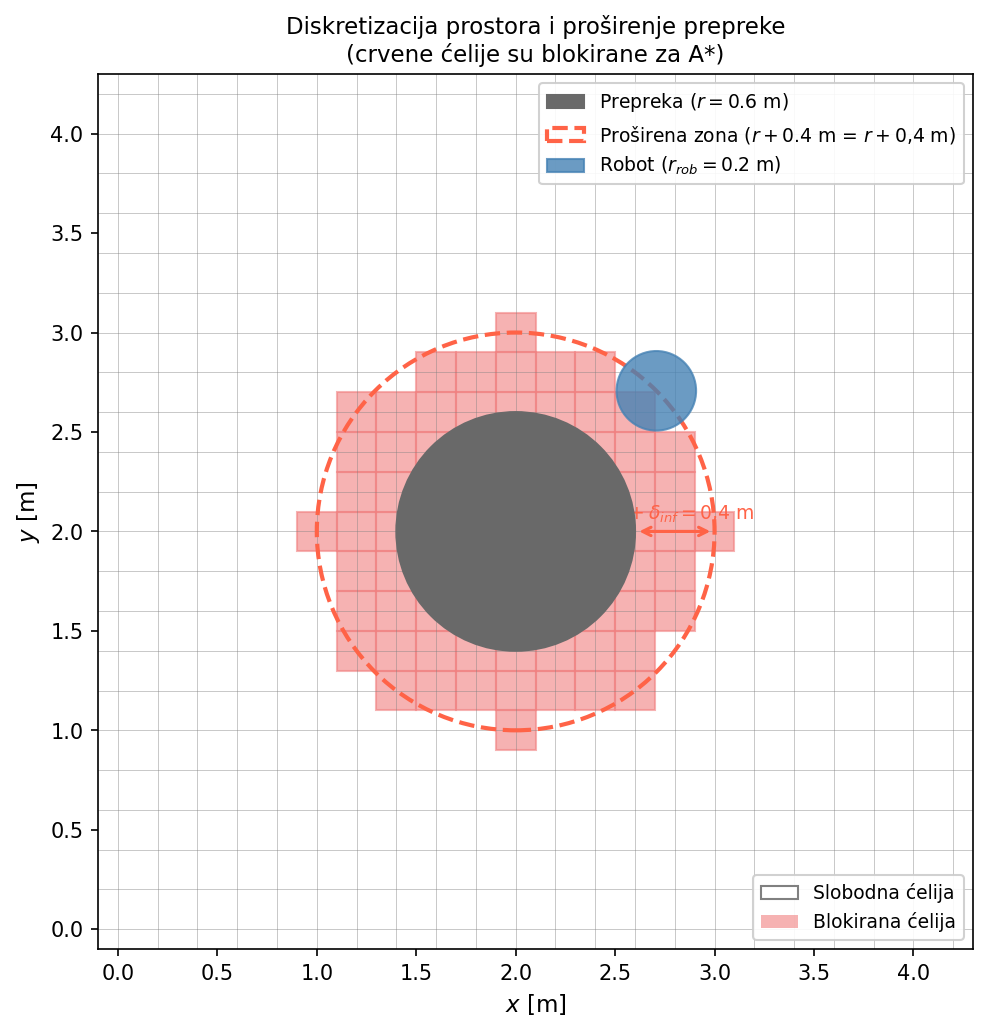
\includegraphics[width=0.75\linewidth]{figures/astar_grid.png}
  \caption{Diskretizacija prostora i proširenje prepreke. Crvene ćelije su blokirane za A* jer im je centar unutar proširene zone (isprekidani krug). Robot (plavi krug) može se kretati samo centrom slobodnih ćelija, što garantira da nikada neće doći u fizički kontakt s preprekom.}
  \label{slk:astar_grid}
\end{figure}

\subsection{Pretraga}

A* koristi prioritetni red i za svaki čvor $n$ prati procjenu ukupnog troška:

\begin{equation}
  f(n) = g(n) + h(n)
\end{equation}

gdje je $g(n)$ stvarni trošak puta od starta do čvora $n$, a $h(n)$ euklidska udaljenost do cilja:

\begin{equation}
  h(n) = \sqrt{(n_x - g_x)^2 + (n_y - g_y)^2}
\end{equation}

Algoritam uvijek proširuje čvor s najmanjim $f(n)$. Euklidska heuristika nikad ne precjenjuje stvarni trošak, što garantira pronalazak optimalnog puta. Susjedi se razmatraju u 8 smjerova --- 4 kardinalna (trošak 1,0) i 4 dijagonalna (trošak $\sqrt{2}$).

Kada A* prođe kroz sve dostupne ćelije i ne pronađe put do cilja, program javlja grešku --- to znači da put ne postoji:

\begin{listing}[H]
\begin{minted}{python}
neighbours = [(-1,0),(1,0),(0,-1),(0,1),       # kardinalni smjerovi
              (-1,-1),(-1,1),(1,-1),(1,1)]       # dijagonalni smjerovi

while open_set:
    _, g, current = heapq.heappop(open_set)     # uzmi čvor s najmanjim f
    if current == goal_g:
        # rekonstruiraj put unatrag
        ...
    for di, dj in neighbours:
        step = np.hypot(di, dj)                 # 1.0 ili sqrt(2)
        new_g = g + step
        if new_g < g_score.get(nb, np.inf):
            f = new_g + heuristic(nb, goal_g)
            heapq.heappush(open_set, (f, new_g, nb))

raise RuntimeError("A*: nema puta od starta do cilja")
\end{minted}
\caption{Jezgra A* pretrage u \texttt{src/astar.py}}
\end{listing}

\begin{figure}[H]
  \centering
  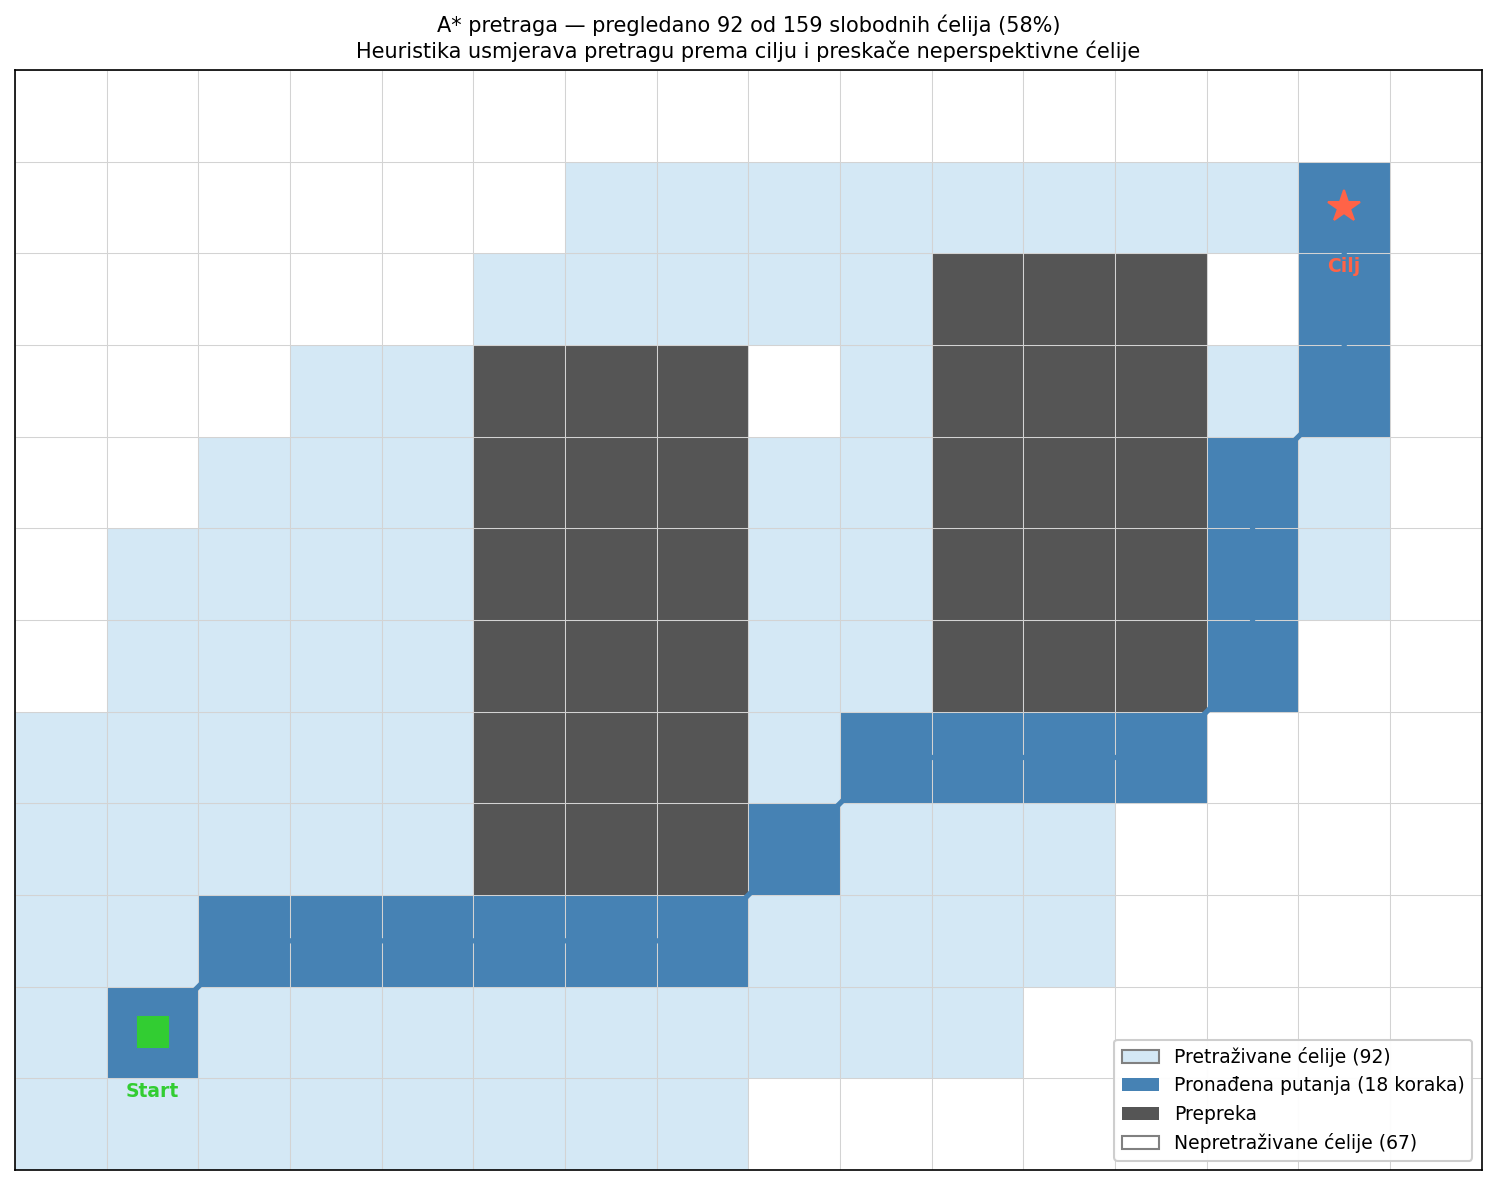
\includegraphics[width=0.90\linewidth]{figures/astar_search.png}
  \caption{Vizualizacija A* pretrage na primjeru mreže s dvije prepreke. Svjetloplavi čvorovi su pretraživani, tamno plavi čvorovi su na pronađenoj putanji, bijeli čvorovi nisu ni razmatrani. Heuristika usmjerava pretragu prema cilju i preskače neperspektivne čvorove.}
  \label{slk:astar_search}
\end{figure}

\subsection{Pravokutne prepreke}

A* radi s kružnim preprekama jer za njih proširenje prepreke ima jasnu geometrijsku interpretaciju. Pravokutne prepreke (korištene u L-hodniku i U-obliku) aproksimiraju se mrežom malih kružnica polumjera 0,2 m, što je razlog opisan u poglavlju~\ref{pog:nmpc} --- acados zahtijeva glatke, derivabilne funkcije za računanje Jacobijana.

\begin{listing}[H]
\begin{minted}{python}
def to_circles(self, r: float = 0.2) -> list[Circle]:
    circles = []
    x = self.x_min + r             # počni od lijevog ruba + polumjer
    while x <= self.x_max:
        y = self.y_min + r         # počni od donjeg ruba + polumjer
        while y <= self.y_max:
            circles.append(Circle(x, y, r))  # dodaj kružnicu u točki (x, y)
            y += r * 1.5           # razmak između kružnica (dovoljno gusto da nema prolaza)
        x += r * 1.5
    return circles
\end{minted}
\caption{Aproksimacija pravokutnika mrežom kružnica u \texttt{src/obstacles.py}}
\end{listing}

\begin{figure}[H]
  \centering
  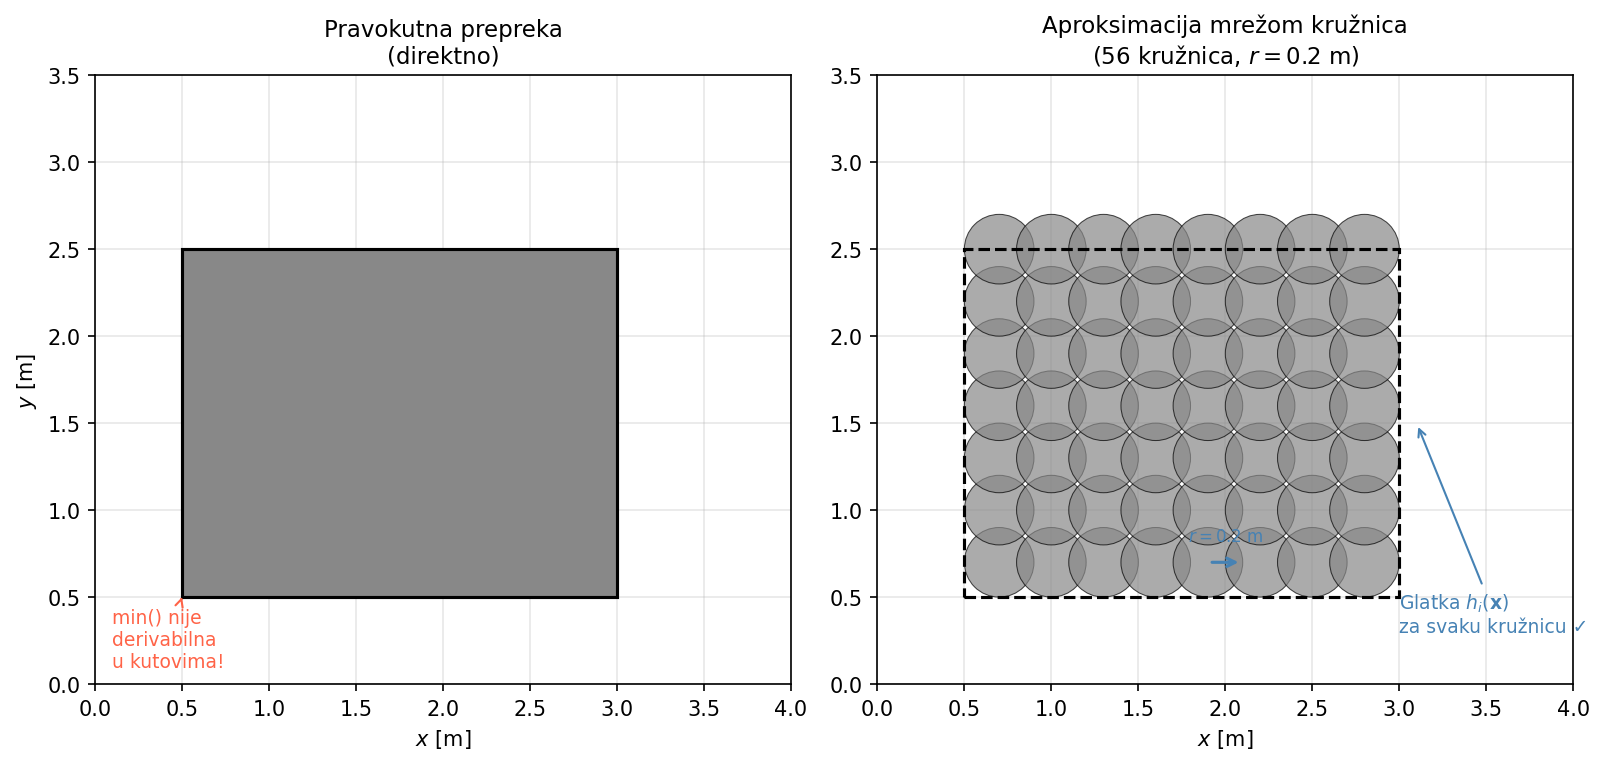
\includegraphics[width=0.95\linewidth]{figures/rect_to_circles.png}
  \caption{Lijevo: pravokutna prepreka direktno --- ograničenje $h(\mathbf{x})$ nije glatko u kutovima pa acados ne može računati Jacobijane. Desno: ista prepreka aproksimirana mrežom kružnica --- svaka kružnica ima glatku $h_i(\mathbf{x})$ pa SQP iteracije rade ispravno.}
  \label{slk:rect_to_circles}
\end{figure}

\section{Izglađivanje putanje}

A* putanja sadrži oštre kutove jer je ograničena rešetkom. Takva putanja nije pogodna kao referenca za NMPC jer zahtijeva nagle promjene smjera. Stoga se izglađuje \textbf{kubičnim B-splineom} koristeći \texttt{scipy.interpolate.splprep}:

\begin{listing}[H]
\begin{minted}{python}
tck, _ = splprep([pts[:, 0], pts[:, 1]], s=0.5, k=3)  # kubični spline, s=0.5
t = np.linspace(0, 1, n_points)                        # 200 jednakomjernih točaka
x_s, y_s = splev(t, tck)
\end{minted}
\caption{Izglađivanje putanje kubičnim splineom u \texttt{src/path\_smoother.py}}
\end{listing}

Parametar izglađivanja $s = 0{,}5$ dopušta B-spline krivulji da ne prolazi točno kroz sve A* točke, nego pronalazi glađu krivu koja eliminira sitne oscilacije rešetke. Rezultat je 200 ravnomjerno raspoređenih točaka duž glatke krivulje.

\begin{figure}[H]
  \centering
  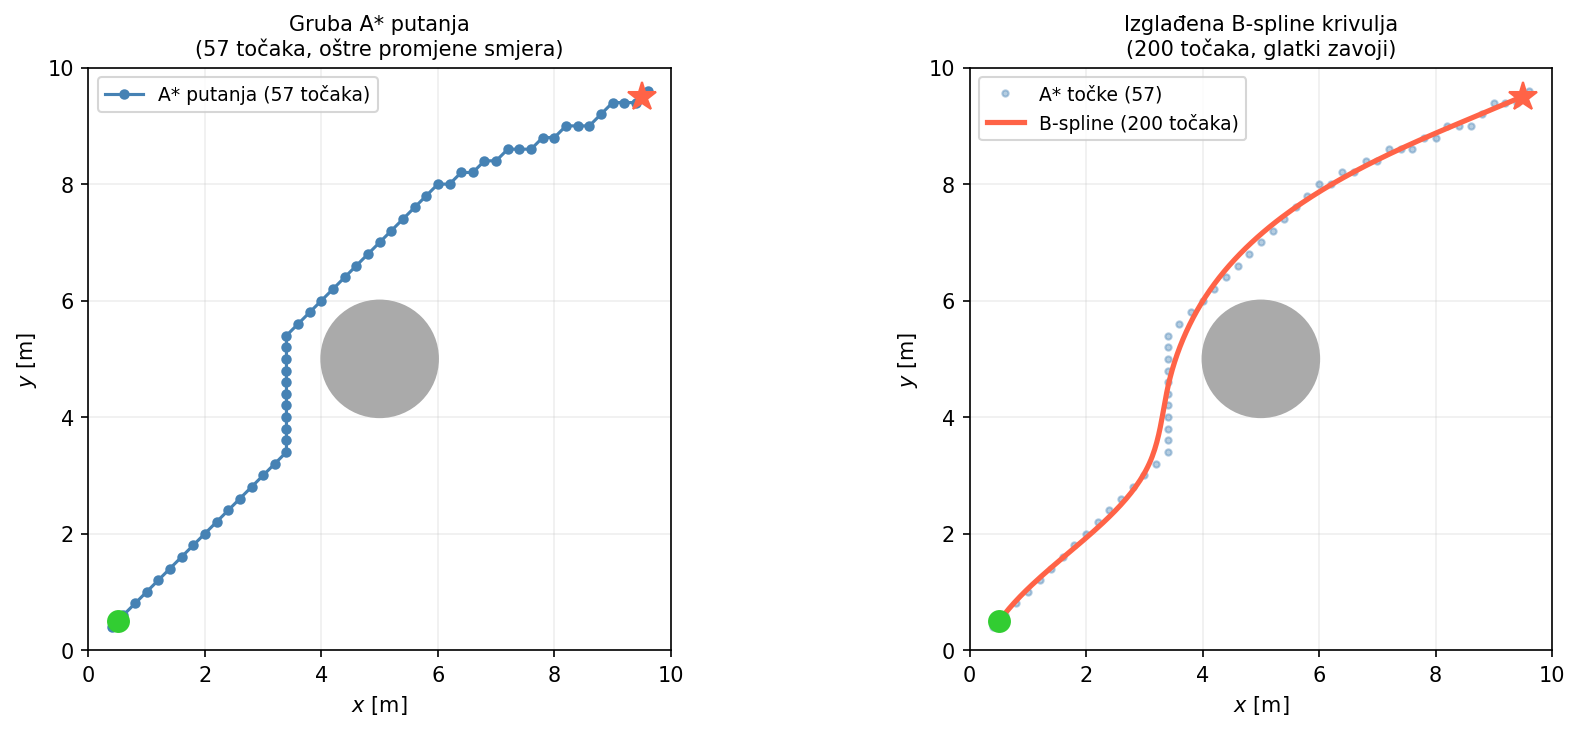
\includegraphics[width=0.95\linewidth]{figures/path_smoothing.png}
  \caption{Lijevo: gruba A* putanja s 57 točaka --- vidljive su oštre promjene smjera karakteristične za rešetku. Desno: ista putanja izglađena B-spline krivuljom s 200 ravnomjerno raspoređenih točaka. Scenarij \texttt{one\_obstacle}, generiran stvarnim kodom iz \texttt{src/astar.py} i \texttt{src/path\_smoother.py}.}
  \label{slk:path_smoothing}
\end{figure}

\section{Profil brzine}

Na ravnim dionicama robot vozi punom brzinom $v_{max} = 1{,}0$ m/s. U zavojima je poželjno usporiti kako bi se smanjila bočna greška praćenja. Referentna brzina računa se iz zakrivljenosti $\kappa$ putanje:

\begin{equation}
  v_{ref}(s) = \frac{v_{max}}{1 + k_{curv} \cdot \kappa(s)}, \qquad k_{curv} = 0{,}5
\end{equation}

gdje se zakrivljenost aproksimira vektorskim produktom uzastopnih segmenata putanje. Profil brzine koristi se isključivo za vizualizaciju referentnog signala u grafovima --- NMPC sam optimizira stvarnu brzinu unutar zadanih ograničenja.

\begin{figure}[H]
  \centering
  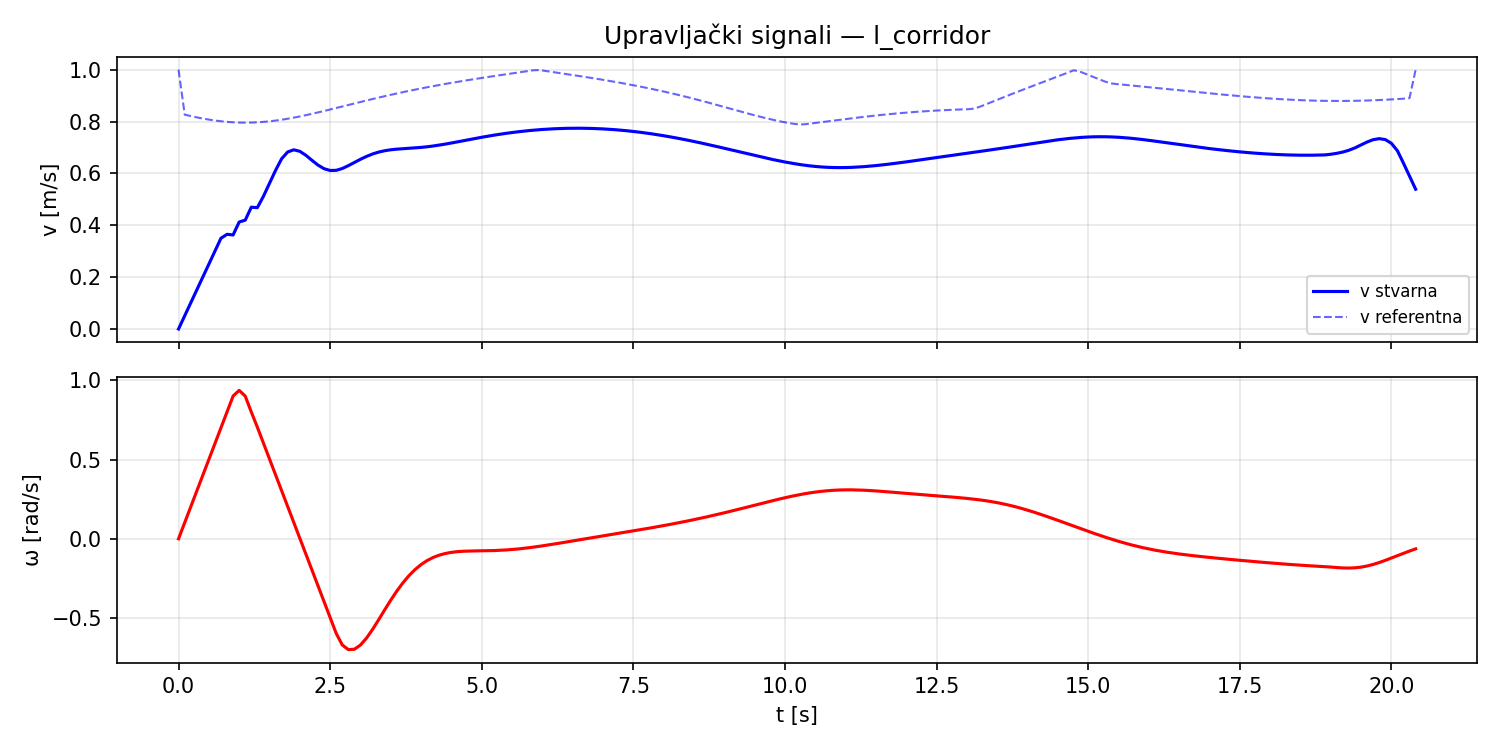
\includegraphics[width=0.90\linewidth]{figures/l_corridor_controls.png}
  \caption{Profil brzine u scenariju L-hodnika. Isprekidana linija prikazuje referentnu brzinu $v_{ref}$ izračunatu prema zakrivljenosti putanje --- vidljivi su padovi na zavojima. Puna linija prikazuje stvarnu brzinu koju NMPC optimizira neovisno o $v_{ref}$.}
  \label{slk:velocity_profile}
\end{figure}

% !TEX root = ../zavrsni_rad.tex

\chapter{Implementacija sustava}
\label{pog:implementacija}

\section{Arhitektura sustava}

Sustav je implementiran u Pythonu i organiziran u module koji odgovaraju logičkim slojevima arhitekture. Svaki modul ima jasno definiran ulaz i izlaz bez globalnog stanja. Sve konfiguracijske vrijednosti --- dimenzije okoline, parametri robota, horizonti i težine MPC-a --- čitaju se iz jedne datoteke \texttt{config/params.yaml}, čime je odvojena konfiguracija od logike.

Izvršavanje počinje u \texttt{src/scenarios.py}, koji za odabrani scenarij vraća rječnik s početnim stanjem robota, koordinatama cilja i popisom prepreka. Prepreke su definirane u \texttt{src/obstacles.py} kao instance klasa \texttt{Circle} i \texttt{Rectangle}. Pravokutne prepreke se interno aproksimiraju mrežom malih kružnica kako bi bile kompatibilne s acados-ovim sustavom nelinearnih ograničenja koji očekuje analitičke izraze u obliku $h(\mathbf{x}) \geq 0$.

Na temelju popisa prepreka i pozicija starta i cilja, \texttt{src/astar.py} gradi diskretiziranu mrežu okoline rezolucije $0{,}2$ m i markira sve čvorove koji su unutar infliranog radijusa prepreke kao zauzete. Algoritmom A* s euklidskom heuristikom i mogućnošću kretanja u osam smjerova pronalazi se kolizijsko-slobodna putanja u obliku niza čvorova mreže. Ako put ne postoji, algoritam baca iznimku i solver se ne pokreće.

Putanja dobivena A* algoritmom potom ulazi u \texttt{src/path\_smoother.py}. Funkcija \texttt{smooth} uklanja duplikate točaka i aproksimira ih kubičnim B-splineom s parametrom glađenja $s{=}0{,}5$, uzorkovanim na $200$ ravnomjerno raspoređenih točaka. Funkcija \texttt{velocity\_profile} zatim za svaku točku izglađene putanje procjenjuje zakrivljenost iz promjene smjera susjednih segmenata i postavlja referentnu brzinu obrnuto proporcionalnu zakrivljenosti --- uski zavoji za potrebe vizualizacije dobivaju nižu prikazanu referentnu brzinu; NMPC autonomno bira stvarnu brzinu unutar $v_{min} \leq v \leq v_{max}$.

Paralelno s planiranjem putanje, \texttt{src/model.py} definira simbolički CasADi model monocikla koji se predaje modulu \texttt{src/mpc\_solver.py}. Solver pri inicijalizaciji kreira acados \cite{verschueren2022acados} \texttt{AcadosOcp} objekt: postavlja matrice troška $Q$ i $R$, intervalna ograničenja na stanja i upravljanje te, ako scenarij ima prepreke, dodaje nelinearna ograničenja za svaku prepreku kao meko ograničenje s kaznenim faktorom $10^4$. Iz tog opisa acados generira i kompajlira optimizirani C kod solvera koji se koristi u simulaciji.

Sama simulacija odvija se u \texttt{src/simulation.py} kao zatvorena petlja opisana u odjeljku~\ref{sec:simloop}. Nakon završetka simulacije, \texttt{src/metrics.py} iz zabilježenih stanja, upravljanja i vremena rješavanja izračunava RMSE, CTE, grešku smjera i CPU statistiku. Rezultati se vizualiziraju modulima \texttt{src/plot.py} i \texttt{src/animate.py}.

Tijek podataka kroz sustav prikazan je na slici~\ref{slk:architecture}.

\begin{figure}[H]
  \centering
  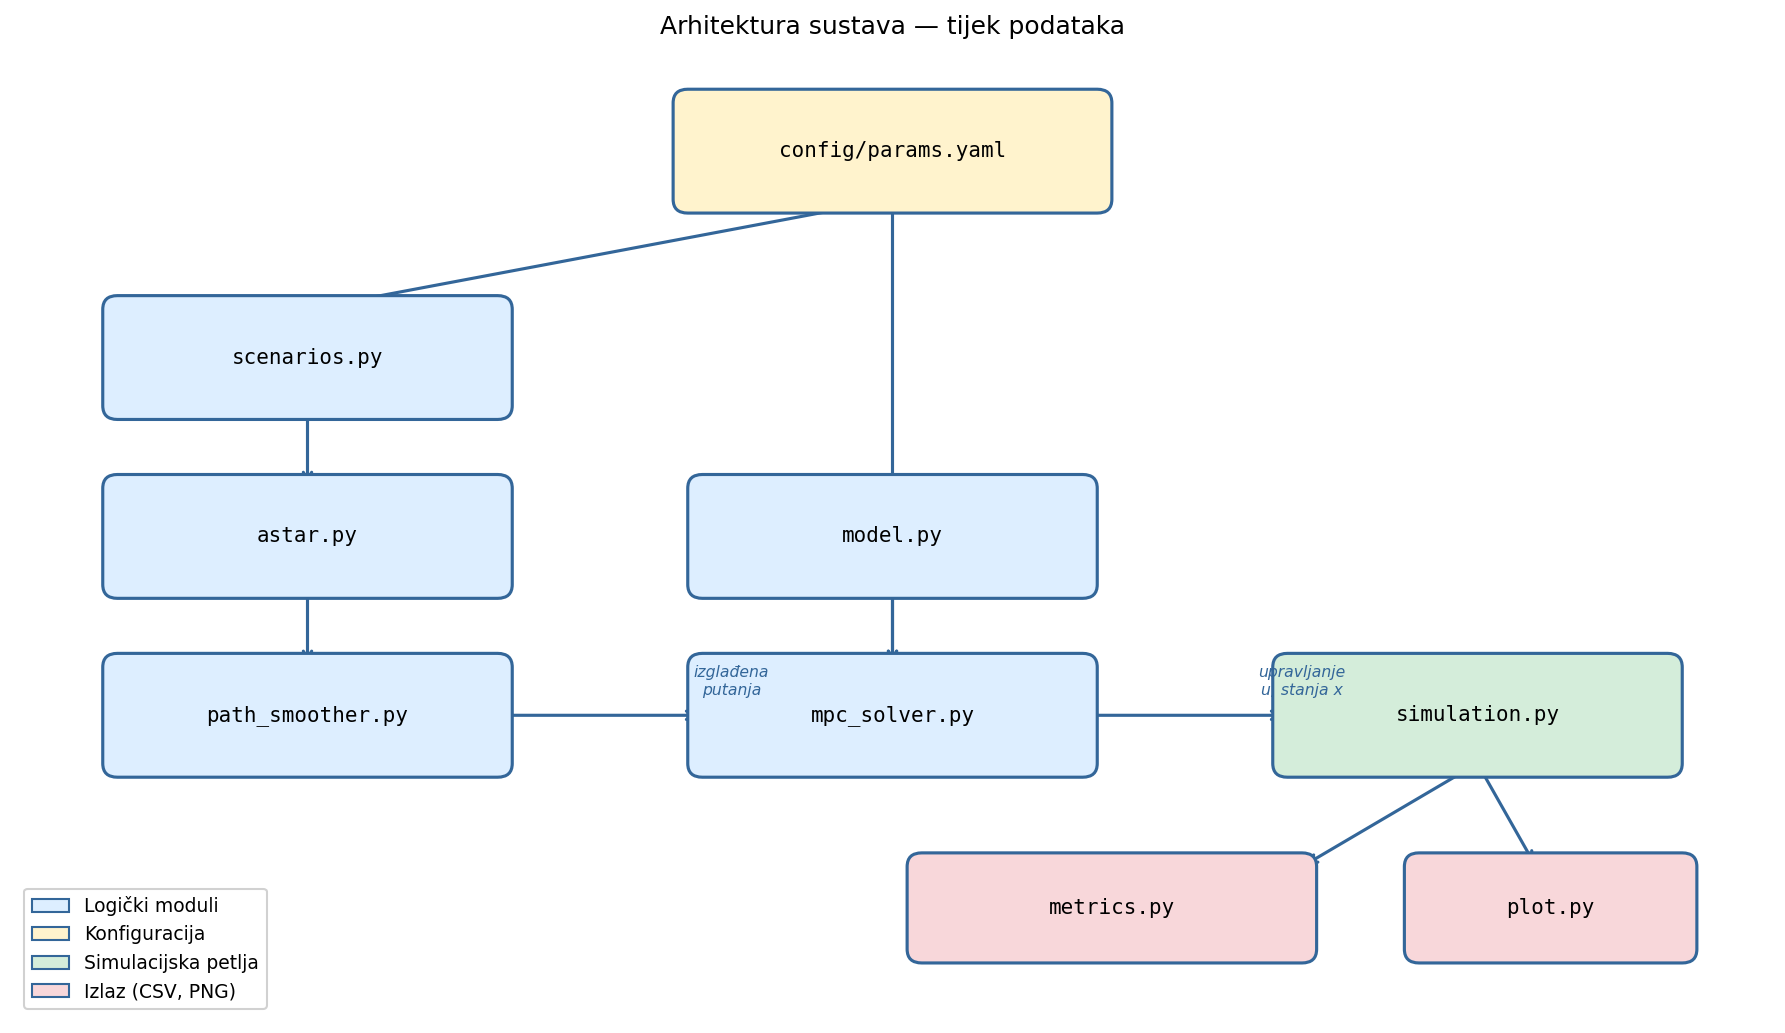
\includegraphics[width=0.95\linewidth]{figures/architecture.png}
  \caption{Arhitektura sustava. Konfiguracija (\texttt{params.yaml}) napaja sve module parametrima. Lijevi stupac prikazuje put planiranja putanje, sredina solver, a desno simulacijsku petlju i izlaz.}
  \label{slk:architecture}
\end{figure}

\section{Simulacijska petlja zatvorene petlje}
\label{sec:simloop}

Srž sustava je simulacijska petlja u \texttt{src/simulation.py}. Na svakom koraku:

\begin{enumerate}
  \item pronađe se najbliža sljedeća putna točka na putanji
  \item postavi se referenca $\mathbf{y}_{ref}$ za svih $N$ koraka horizonta
  \item fiksira se trenutno stanje kao početni uvjet OCP-a
  \item poziva se \texttt{solver.solve()} koji izvršava SQP\_RTI iteraciju
  \item uzima se prvi upravljački signal $\mathbf{u}_0^*$
  \item integrira se model RK4 metodom
  \item primjenjuje se eventualni poremećaj
\end{enumerate}

\begin{listing}[H]
\begin{minted}{python}
for step in range(max_steps):
    # napreduj do najbliže sljedeće putne točke
    while wp_idx < len(waypoints) - 1:
        if np.linalg.norm(x[:2] - waypoints[wp_idx+1]) \
                <= np.linalg.norm(x[:2] - waypoints[wp_idx]):
            wp_idx += 1
        else:
            break

    # postavi referencu za N koraka unaprijed
    for k in range(N):
        ref_idx = min(wp_idx + k, len(waypoints) - 1)
        xr, yr = waypoints[ref_idx]                    # koordinate ciljne putne točke
        dx = waypoints[min(ref_idx+1, len(waypoints)-1)][0] - xr
        dy = waypoints[min(ref_idx+1, len(waypoints)-1)][1] - yr
        theta_ref = np.arctan2(dy, dx)                 # smjer putanje u toj točki
        solver.set(k, "yref", np.array([xr, yr, theta_ref, 0.0, 0.0]))

    # fiksiraj trenutno stanje kao početni uvjet
    solver.set(0, "lbx", x)
    solver.set(0, "ubx", x)

    solver.solve()                    # jedna SQP_RTI iteracija
    u = solver.get(0, "u")           # uzmi prvi upravljački signal
    x = _rk4_step(x, u, dt)         # integriraj simulirani robot

    if np.linalg.norm(x[:2] - goal) < tol:
        break                         # cilj dosegnut
\end{minted}
\caption{Jezgra simulacijske petlje u \texttt{src/simulation.py}}
\end{listing}

\begin{figure}[H]
  \centering
  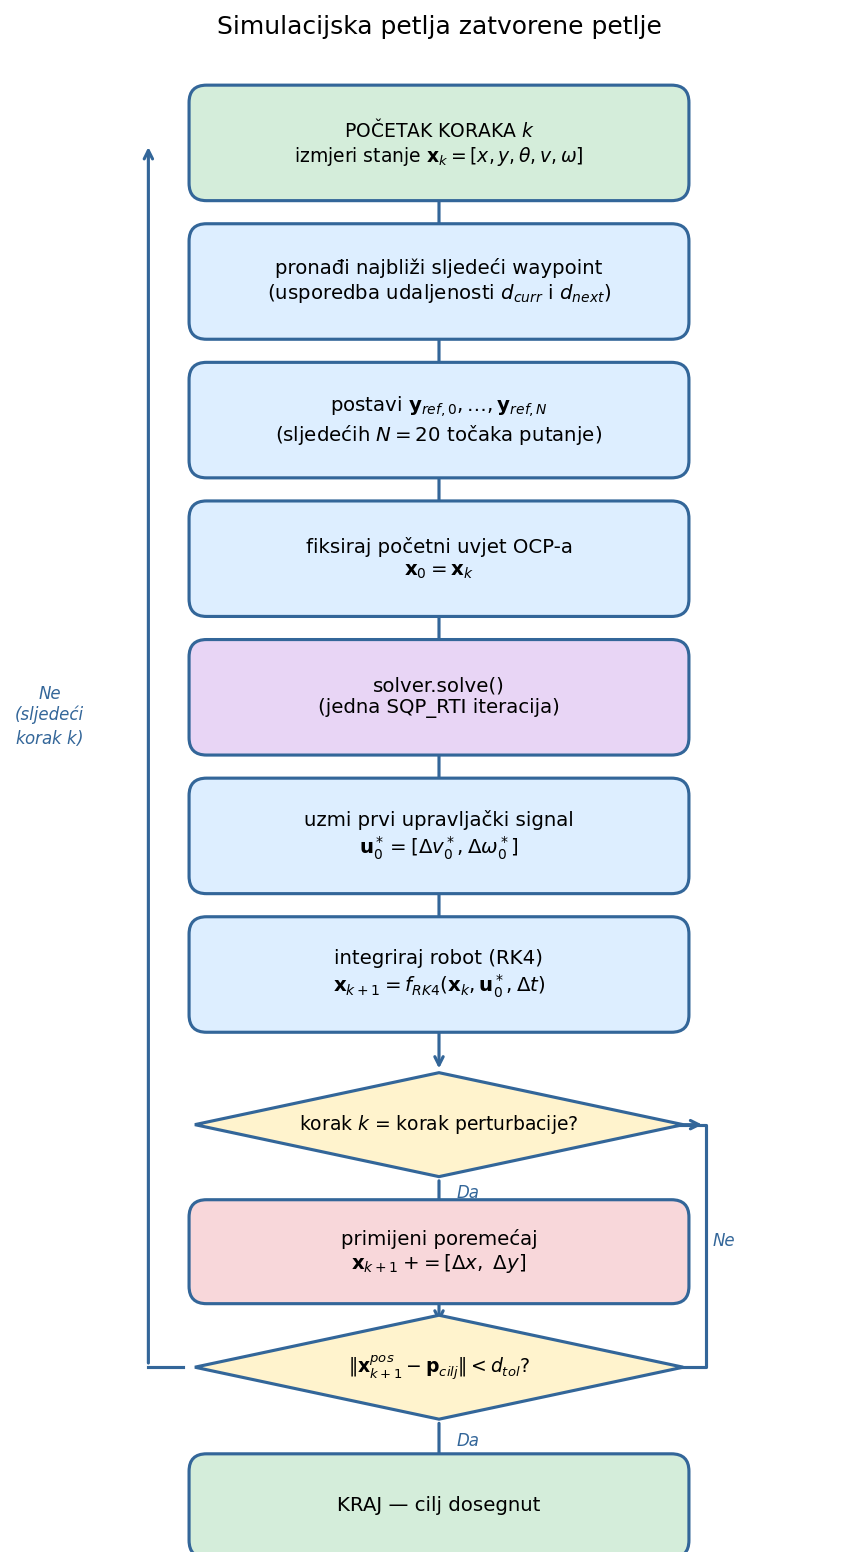
\includegraphics[width=0.52\linewidth]{figures/simulation_loop.png}
  \caption{Dijagram toka simulacijske petlje zatvorene petlje. Ljubičasti blok označava SQP\_RTI korak solvera, crveni blok primjenu poremećaja (prisutan samo u perturbacijskom scenariju).}
  \label{slk:simulation_loop}
\end{figure}

Napredak po putanji određuje se usporedbom udaljenosti. Na svakom koraku algoritam izračunava $d_{curr} = \|\mathbf{p} - \mathbf{w}_{idx}\|$ i $d_{next} = \|\mathbf{p} - \mathbf{w}_{idx+1}\|$ te pomiče indeks naprijed sve dok vrijedi $d_{next} \leq d_{curr}$. Uvjet se provjerava u petlji pa robot može preskočiti više putnih točaka odjednom pri većim brzinama. Slika~\ref{slk:waypoint_tracking} ilustrira mehanizam: dok je robot blizu $w_2$, vrijedi $d_{next} \gg d_{curr}$ i indeks stoji; čim robot prijeđe polovicu puta prema $w_3$, sljedeća putna točka postaje bliža i indeks se pomiče. Na taj način referentna točka uvijek odgovara stvarnoj poziciji robota u prostoru.

\begin{figure}[H]
  \centering
  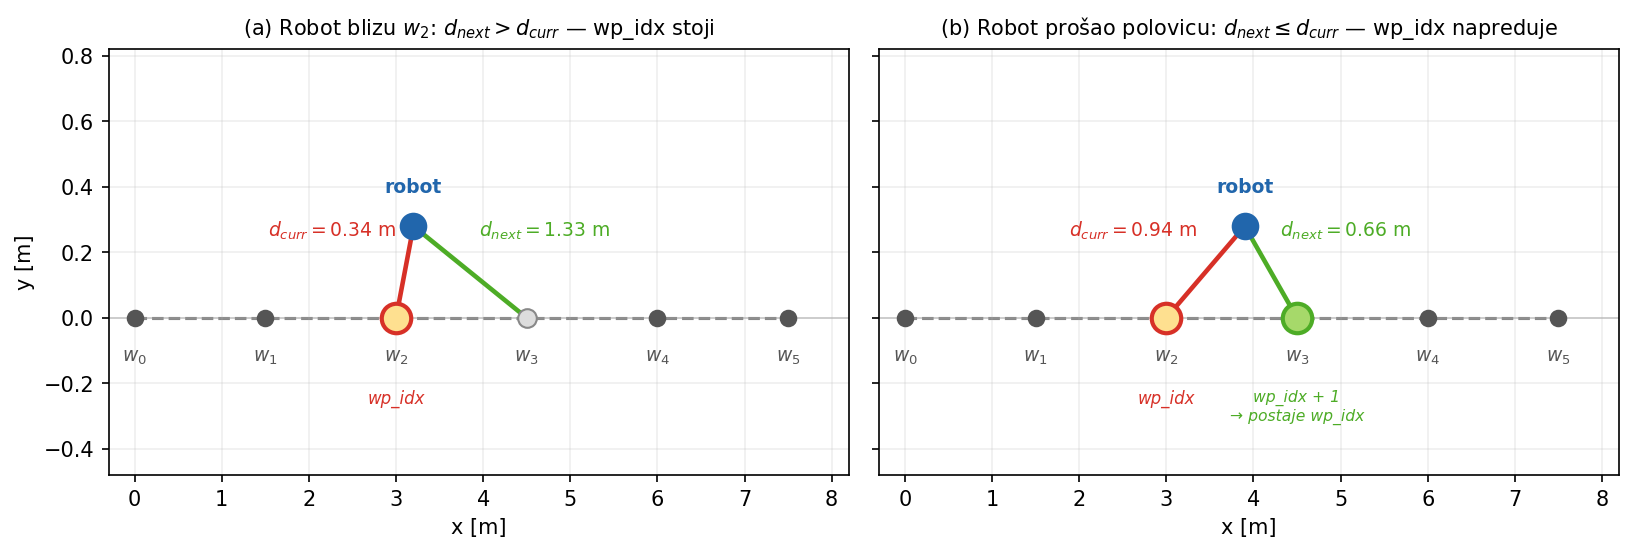
\includegraphics[width=0.95\linewidth]{figures/waypoint_tracking.png}
  \caption{Mehanizam napredovanja indeksa \texttt{wp\_idx}. Lijevo: robot je blizu $w_2$, vrijedi $d_{next} \gg d_{curr}$ i indeks stoji. Desno: robot je prešao polovicu segmenta prema $w_3$, vrijedi $d_{next} \leq d_{curr}$ i indeks napreduje.}
  \label{slk:waypoint_tracking}
\end{figure}

\section{Metrike kvalitete praćenja}

Modul \texttt{src/metrics.py} izračunava četiri mjere kvalitete iz rezultata simulacije.

\textbf{RMSE} (eng.\ \textit{Root Mean Square Error}) mjeri prosječno odstupanje od referentne putanje:

\begin{equation}
  \text{RMSE} = \sqrt{\frac{1}{K} \sum_{k=0}^{K-1} d_k^2}, \qquad d_k = \min_j \|\mathbf{p}_k - \mathbf{w}_j\|_2
\end{equation}

gdje je $d_k$ udaljenost od najbliže točke na putanji u koraku $k$. U implementaciji se za svaki vremenski korak izračunava udaljenost do svake točke izglađene putanje i uzima se minimum:

\begin{listing}[H]
\begin{minted}{python}
dists = np.linalg.norm(path - state[:2], axis=1)
idx   = np.argmin(dists)
d_k   = dists[idx]
\end{minted}
\caption{Izračun udaljenosti $d_k$ za RMSE u \texttt{src/metrics.py}}
\end{listing}

\textbf{CTE} (eng.\ \textit{Cross-Track Error}) mjeri okomitu udaljenost od segmenta putanje --- za razliku od RMSE-a uzima u obzir smjer putanje:

\begin{equation}
  \text{CTE}_k = \left| (\mathbf{p}_k - \mathbf{w}_{j^*}) \times \hat{\mathbf{t}}_{j^*} \right|
\end{equation}

gdje je $\hat{\mathbf{t}}_{j^*}$ smjer putanje u najbližoj točki $w_{j^*}$. Implementacija koristi skalarni oblik dvodimenzionalnog vektorskog produkta:

\begin{listing}[H]
\begin{minted}{python}
seg      = path[idx + 1] - path[idx]
seg_norm = seg / np.linalg.norm(seg)
diff     = state[:2] - path[idx]
cte      = abs(diff[0] * seg_norm[1] - diff[1] * seg_norm[0])
\end{minted}
\caption{Izračun CTE u \texttt{src/metrics.py}}
\end{listing}

\textbf{Greška smjera} (eng.\ \textit{heading error}) je apsolutna kutna razlika između orijentacije robota i smjera putanje, izračunata korištenjem atan2 za ispravno rukovanje kutnim prelaskom:

\begin{equation}
  e_{\theta,k} = \left| \text{atan2}(\sin(\theta_k - \theta_{ref,k}),\ \cos(\theta_k - \theta_{ref,k})) \right|
\end{equation}

Direktno oduzimanje kutova $\theta_k - \theta_{ref,k}$ nije ispravno jer rezultat može izaći iz intervala $(-\pi, \pi]$; formulacija s funkcijom \texttt{atan2} osigurava da greška uvijek ostaje unutar tog intervala.

\begin{listing}[H]
\begin{minted}{python}
theta_ref = np.arctan2(seg[1], seg[0])
he = abs(np.arctan2(np.sin(state[2] - theta_ref),
                     np.cos(state[2] - theta_ref)))
\end{minted}
\caption{Izračun greške smjera u \texttt{src/metrics.py}}
\end{listing}

Geometrijska interpretacija sve tri mjere prikazana je na slici~\ref{slk:metrics_concept}.

\begin{figure}[H]
  \centering
  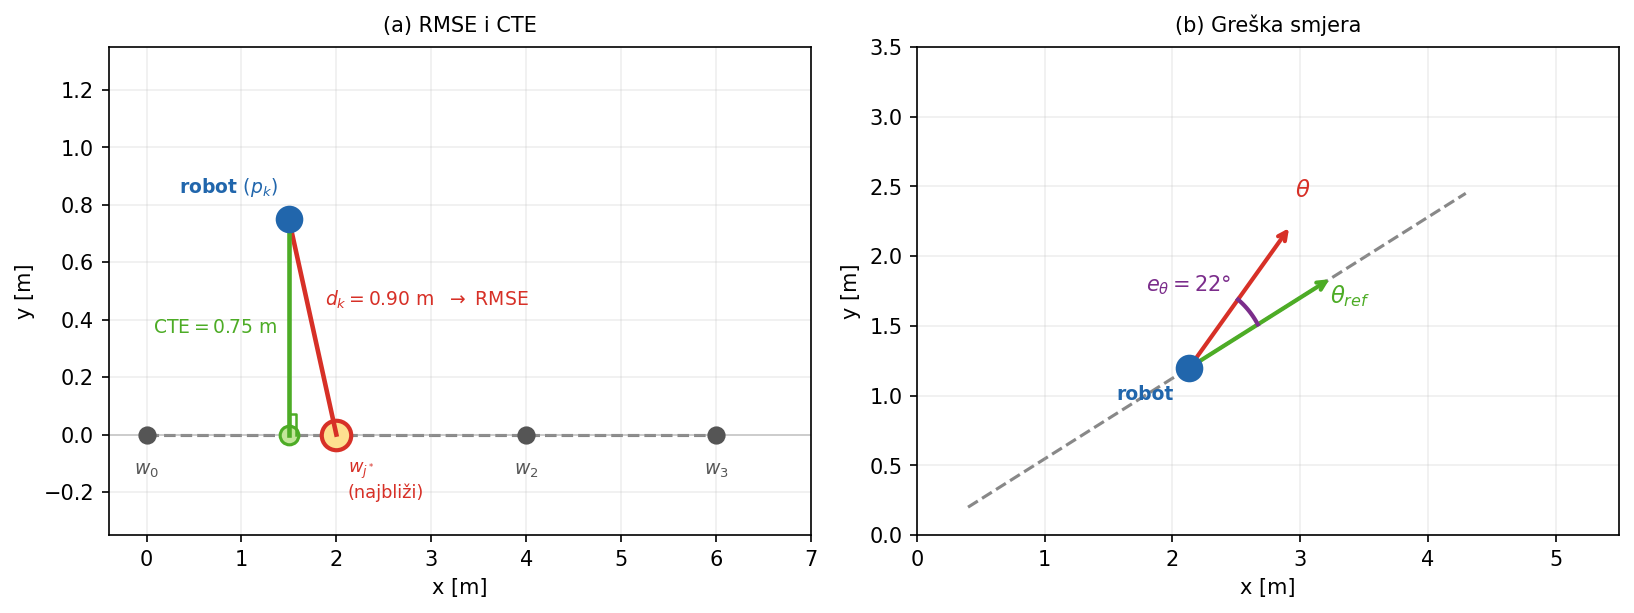
\includegraphics[width=0.95\linewidth]{figures/metrics_concept.png}
  \caption{Geometrijska interpretacija mjera kvalitete. Lijevo: RMSE mjeri udaljenost do najbliže putne točke $w_{j^*}$ (crvena linija $d_k$), dok CTE mjeri okomitu udaljenost do segmenta putanje (zelena linija). Desno: greška smjera $e_\theta$ je kutna razlika između orijentacije robota $\theta$ i referentnog smjera putanje $\theta_{ref}$.}
  \label{slk:metrics_concept}
\end{figure}

\textbf{CPU vrijeme} mjeri se funkcijom \texttt{time.perf\_counter()} neposredno oko svakog poziva \texttt{solver.solve()}, a bilježe se prosječno i maksimalno vrijeme po simulaciji:

\begin{listing}[H]
\begin{minted}{python}
t0 = time.perf_counter()
solver.solve()
solve_times.append(time.perf_counter() - t0)
\end{minted}
\caption{Mjerenje CPU vremena jedne SQP\_RTI iteracije u \texttt{src/simulation.py}}
\end{listing}

\section{Testni scenariji}

Sustav je testiran na osam scenarija različite složenosti: sedam u kojima robot uspješno dostiže cilj te jedan (\texttt{blocked}) koji testira prepoznavanje neizvedivog puta. U preostalim poglavljima pojam ``sedam scenarija'' odnosi se na ovih sedam navigacijskih scenarija, isključujući \texttt{blocked}. Tablica~\ref{tab:scenariji} prikazuje ključne karakteristike svih osam scenarija.

\begin{table}[H]
\centering
\caption{Pregled testnih scenarija}
\label{tab:scenariji}
\begin{tabular}{llll}
\toprule
Scenarij & Start & Cilj & Prepreke \\
\midrule
baseline     & $(0{,}5;\; 0{,}5)$ & $(9{,}5;\; 9{,}5)$ & — \\
one\_obstacle & $(0{,}5;\; 0{,}5)$ & $(9{,}5;\; 9{,}5)$ & 1 krug $r=1{,}0$ m \\
narrow       & $(0{,}5;\; 5{,}0)$ & $(9{,}5;\; 5{,}0)$ & 2 kruga $r=1{,}2$ m \\
l\_corridor  & $(0{,}5;\; 1{,}0)$ & $(9{,}0;\; 9{,}0)$ & 1 pravokutnik \\
u\_shape     & $(5{,}0;\; 0{,}5)$ & $(5{,}0;\; 9{,}5)$ & 3 pravokutnika \\
perturbation & $(0{,}5;\; 5{,}0)$ & $(9{,}5;\; 5{,}0)$ & — ($\Delta y = +1{,}0$ m u $t=3$ s) \\
cluttered    & $(0{,}5;\; 0{,}5)$ & $(9{,}5;\; 9{,}5)$ & 7 krugova \\
blocked      & $(0{,}5;\; 5{,}0)$ & $(9{,}5;\; 5{,}0)$ & 5 krugova (zid) \\
\bottomrule
\end{tabular}
\end{table}

Scenarij \texttt{blocked} je poseban --- A* ne može pronaći put pa se NMPC solver uopće ne pokreće. Sustav to prepoznaje i prikazuje kartu s porukom o neizvedivosti, što je opisano u poglavlju~\ref{pog:rezultati}.

Svaki scenarij definiran je kao Python rječnik koji vraća funkcija u \texttt{src/scenarios.py}. Primjer scenarija s uskim prolazom između dviju kružnih prepreka:

\begin{listing}[H]
\begin{minted}{python}
def _narrow():
    return {
        "name": "narrow",
        "start": np.array([0.5, 5.0, 0.0]),
        "goal":  np.array([9.5, 5.0]),
        "obstacles": [
            Circle(5.0, 3.5, 1.2),
            Circle(5.0, 6.5, 1.2),
        ],
        "perturbation": None,
    }
\end{minted}
\caption{Definicija scenarija uskog prolaza u \texttt{src/scenarios.py}. Prepreke su instance klase \texttt{Circle(cx, cy, r)}; svi scenariji bez poremećaja imaju \texttt{perturbation: None}.}
\end{listing}

% !TEX root = ../zavrsni_rad.tex

\chapter{Rezultati i evaluacija}
\label{pog:rezultati}

U ovom poglavlju prikazano je kako se sustav ponaša u praksi. Za svaki od sedam testnih scenarija prikazane su trajektorija robota, upravljački signali i greška praćenja, te su izmjereni pokazatelji kvalitete. Nakon toga analizirano je kako promjena dva ključna parametra sustava --- predikcijskog horizonta $N$ i težina troška --- utječe na preciznost i brzinu izvođenja. Poglavlje završava tablicom usporedbe svih scenarija.

\FloatBarrier
% ─────────────────────────────────────────────────────────────────────────────
\section{Eksperimentalni postav}
\label{sec:r_postav}

Sva ispitivanja provedena su u simulacijskom okruženju implementiranom u Pythonu, korištenjem acados solvera za rješavanje OCP-a. Simulacijsko okruženje modelira ravnu površinu dimenzija $10\ \text{m} \times 10\ \text{m}$. Simulacija se odvija u zatvorenoj petlji s korakom uzorkovanja $\Delta t = 0{,}1$ s i završava kada robot dođe unutar $d_{tol} = 0{,}3$ m od cilja ili po isteku $k_{max} = 1000$ koraka. Metrike evaluacije definirane su u poglavlju~\ref{pog:implementacija}, a pregled testnih scenarija u tablici~\ref{tab:scenariji}.

Sva mjerenja izvršena su na prijenosnom računalu s procesorom Intel Core 7 150U i 32 GB RAM-a, pod operacijskim sustavom Fedora 42 (Linux kernel 6.19.14). Korišteni softver: Python 3.13.13, acados 0.5.1, CasADi 3.7.2, SciPy 1.17.1; solver je kompajliran kompajlerom GCC 15.2.1. CPU vrijeme jednog koraka mjereno je funkcijom \texttt{time.perf\_counter()} neposredno oko poziva \texttt{solver.solve()} (prikazano u listingu u poglavlju~\ref{pog:implementacija}).

Tablica~\ref{tab:params} prikazuje sve ključne parametre korištene u eksperimentima.

\begin{table}[H]
\centering
\caption{Parametri simulacijskog okruženja}
\label{tab:params}
\begin{tabular}{llll}
\toprule
Skupina & Parametar & Oznaka & Vrijednost \\
\midrule
\textbf{Robot} & Polumjer & $r_{rob}$ & $0{,}2$ m \\
 & Maksimalna brzina & $v_{max}$ & $1{,}0$ m/s \\
 & Minimalna brzina & $v_{min}$ & $0{,}05$ m/s \\
 & Maksimalna kutna brzina & $\omega_{max}$ & $1{,}5$ rad/s \\
 & Maks.\ translacijsko ubrzanje & $a_{v,max}$ & $0{,}5$ m/s\textsuperscript{2} \\
 & Maks.\ kutno ubrzanje & $\alpha_{max}$ & $1{,}0$ rad/s\textsuperscript{2} \\
\midrule
\textbf{NMPC} & Predikcijski horizont & $N$ & 20 koraka \\
 & Korak uzorkovanja & $\Delta t$ & $0{,}1$ s \\
 & Težine pozicije & $Q_x, Q_y$ & $10{,}0$ \\
 & Težina orijentacije & $Q_\theta$ & $1{,}0$ \\
 & Terminalna težinska matrica & $W_e$ & $Q$ \\
 & Težine upravljanja & $R_{a_v}, R_{\alpha}$ & $0{,}1$ \\
 & Vrsta ograničenja prepreka & — & meka (soft) \\
 & Vrsta solvera & — & SQP\_RTI \\
\midrule
\textbf{A*} & Rezolucija mreže & $d_{grid}$ & $0{,}2$ m \\
 & Ukupna inflacija prepreka & $d_{inf}$ & $0{,}4$ m ($0{,}2$ sigurnost $+$ $0{,}2$ polumjer) \\
\midrule
\textbf{Simulacija} & Tolerancija cilja & $d_{tol}$ & $0{,}3$ m \\
 & Integrator & — & RK4 \\
 & Maks.\ broj koraka & $k_{max}$ & $1000$ \\
\bottomrule
\end{tabular}
\end{table}

Konfiguracija je pohranjena u datoteci \texttt{config/params.yaml}:

\begin{listing}[H]
\begin{minted}{yaml}
robot:
  radius: 0.2
  v_max: 1.0
  v_min: 0.05
  omega_max: 1.5
  dv_max: 0.5
  domega_max: 1.0
mpc:
  N: 20
  dt: 0.1
  Q: [10.0, 10.0, 1.0]
  R: [0.1, 0.1]
  solver_type: SQP_RTI
  constraints: soft
simulation:
  goal_tolerance: 0.3
  max_steps: 1000
\end{minted}
\caption{Ključni parametri u \texttt{config/params.yaml}}
\end{listing}

\FloatBarrier
% ─────────────────────────────────────────────────────────────────────────────
\section{Osnovna putanja}
\label{sec:r_baseline}

Scenarij osnovne putanje definira kretanje od $(0{,}5;\; 0{,}5)$ s orijentacijom $\theta_0 = 0$ do cilja $(9{,}5;\; 9{,}5)$, bez prepreka. Svrha je provjera ispravnosti sustava u idealnim uvjetima i uspostava referentnih vrijednosti za usporedbu s kompleksnijim scenarijima. A* planira dijagonalnu putanju koju algoritam glađenja pretvara u glatku krivulju duljine oko 12,7 m.

\begin{figure}[htbp]
  \centering
  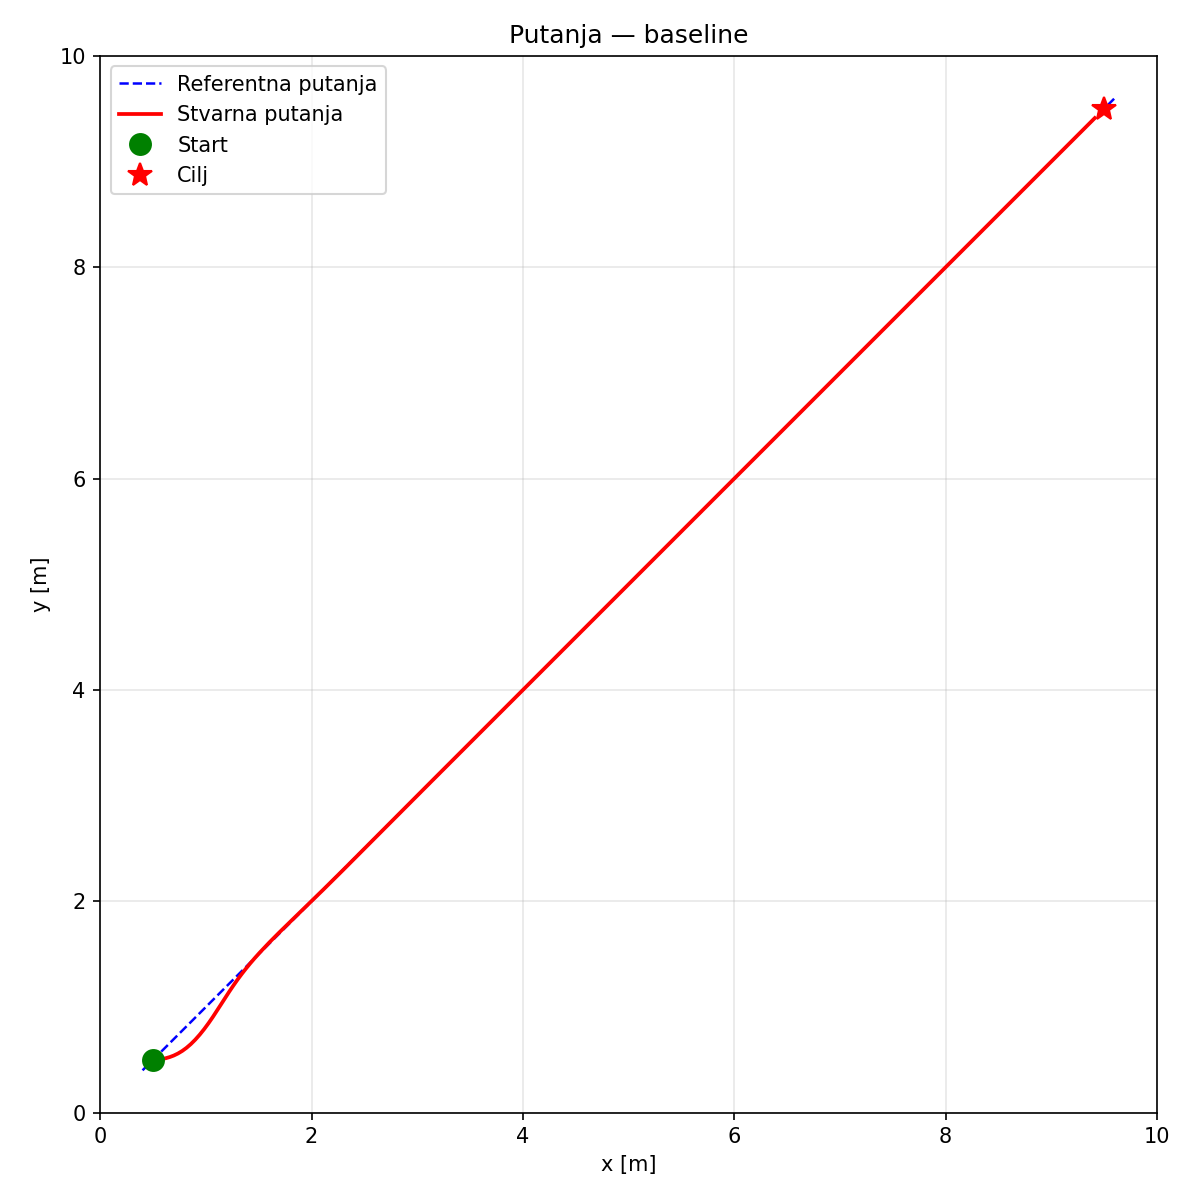
\includegraphics[width=0.82\linewidth]{figures/baseline_traj.png}
  \caption{Referentna i stvarna putanja robota u scenariju bez prepreka.}
  \label{slk:baseline_traj}
\end{figure}

Slika~\ref{slk:baseline_traj} pokazuje da stvarna putanja prati referentnu s RMSE od $34{,}4$ mm. Jedino vidljivo odstupanje pojavljuje se na početku kretanja gdje robot s $\theta_0 = 0$ mora korigirati smjer prema dijagonalnom referentnom pravcu (kut $\approx 45°$). NMPC regulator ispravno prepoznaje taj zahtjev i robota glatko preusmjerava bez oscilacija.

\begin{figure}[htbp]
  \centering
  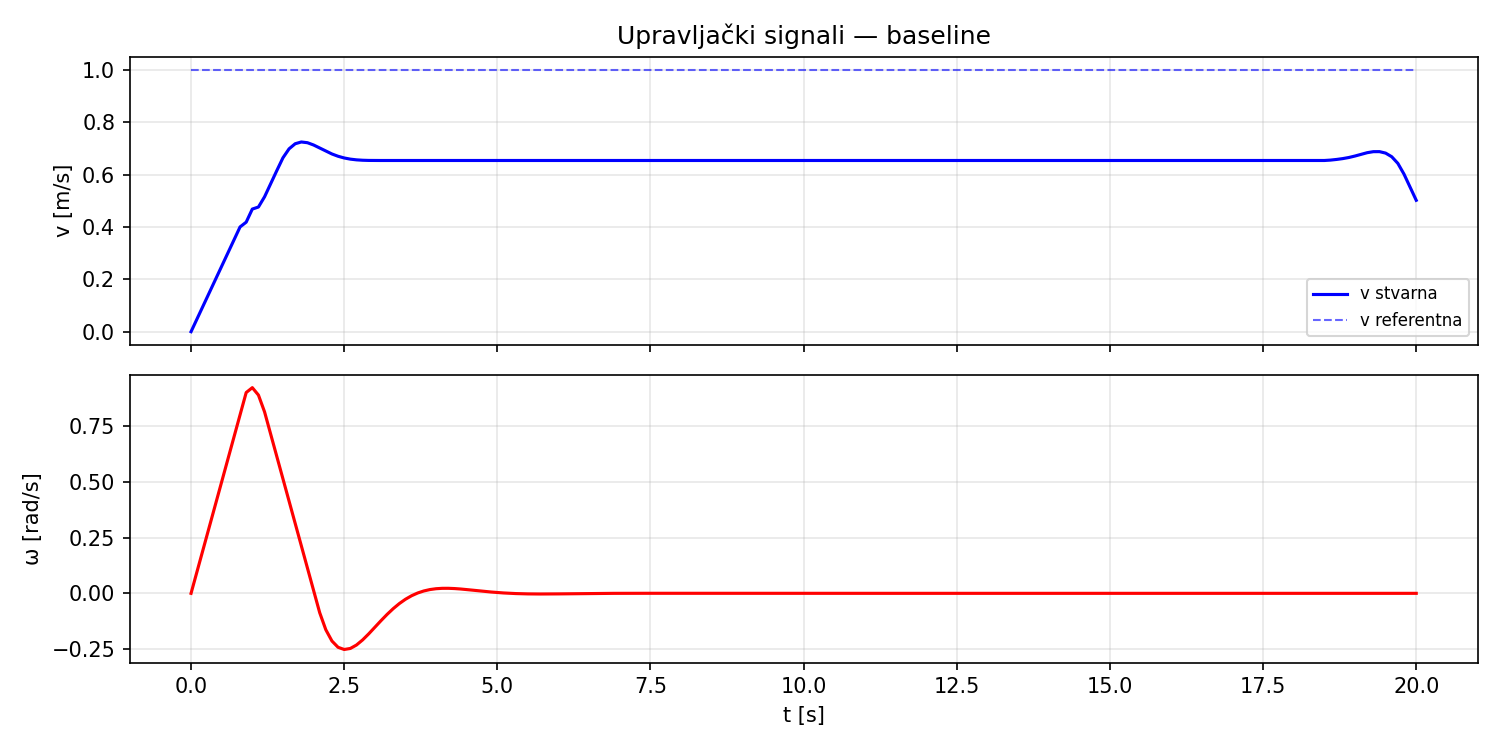
\includegraphics[width=0.82\linewidth]{figures/baseline_controls.png}
  \caption{Brzina $v(t)$ i kutna brzina $\omega(t)$ u scenariju bez prepreka.}
  \label{slk:baseline_controls}
\end{figure}

Graf upravljačkih signala (slika~\ref{slk:baseline_controls}) potvrđuje ispravno ponašanje: brzina $v$ raste do $v_{max} = 1{,}0$ m/s i ostaje na toj razini do blizine cilja, dok kutna brzina $\omega$ pokazuje vrh od $\approx 0{,}87$ rad/s u prvoj sekundi (inicijalna korekcija smjera), a potom se stabilizira blizu nule.

\begin{figure}[htbp]
  \centering
  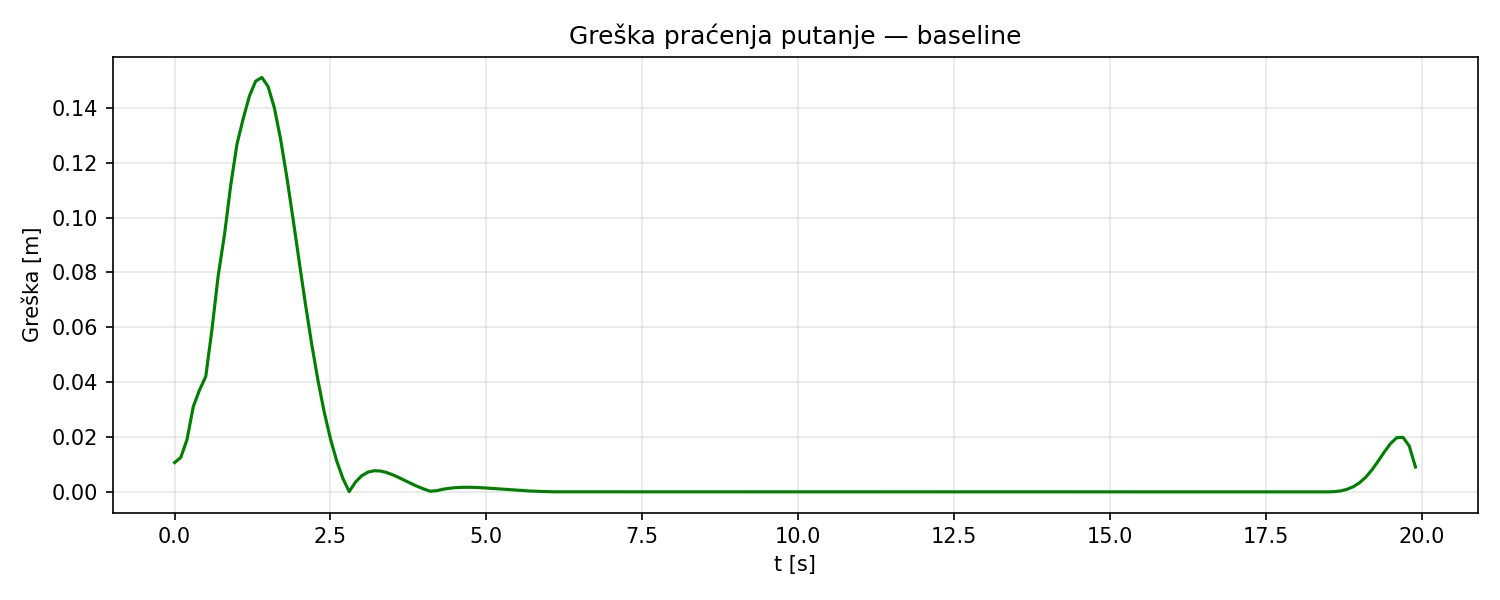
\includegraphics[width=0.82\linewidth]{figures/baseline_error.png}
  \caption{Greška praćenja u funkciji vremena za scenarij bez prepreka.}
  \label{slk:baseline_error}
\end{figure}

Graf greške (slika~\ref{slk:baseline_error}) prikazuje maksimum od $\approx 0{,}15$ m oko $t \approx 1{,}5$ s, što odgovara inicijalnoj korekciji smjera, a potom brzo opada ispod $0{,}03$ m.

\begin{table}[H]
\centering
\caption{Metrike --- osnovna putanja}
\label{tab:baseline}
\begin{tabular}{ll}
\toprule
Metrika & Vrijednost \\
\midrule
RMSE & $0{,}0344$ m \\
CTE srednji & $0{,}0107$ m \\
CTE max & $0{,}1478$ m \\
Greška smjera (srednja) & $2{,}73°$ \\
Vrijeme do cilja & $20{,}00$ s \\
CPU (prosjek / max) & $0{,}091$ ms / $0{,}319$ ms \\
Dostigao cilj & Da \\
\bottomrule
\end{tabular}
\end{table}

RMSE od $34{,}4$ mm i srednja bočna greška od $10{,}7$ mm potvrđuju visoku kvalitetu praćenja. Prosječno CPU vrijeme od $0{,}091$ ms po koraku iznosi manje od $0{,}1$\% trajanja uzornog intervala od $100$ ms, što pokazuje da je sustav primjenjiv u stvarnim uvjetima gdje je vrijeme odziva ključno.

\FloatBarrier
% ─────────────────────────────────────────────────────────────────────────────
\section{Jedna prepreka}
\label{sec:r_one_obstacle}

Scenarij uvodi kružnu prepreku polumjera $r = 1{,}0$ m u središte prostora u točki $(5{,}0;\; 5{,}0)$. Robot kreće iz $(0{,}5;\; 0{,}5)$ prema cilju $(9{,}5;\; 9{,}5)$, pa prepreka direktno blokira najkraću dijagonalnu putanju. A* pronalazi put koji zaobilazi prepreku s gornje lijeve strane.

\begin{figure}[htbp]
  \centering
  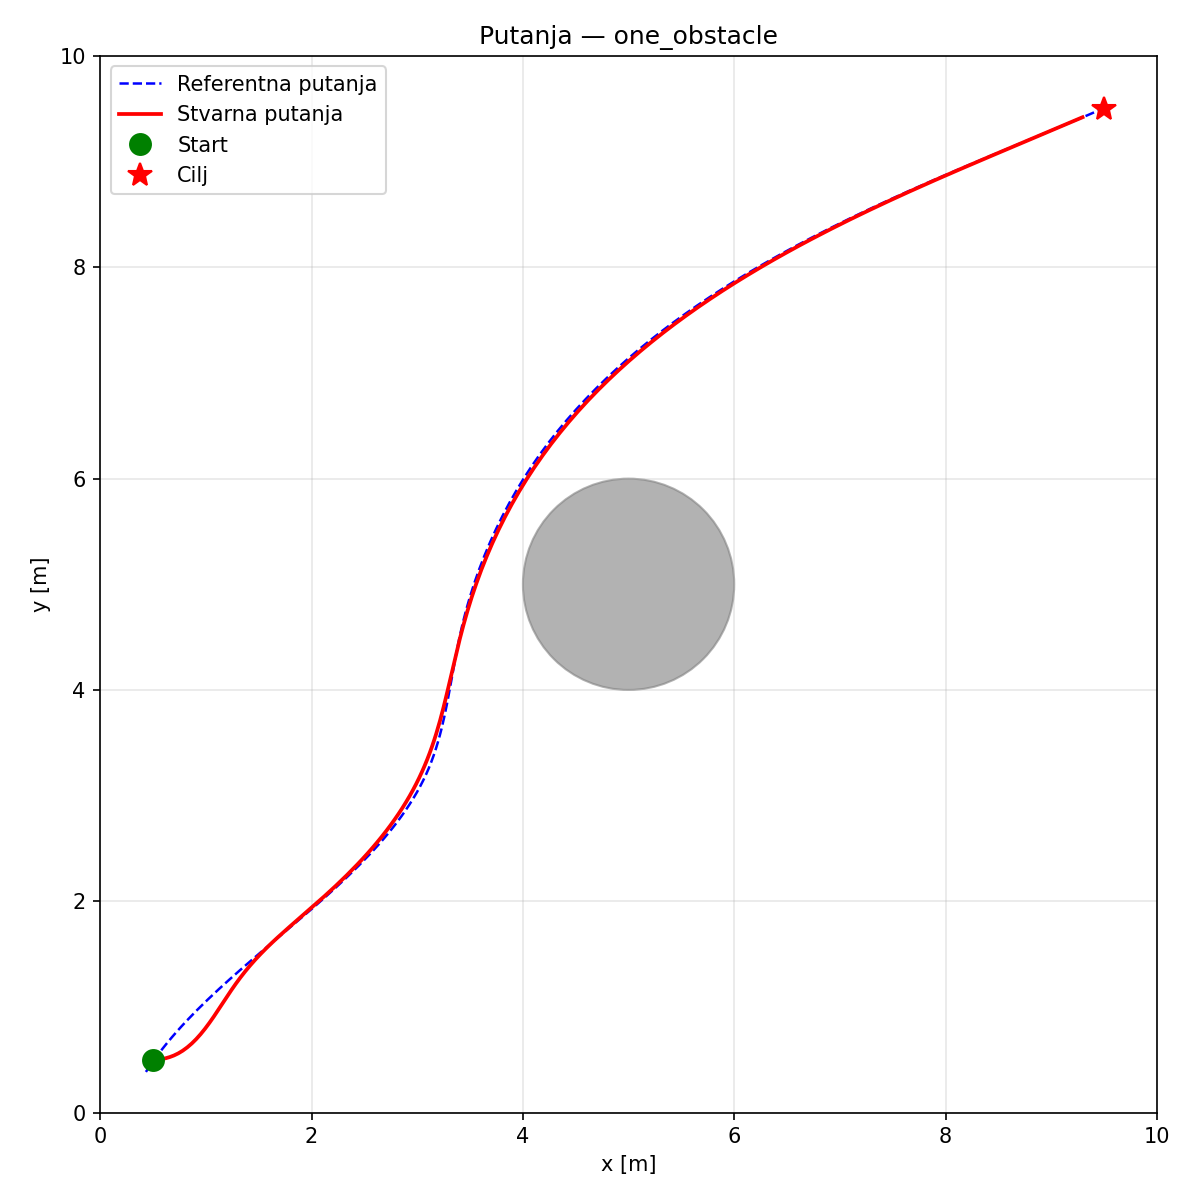
\includegraphics[width=0.82\linewidth]{figures/one_obstacle_traj.png}
  \caption{Referentna i stvarna putanja u scenariju s jednom kružnom preprekom. Robot zaobilazi prepreku s gornje lijeve strane.}
  \label{slk:one_obstacle_traj}
\end{figure}

Slika~\ref{slk:one_obstacle_traj} pokazuje da robot prati referentnu putanju s visokom točnošću, uključujući zavoj oko prepreke. Minimalna udaljenost od ruba prepreke iznosi više od $0{,}4$ m, što je iznad zbroja polumjera robota i sigurnosne margine, pa meka ograničenja prepreka u NMPC-u nisu bila aktivna.

\begin{figure}[htbp]
  \centering
  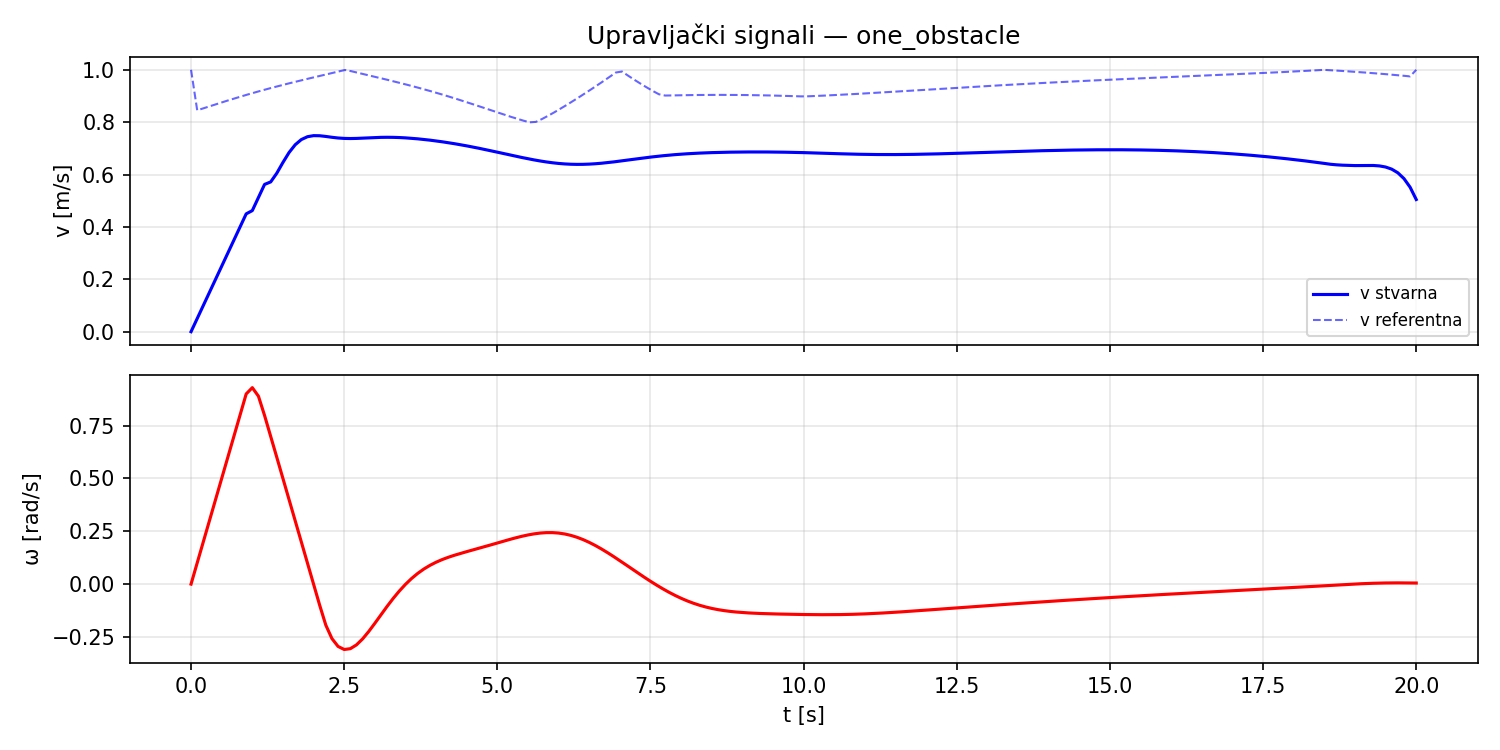
\includegraphics[width=0.82\linewidth]{figures/one_obstacle_controls.png}
  \caption{Brzina $v(t)$ i kutna brzina $\omega(t)$ u scenariju s jednom preprekom. Dva karakteristična vrha $\omega$ odgovaraju inicijalnoj korekciji smjera i zavoju oko prepreke.}
  \label{slk:one_obstacle_controls}
\end{figure}

\begin{figure}[htbp]
  \centering
  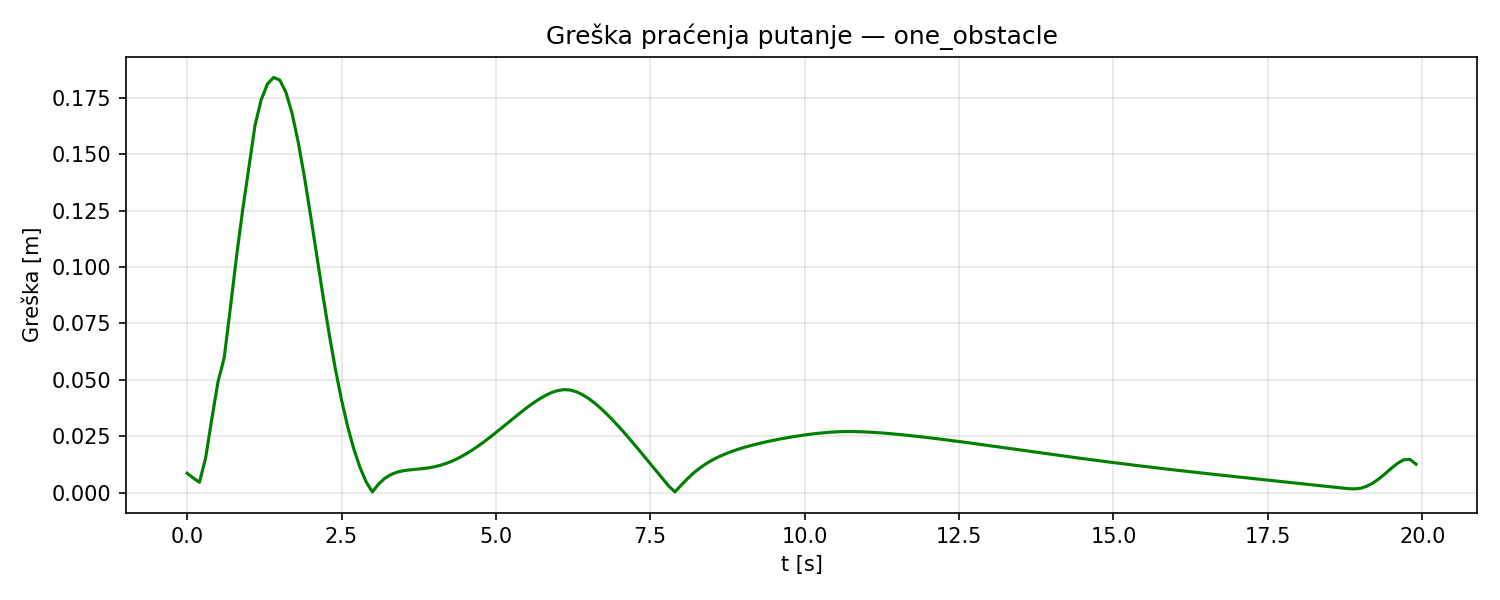
\includegraphics[width=0.82\linewidth]{figures/one_obstacle_error.png}
  \caption{Greška praćenja u scenariju s jednom preprekom.}
  \label{slk:one_obstacle_error}
\end{figure}

\begin{table}[H]
\centering
\caption{Metrike --- jedna prepreka}
\label{tab:one_obstacle}
\begin{tabular}{lll}
\toprule
Metrika & Vrijednost & Usporedba s osnovnim \\
\midrule
RMSE & $0{,}0469$ m & $+36{,}1$\% \\
CTE srednji & $0{,}0278$ m & $+160{,}7$\% \\
CTE max & $0{,}1839$ m & $+24{,}4$\% \\
Greška smjera (srednja) & $3{,}87°$ & $+42{,}0$\% \\
Vrijeme do cilja & $20{,}00$ s & $0$\% \\
CPU (prosjek / max) & $0{,}099$ ms / $0{,}359$ ms & $+8{,}8$\% \\
Dostigao cilj & Da & --- \\
\bottomrule
\end{tabular}
\end{table}

RMSE i CTE su veći nego u osnovnom scenariju jer putanja sada ima zavoj oko prepreke --- robot ne može trenutačno promijeniti smjer pa u krivini blago zaostaje za referencom. Unatoč tome, RMSE ostaje ispod $50$ mm, a dodatno CPU opterećenje ($+8{,}8$\%) je zanemarivo.

\FloatBarrier
% ─────────────────────────────────────────────────────────────────────────────
\section{Uski prolaz}
\label{sec:r_narrow}

Scenarij postavlja dvije kružne prepreke polumjera $r = 1{,}2$ m u točkama $(5{,}0;\; 3{,}5)$ i $(5{,}0;\; 6{,}5)$. Robot kreće iz $(0{,}5;\; 5{,}0)$ prema $(9{,}5;\; 5{,}0)$, pa referentna putanja prolazi upravo između tih prepreka.

Geometrijska analiza otkriva ključnu karakteristiku scenarija: uzimajući u obzir ukupnu inflaciju od $d_{inf} = 0{,}4$ m (sigurnosna margina $0{,}2$ m $+$ polumjer robota $0{,}2$ m), efektivna širina prolaza između infliranih prepreka iznosi:
\begin{equation}
  d_{prolaz} = (6{,}5 - 1{,}2 - 0{,}4) - (3{,}5 + 1{,}2 + 0{,}4) = 4{,}9 - 5{,}1 = -0{,}2 \text{ m}
\end{equation}

Negativna vrijednost znači da prolaz između prepreka nije prohodan za robota. A* zato planira put koji zaobilazi donju prepreku ispod nje, spuštajući putanju do $y \approx 2{,}2$ m.

\begin{figure}[htbp]
  \centering
  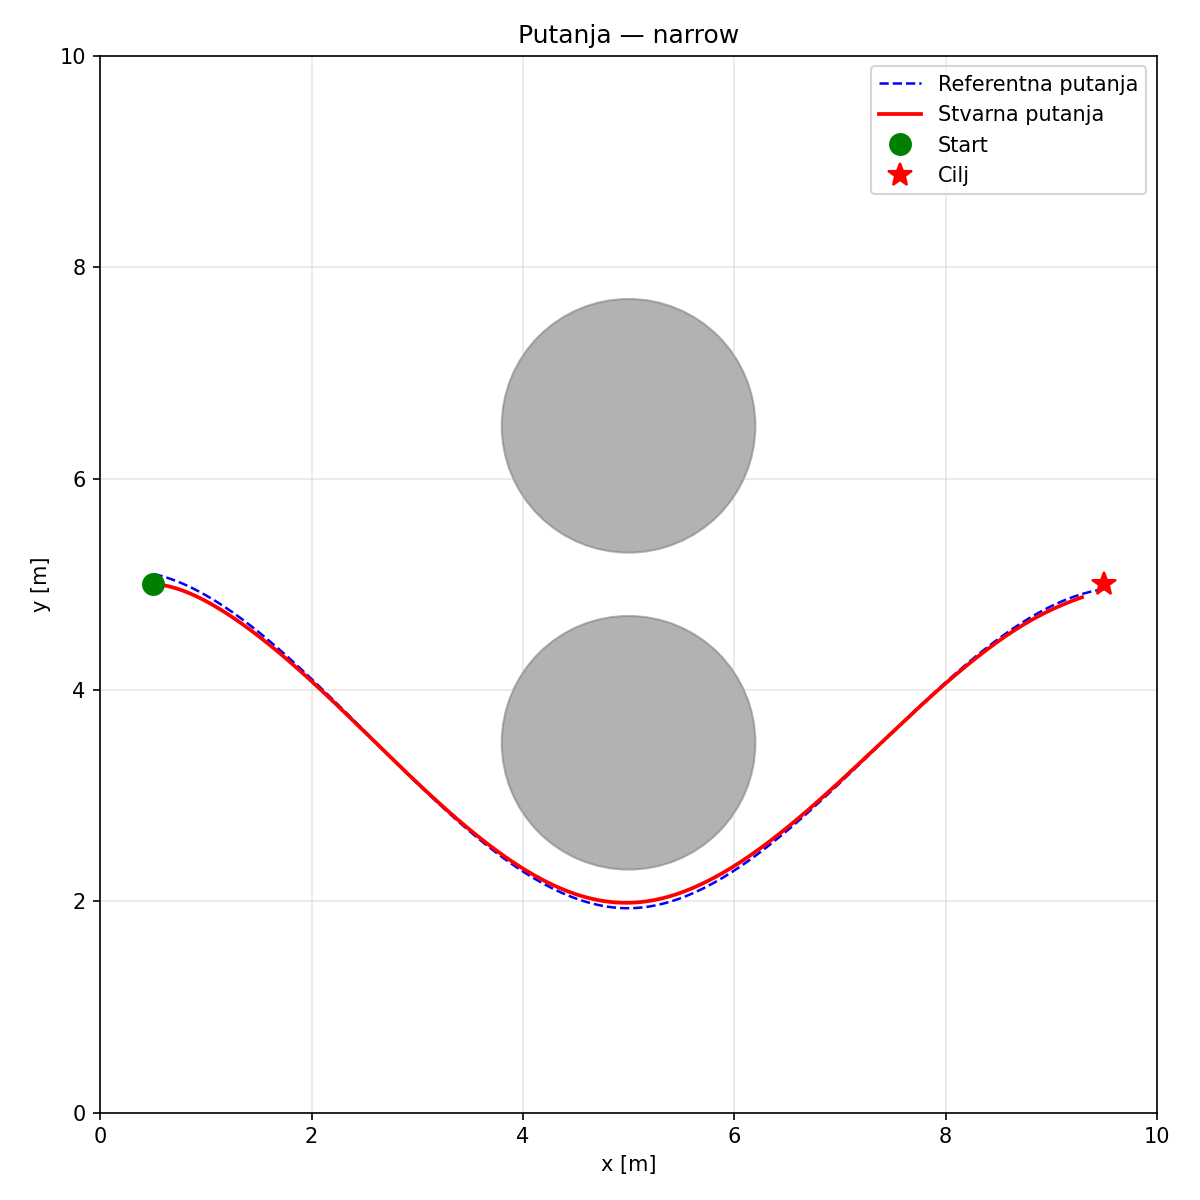
\includegraphics[width=0.82\linewidth]{figures/narrow_traj.png}
  \caption{Referentna i stvarna putanja u scenariju uskog prolaza. A* planira put ispod donje prepreke jer je prolaz između njih blokiran proširenim područjem prepreka.}
  \label{slk:narrow_traj}
\end{figure}

Slika~\ref{slk:narrow_traj} prikazuje karakteristični luk: robot se spušta prema jugu, prolazi ispod donje prepreke pri $y \approx 2{,}2$ m, a zatim se vraća prema ciljnoj koordinati $y = 5{,}0$ m. Robot prati zadanu putanju s visokom točnošću, a minimalna udaljenost od ruba donje prepreke iznosi oko $0{,}5$ m.

\begin{figure}[htbp]
  \centering
  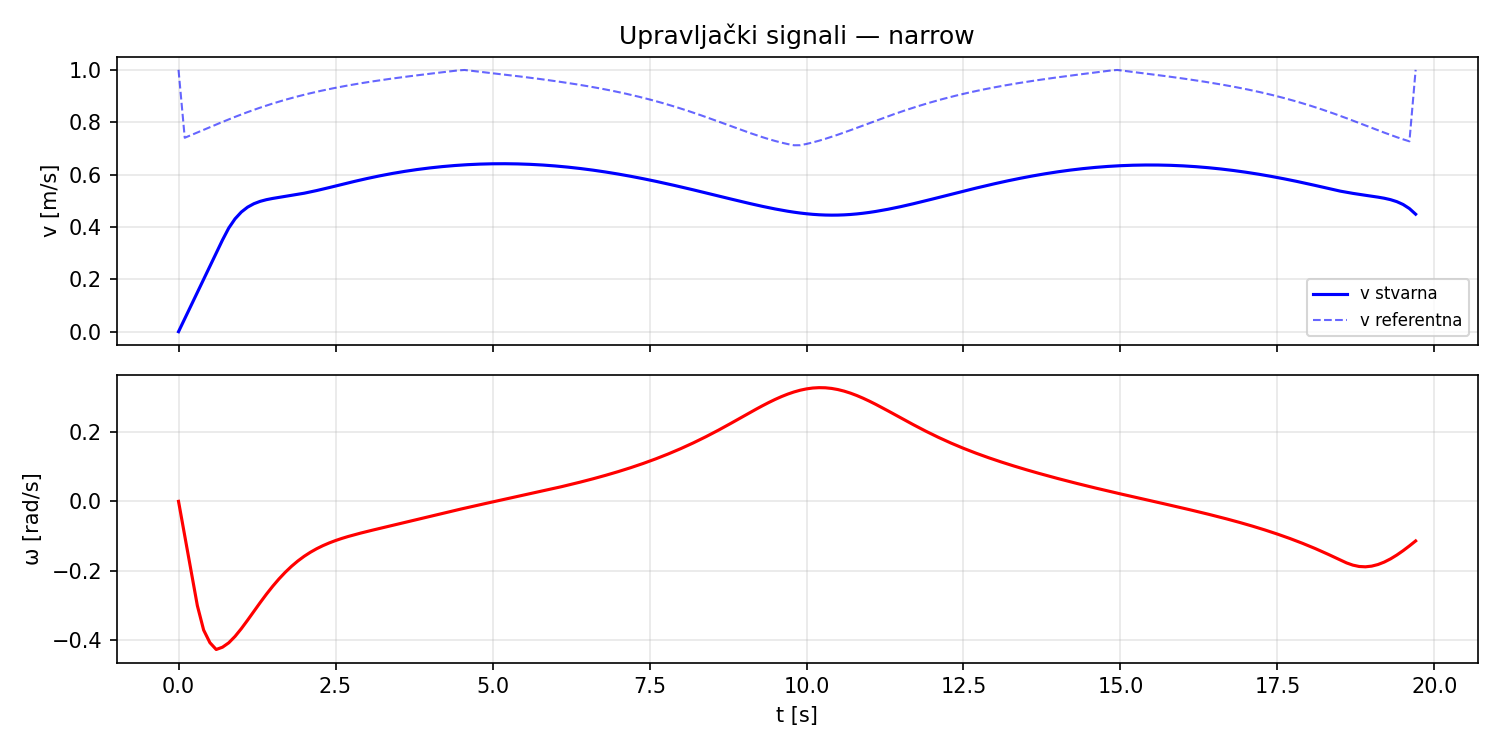
\includegraphics[width=0.82\linewidth]{figures/narrow_controls.png}
  \caption{Brzina $v(t)$ i kutna brzina $\omega(t)$ u scenariju uskog prolaza. Kontinuirani sinusoidalni profil $\omega$ odgovara zaobilaženju prepreke.}
  \label{slk:narrow_controls}
\end{figure}

\begin{figure}[htbp]
  \centering
  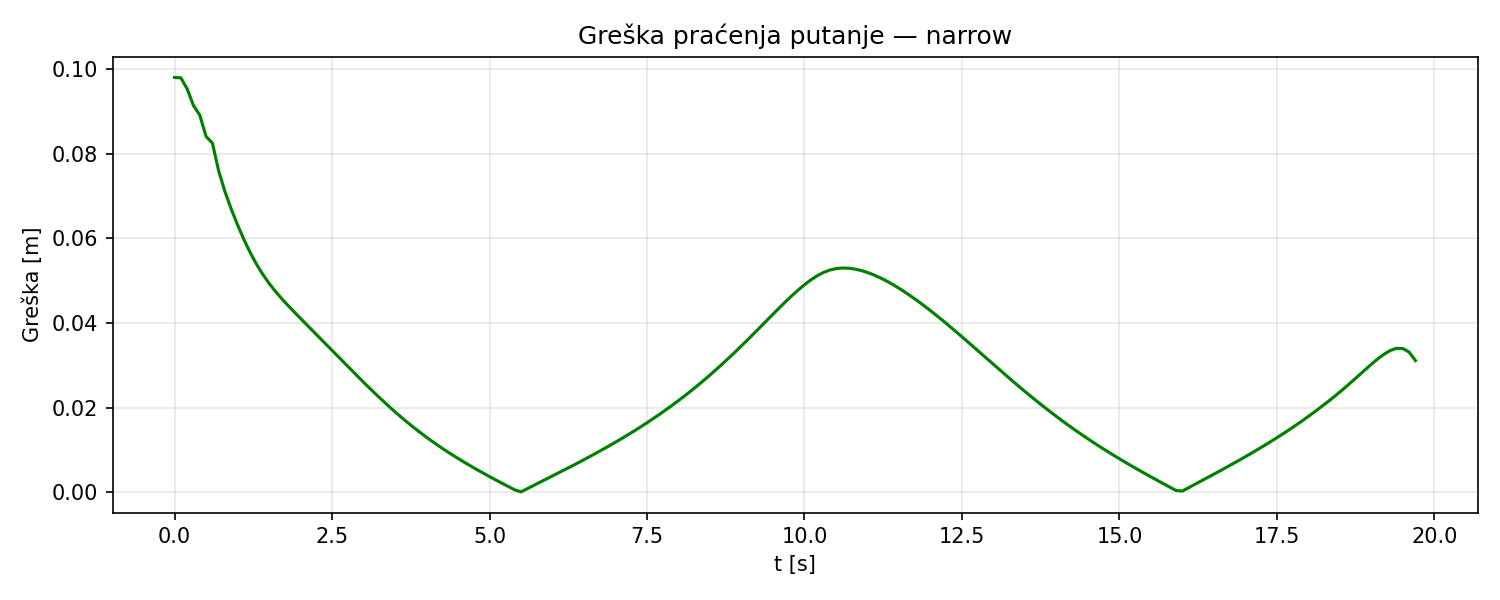
\includegraphics[width=0.82\linewidth]{figures/narrow_error.png}
  \caption{Greška praćenja u scenariju uskog prolaza. Dva područja povišene greške odgovaraju dvjema najizraženijim krivinama putanje.}
  \label{slk:narrow_error}
\end{figure}

\begin{table}[H]
\centering
\caption{Metrike --- uski prolaz}
\label{tab:narrow}
\begin{tabular}{lll}
\toprule
Metrika & Vrijednost & Usporedba s osnovnim \\
\midrule
RMSE & $0{,}0344$ m & $\approx 0$\% \\
CTE srednji & $0{,}0270$ m & $+152{,}7$\% \\
CTE max & $0{,}0962$ m & $-34{,}9$\% \\
Greška smjera (srednja) & $1{,}59°$ & $-41{,}5$\% \\
Vrijeme do cilja & $19{,}70$ s & $-1{,}5$\% \\
CPU (prosjek / max) & $0{,}089$ ms / $0{,}263$ ms & $-2{,}2$\% \\
Dostigao cilj & Da & --- \\
\bottomrule
\end{tabular}
\end{table}

Ostvareni RMSE ($34{,}4$ mm) jednak je onom iz osnovnog scenarija, a greška smjera ($1{,}59°$) je najmanji od svih scenarija. Razlog je jednostavan: robot kreće s početnom orijentacijom $\theta_0 = 0$ (prema desno) i cilj se nalazi upravo u tom smjeru, pa ne treba inicijalna korekcija kuta --- za razliku od osnovnog scenarija gdje je robot morao odmah skrenuti za $\approx 45°$.

\FloatBarrier
% ─────────────────────────────────────────────────────────────────────────────
\section{L-hodnik}
\label{sec:r_lcorridor}

U ovom scenariju velik pravokutni zid dimenzija $7{,}5\ \text{m} \times 6{,}5\ \text{m}$ blokira gornji lijevi dio prostora. Robot mora prijeći karakteristični L-oblik putanje: horizontalni prolaz duž donjeg ruba prepreke, a potom okret za $90°$ i vertikalni uspon uz njezin desni rub.

\begin{figure}[htbp]
  \centering
  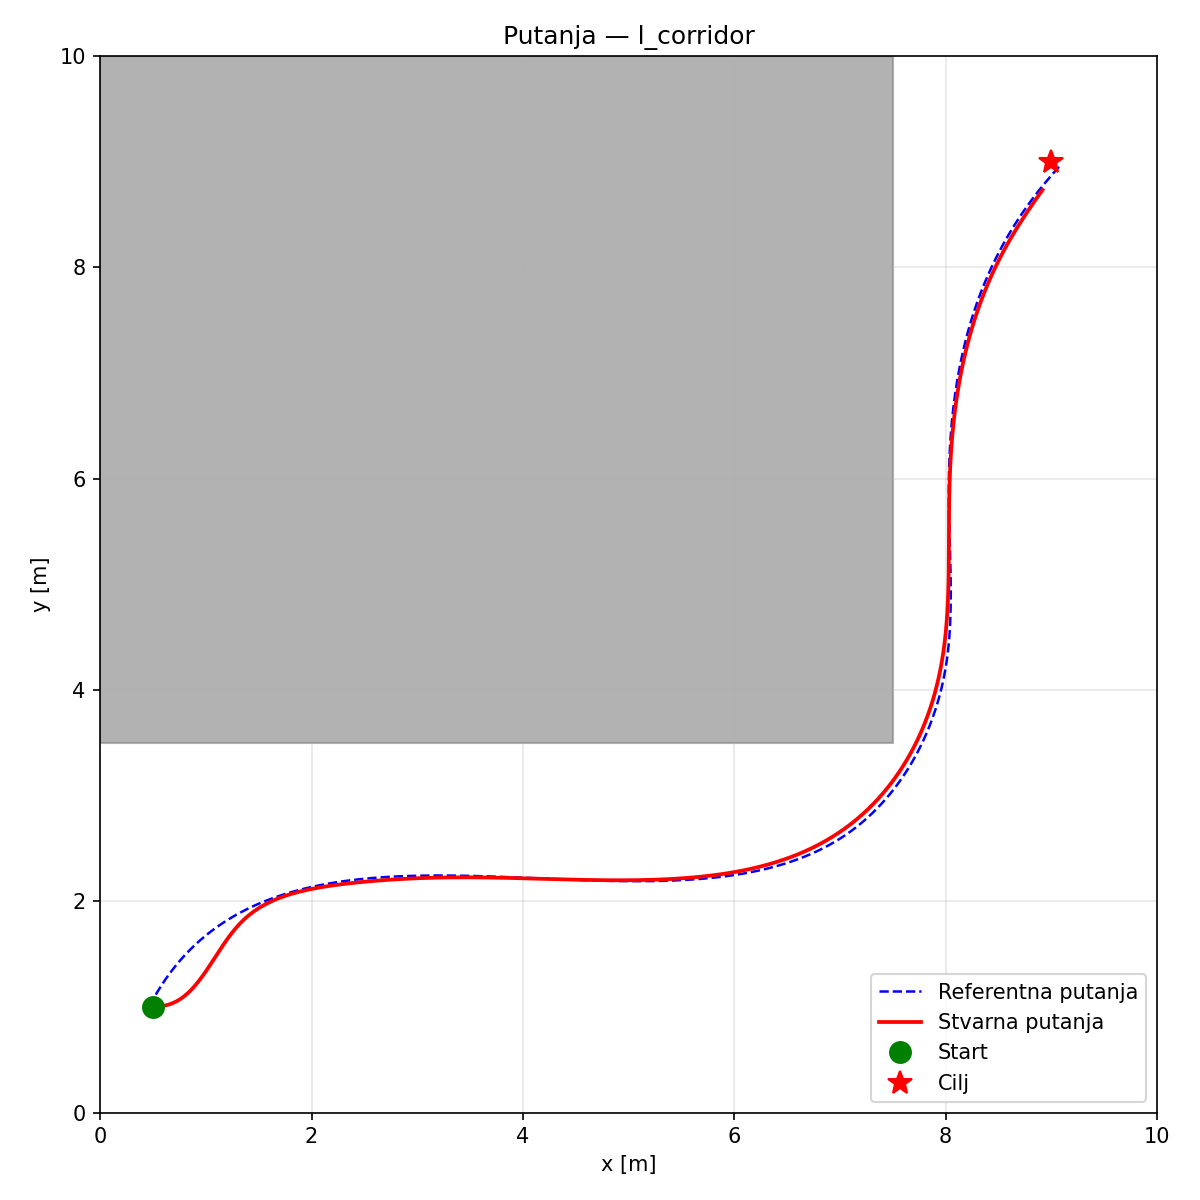
\includegraphics[width=0.82\linewidth]{figures/l_corridor_traj.png}
  \caption{Referentna i stvarna putanja u scenariju L-hodnika. Pravokutna prepreka (siva površina) prisiljava robota na L-oblik putanje.}
  \label{slk:lcorridor_traj}
\end{figure}

\begin{figure}[htbp]
  \centering
  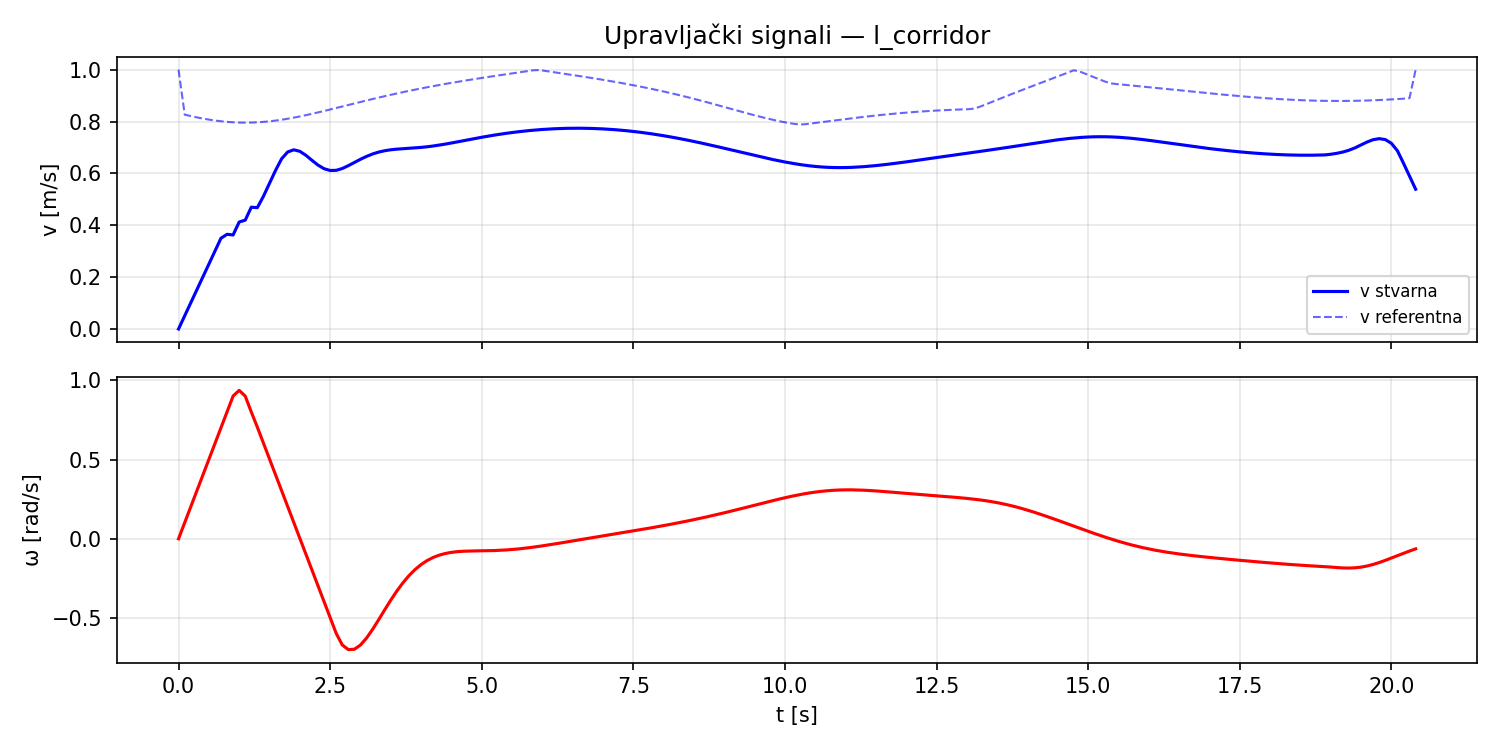
\includegraphics[width=0.82\linewidth]{figures/l_corridor_controls.png}
  \caption{Brzina $v(t)$ i kutna brzina $\omega(t)$ u scenariju L-hodnika. Negativni vrh $\omega \approx -1{,}0$ rad/s oko $t \approx 2{,}8$ s odgovara oštrom zaokretu na kraju horizontalnog dijela.}
  \label{slk:lcorridor_controls}
\end{figure}

Kutna brzina dostiže $\omega_{min} \approx -1{,}0$ rad/s, što je blizu ograničenja $\omega_{max} = 1{,}5$ rad/s i pokazuje da robot mora skrenuti gotovo maksimalnom kutnom brzinom kako bi prošao oštar ugao hodnika.

\begin{figure}[htbp]
  \centering
  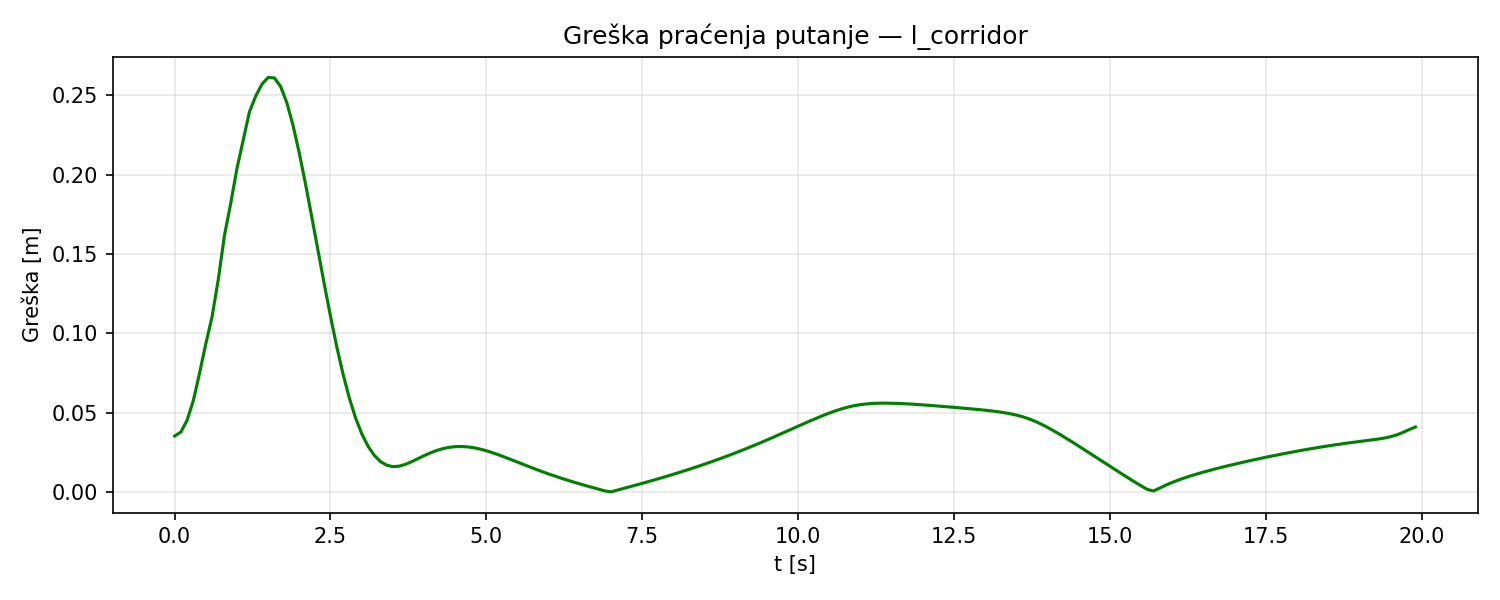
\includegraphics[width=0.82\linewidth]{figures/l_corridor_error.png}
  \caption{Greška praćenja u scenariju L-hodnika. Inicijalni vrh od $0{,}285$ m najveći je u svim pravilnim scenarijima.}
  \label{slk:lcorridor_error}
\end{figure}

\begin{table}[H]
\centering
\caption{Metrike --- L-hodnik}
\label{tab:lcorridor}
\begin{tabular}{lll}
\toprule
Metrika & Vrijednost & Usporedba s osnovnim \\
\midrule
RMSE & $0{,}0724$ m & $+110{,}2$\% \\
CTE srednji & $0{,}0457$ m & $+328{,}3$\% \\
CTE max & $0{,}2610$ m & $+76{,}6$\% \\
Greška smjera (srednja) & $4{,}90°$ & $+79{,}7$\% \\
Vrijeme do cilja & $20{,}40$ s & $+2{,}0$\% \\
CPU (prosjek / max) & $0{,}103$ ms / $0{,}251$ ms & $+13{,}2$\% \\
Dostigao cilj & Da & --- \\
\bottomrule
\end{tabular}
\end{table}

Najveći inicijalni vrh greške ($0{,}285$ m) nastaje kombinacijom greške pozicije i greške smjera na startu --- robot stoji na $y = 1{,}0$ m s $\theta_0 = 0$, dok referentna putanja odmah skreće prema $y \approx 2{,}2$ m. Bez tog prijelaznog odziva prosječna greška u oba segmenta hodnika bila bi usporediva s jednostavnijim scenarijima.

\FloatBarrier
% ─────────────────────────────────────────────────────────────────────────────
\section{U-oblik}
\label{sec:r_ushape}

Tri pravokutne prepreke formiraju slijepu ulicu otvorenu prema jugu: lijeva stranica, desna stranica i gornja stranica U-oblika. Robot polazi iz $(5{,}0;\; 0{,}5)$ s $\theta_0 = \pi/2$ i mora doseći cilj $(5{,}0;\; 9{,}5)$, koji se nalazi izravno iza gornje stranice U. Naivni pristup prema cilju odveo bi robota ravno u zamku.

Scenarij demonstrira neophodnost dvoslojne arhitekture: A* koji vidi cijeli prostor odjednom pronalazi jedini prohodani put --- zaobilazeći U-oblik izvana s desne strane. NMPC s horizontom $N = 20$ (predikcija $= 2$ s) pak ne može sam zaključiti o topologiji zamke, pa bi bez globalne reference mogao zaglaviti unutar U-oblika.

\begin{figure}[htbp]
  \centering
  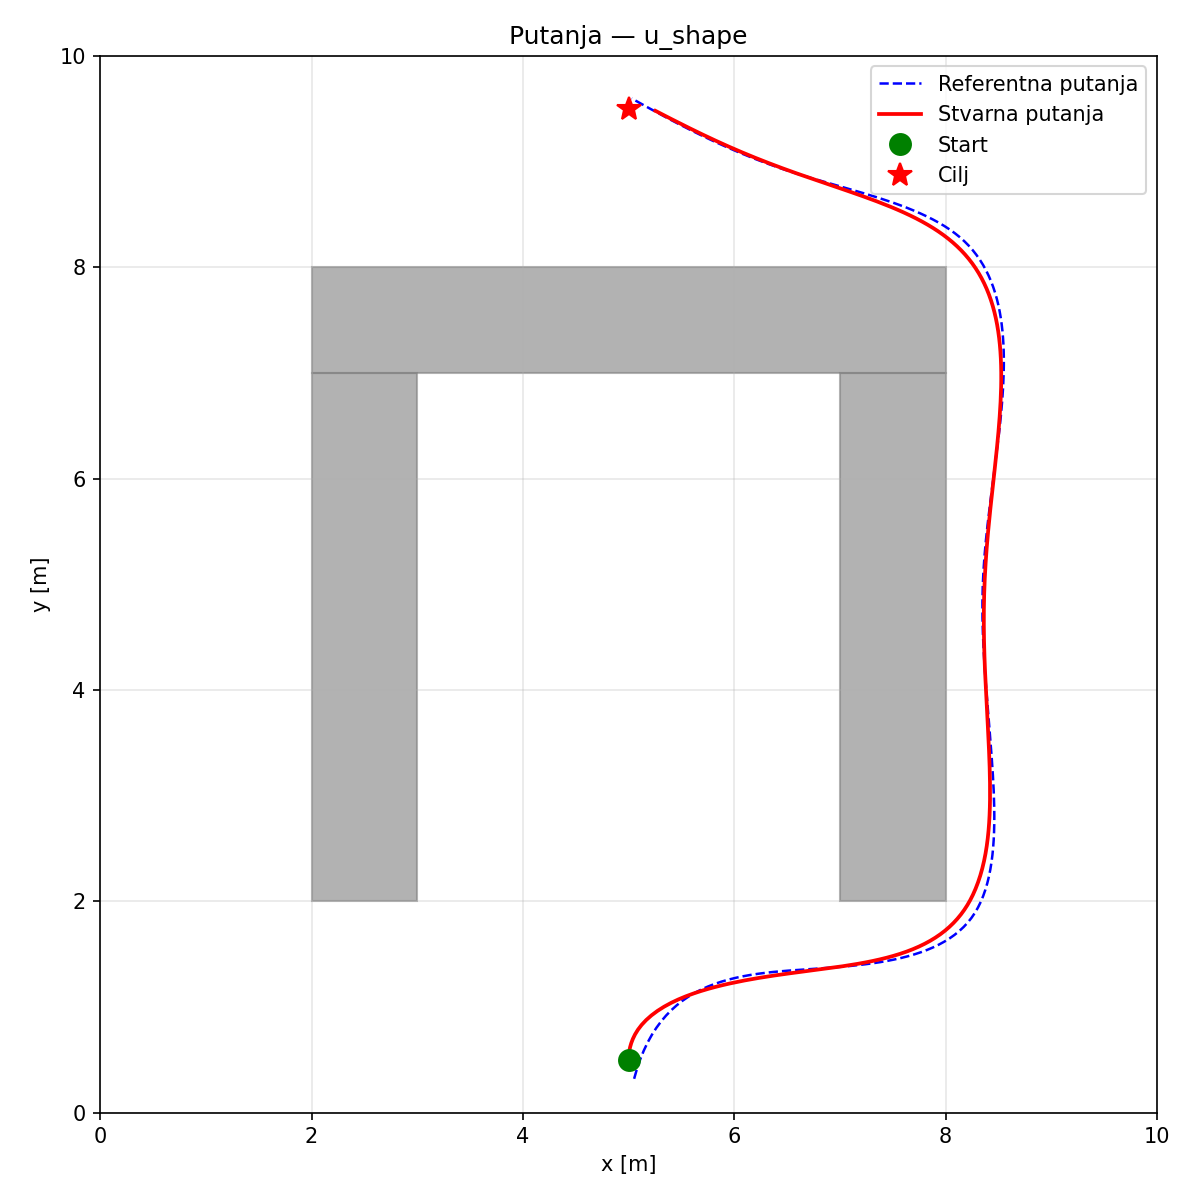
\includegraphics[width=0.82\linewidth]{figures/u_shape_traj.png}
  \caption{Referentna i stvarna putanja u scenariju U-oblika. A* planira put oko desne strane U-oblika, izbjegavajući slijepu ulicu.}
  \label{slk:ushape_traj}
\end{figure}

\begin{figure}[htbp]
  \centering
  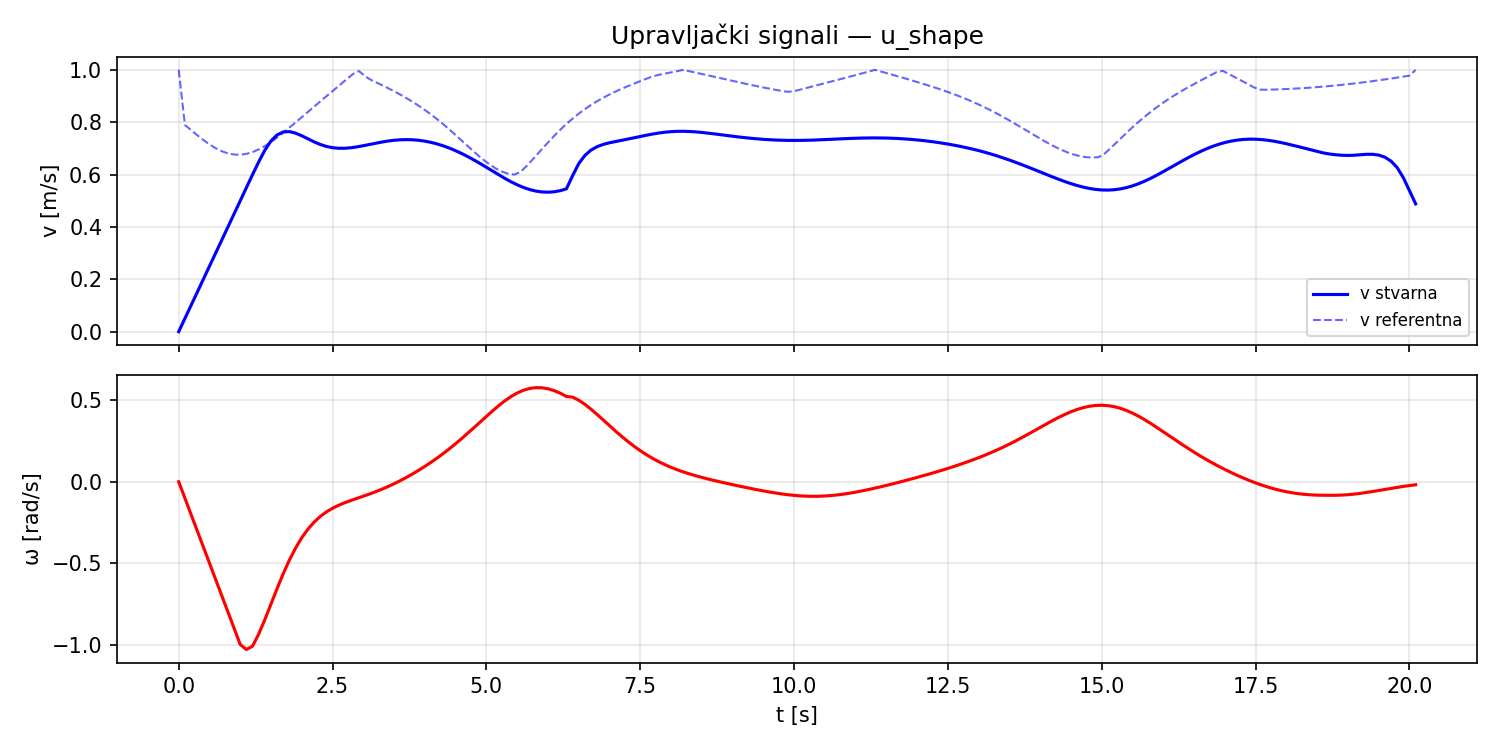
\includegraphics[width=0.82\linewidth]{figures/u_shape_controls.png}
  \caption{Upravljački profili u scenariju U-oblika. Tri vrha $\omega$ odgovaraju trima zavojima na putu oko U-oblika.}
  \label{slk:ushape_controls}
\end{figure}

\begin{figure}[htbp]
  \centering
  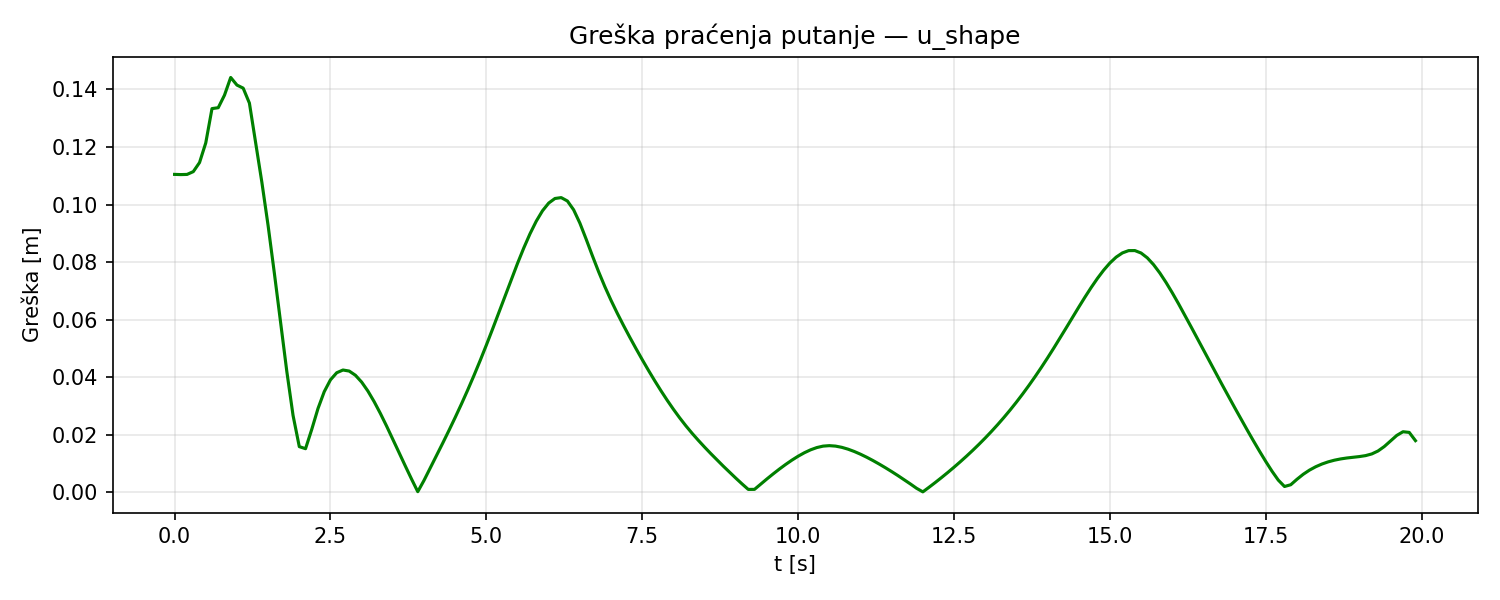
\includegraphics[width=0.82\linewidth]{figures/u_shape_error.png}
  \caption{Greška praćenja u scenariju U-oblika. Tri vrha greške odgovaraju trima zavojima putanje.}
  \label{slk:ushape_error}
\end{figure}

\begin{table}[H]
\centering
\caption{Metrike --- U-oblik}
\label{tab:ushape}
\begin{tabular}{lll}
\toprule
Metrika & Vrijednost & Usporedba s osnovnim \\
\midrule
RMSE & $0{,}0550$ m & $+59{,}8$\% \\
CTE srednji & $0{,}0400$ m & $+274{,}5$\% \\
CTE max & $0{,}1413$ m & $-4{,}4$\% \\
Greška smjera (srednja) & $3{,}19°$ & $+16{,}9$\% \\
Vrijeme do cilja & $20{,}10$ s & $+0{,}5$\% \\
CPU (prosjek / max) & $0{,}114$ ms / $0{,}270$ ms & $+25{,}3$\% \\
Dostigao cilj & Da & --- \\
\bottomrule
\end{tabular}
\end{table}

Uspješno dovršavanje ovog scenarija potvrđuje ispravnost dvoslojne arhitekture. RMSE od $55{,}0$ mm drugi je po redu (iza L-hodnika) jer svaki od tri zavoja nakratko podigne grešku, no između zavoja praćenje je na razini osnovnog scenarija.

\FloatBarrier
% ─────────────────────────────────────────────────────────────────────────────
\section{Poremećaj i oporavak}
\label{sec:r_perturbation}

Scenarij ispituje sposobnost oporavka sustava od nagle vanjske sile. Konfiguracija je identična osnovnom scenariju (ravna putanja od $(0{,}5;\; 5{,}0)$ do $(9{,}5;\; 5{,}0)$), s tom razlikom da se u koraku $k = 30$ ($t = 3{,}0$ s) stanje robota pomakne za $\Delta y = +1{,}0$ m. Poremećaj modelira nagli udarac --- događaj koji sustav ne može predvidjeti jer nije dio modela.

\begin{figure}[htbp]
  \centering
  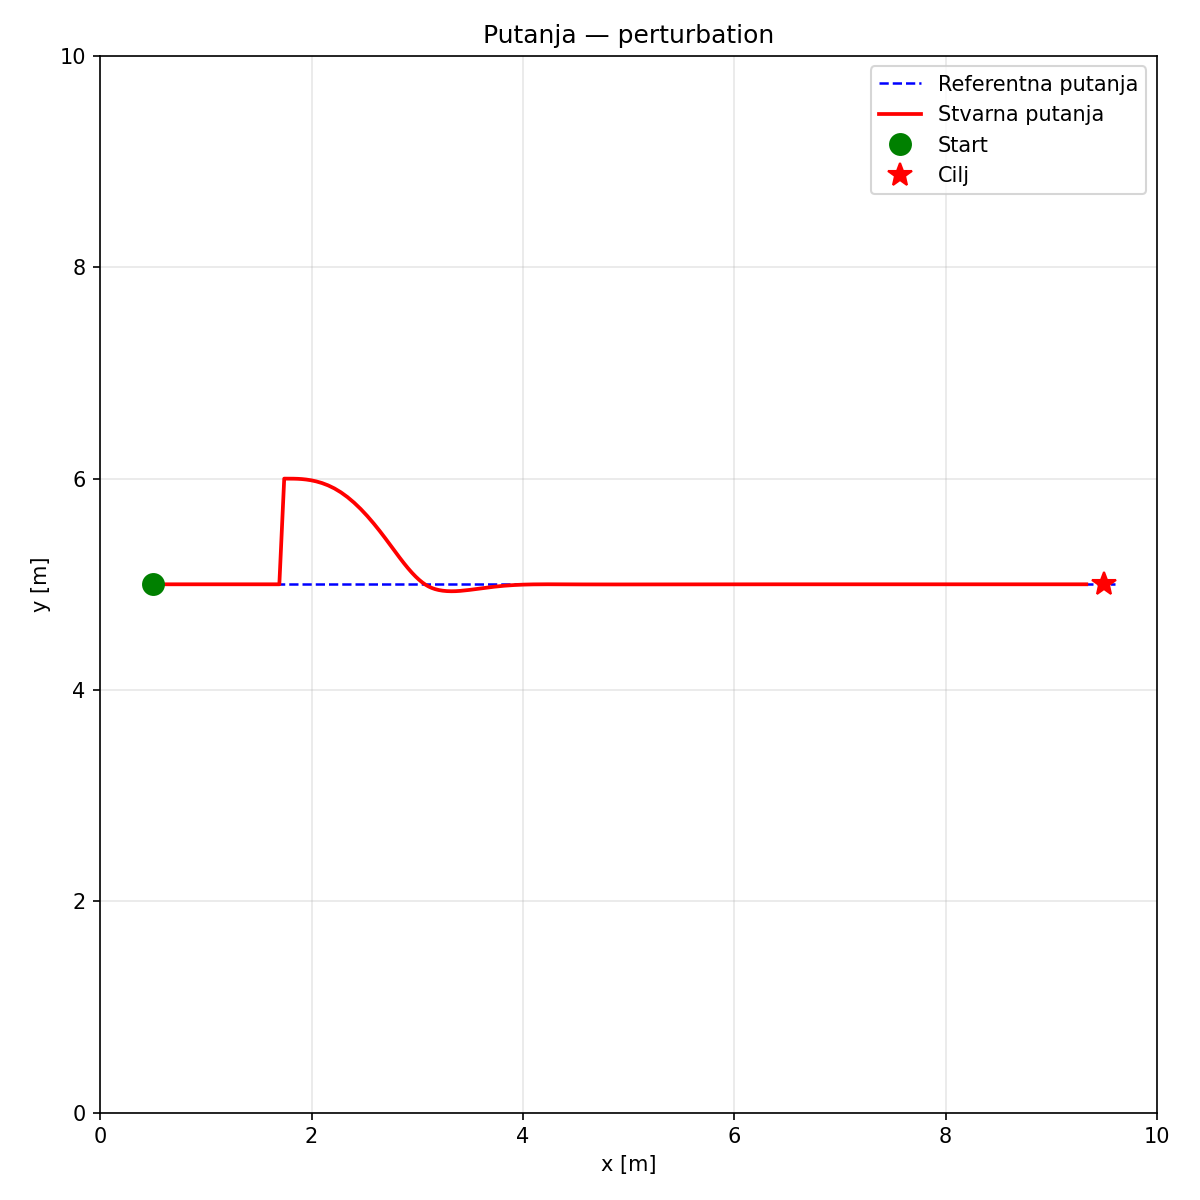
\includegraphics[width=0.82\linewidth]{figures/perturbation_traj.png}
  \caption{Referentna i stvarna putanja u scenariju s poremećajem. Nagli pomak za $1{,}0$ m vidljiv je kao karakteristični skok u trajektoriji, nakon kojega robot brzo vraća na referentnu putanju.}
  \label{slk:perturbation_traj}
\end{figure}

Do $t = 3{,}0$ s robot savršeno prati horizontalnu referencu. U trenutku poremećaja robot je transliran na $y \approx 6{,}0$ m. NMPC u sljedećem koraku prima stvarno stanje, vidi grešku od $1{,}0$ m i počinje ispravljati poziciju robota. Robot opisuje luk koji ga vraća prema referentnoj putanji i već pri $t \approx 5{,}2$ s ponovo se poravnava s referencom.

\begin{figure}[htbp]
  \centering
  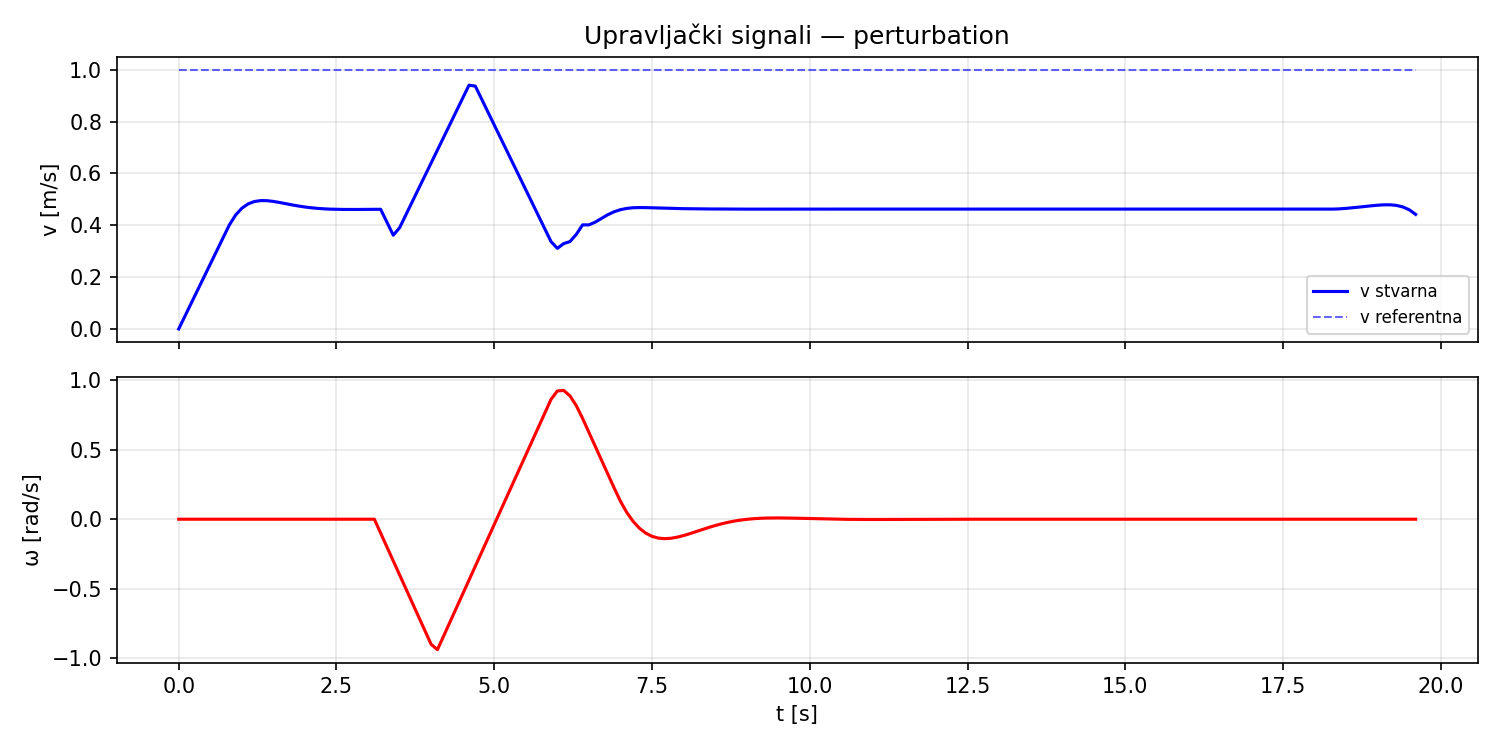
\includegraphics[width=0.82\linewidth]{figures/perturbation_controls.png}
  \caption{Upravljački signali u scenariju s poremećajem. Korektivni impulsi vidljivi su neposredno nakon $t = 3{,}0$ s.}
  \label{slk:perturbation_controls}
\end{figure}

\begin{figure}[htbp]
  \centering
  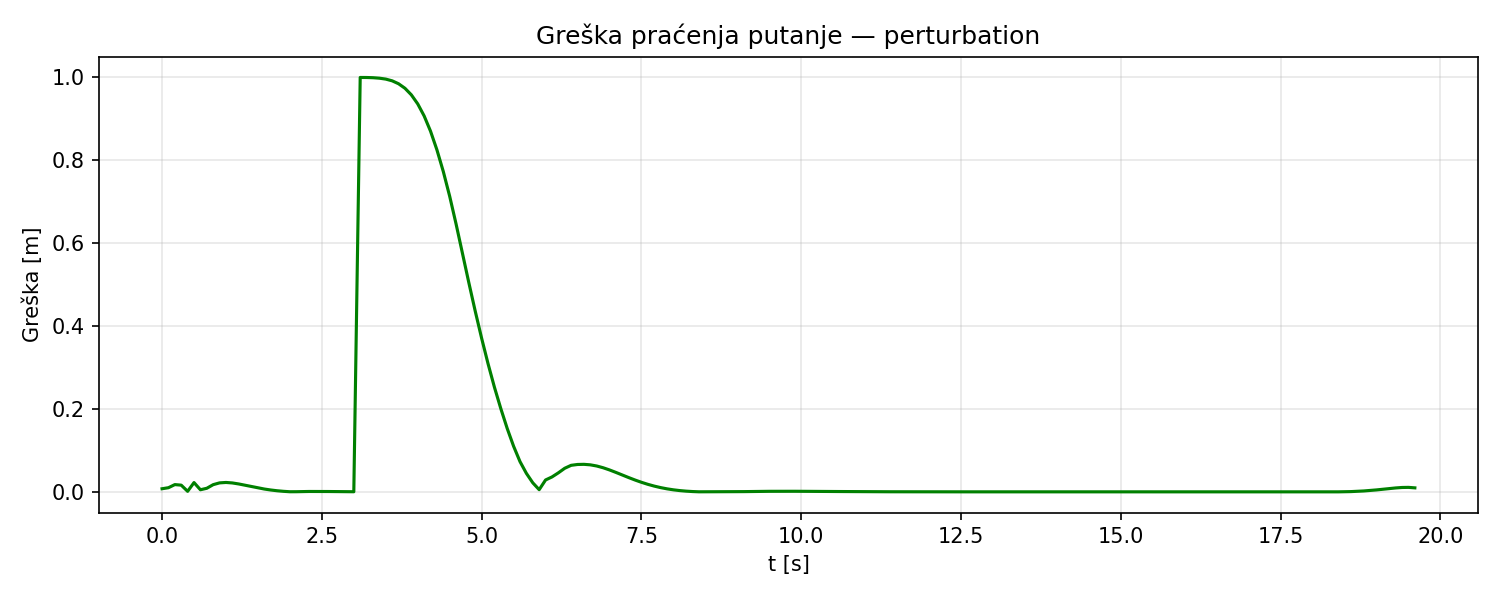
\includegraphics[width=0.82\linewidth]{figures/perturbation_error.png}
  \caption{Greška praćenja u scenariju s poremećajem. CTE skoči na $1{,}0$ m pri $t = 3{,}0$ s i vraća se ispod $0{,}3$ m unutar $22$ koraka ($2{,}2$ s).}
  \label{slk:perturbation_error}
\end{figure}

\begin{table}[H]
\centering
\caption{Metrike --- poremećaj}
\label{tab:perturbation}
\begin{tabular}{ll}
\toprule
Metrika & Vrijednost \\
\midrule
RMSE & $0{,}2736$ m \\
CTE srednji & $0{,}0942$ m \\
CTE max & $1{,}0000$ m \\
Greška smjera (srednja) & $5{,}68°$ \\
Trajanje oporavka (do greške $< 0{,}3$ m) & $22$ koraka ($2{,}2$ s) \\
Vrijeme do cilja & $19{,}60$ s \\
CPU (prosjek / max) & $0{,}118$ ms / $0{,}321$ ms \\
Dostigao cilj & Da \\
\bottomrule
\end{tabular}
\end{table}

Visoki RMSE ($273{,}6$ mm) posljedica je isključivo jednog trenutačnog poremećaja. Ključni zaključak jest da NMPC u zatvorenoj petlji automatski ispravlja poremećaje --- nije implementirana nikakva posebna logika za detekciju ili oporavak. Sustav na svakom koraku prima stvarno stanje i rješava OCP prema naprijed, što samo po sebi generira korektivne akcije.

\FloatBarrier
% ─────────────────────────────────────────────────────────────────────────────
\section{Gusti raspored prepreka}
\label{sec:r_cluttered}

Scenarij smješta sedam kružnih prepreka polumjera $0{,}6$--$0{,}8$ m na različite položaje u prostoru. Robot mora prijeći dijagonalnu putanju od $(0{,}5;\; 0{,}5)$ do $(9{,}5;\; 9{,}5)$. Scenarij testira skalabilnost sustava s povećanim brojem mekih ograničenja prepreka u OCP-u.

\begin{figure}[htbp]
  \centering
  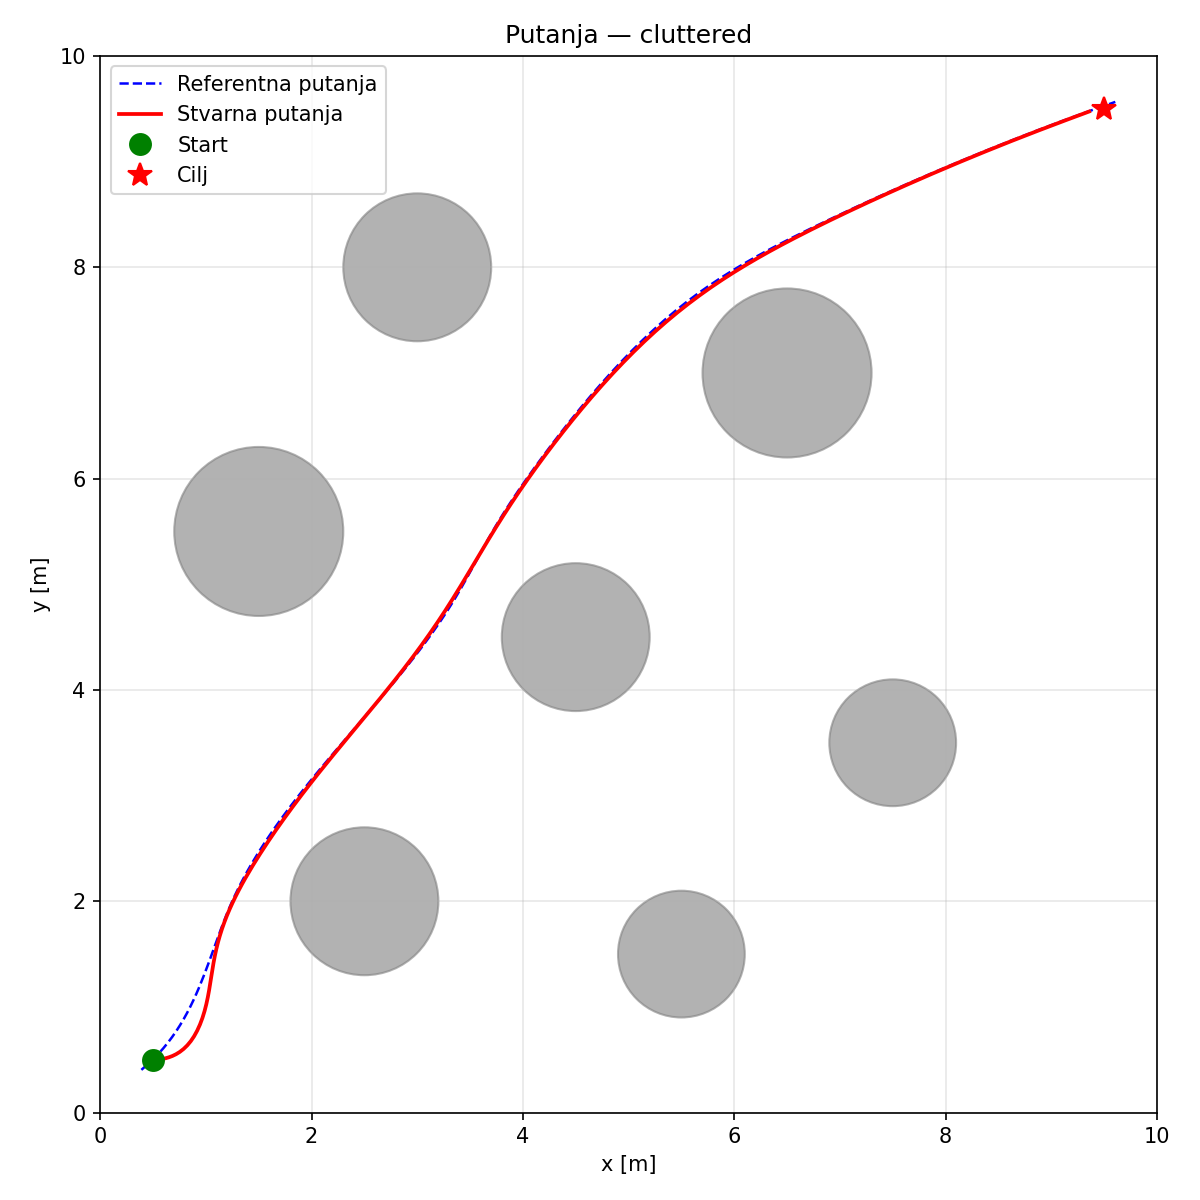
\includegraphics[width=0.82\linewidth]{figures/cluttered_traj.png}
  \caption{Referentna i stvarna putanja u scenariju gustog rasporeda prepreka. A* pronalazi glatku trajektoriju između svih sedam prepreka.}
  \label{slk:cluttered_traj}
\end{figure}

\begin{figure}[htbp]
  \centering
  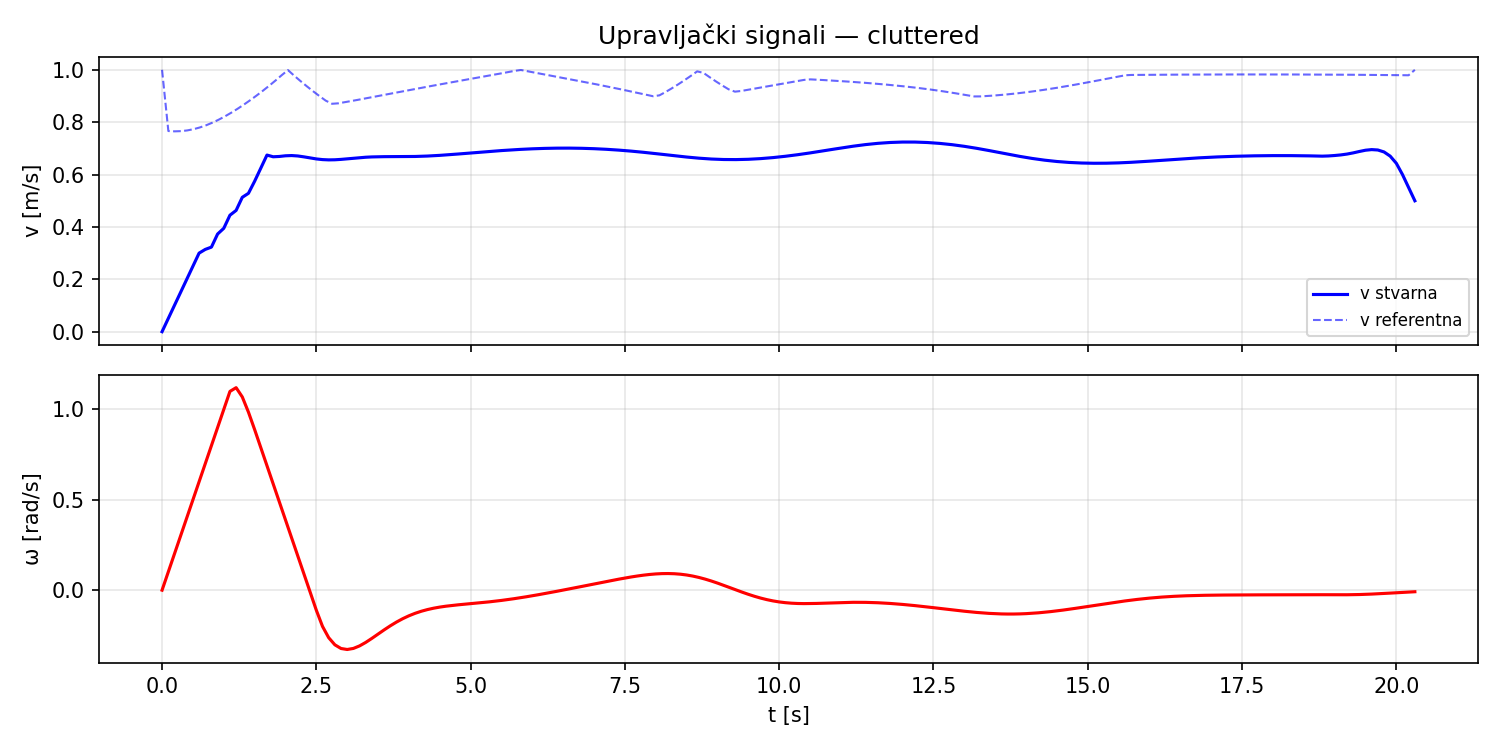
\includegraphics[width=0.82\linewidth]{figures/cluttered_controls.png}
  \caption{Upravljački profili u scenariju gustog rasporeda. Robot dosljedno održava brzinu oko $0{,}65$--$0{,}70$ m/s --- NMPC autonomno bira nižu brzinu pri navigaciji kroz zakrivljenu putanju.}
  \label{slk:cluttered_controls}
\end{figure}

Stvarna brzina dosljedno se zadržava ispod $v_{max} = 1{,}0$ m/s jer NMPC autonomno bira nižu brzinu pri navigaciji kroz zakrivljenu putanju između sedam prepreka.

\begin{figure}[htbp]
  \centering
  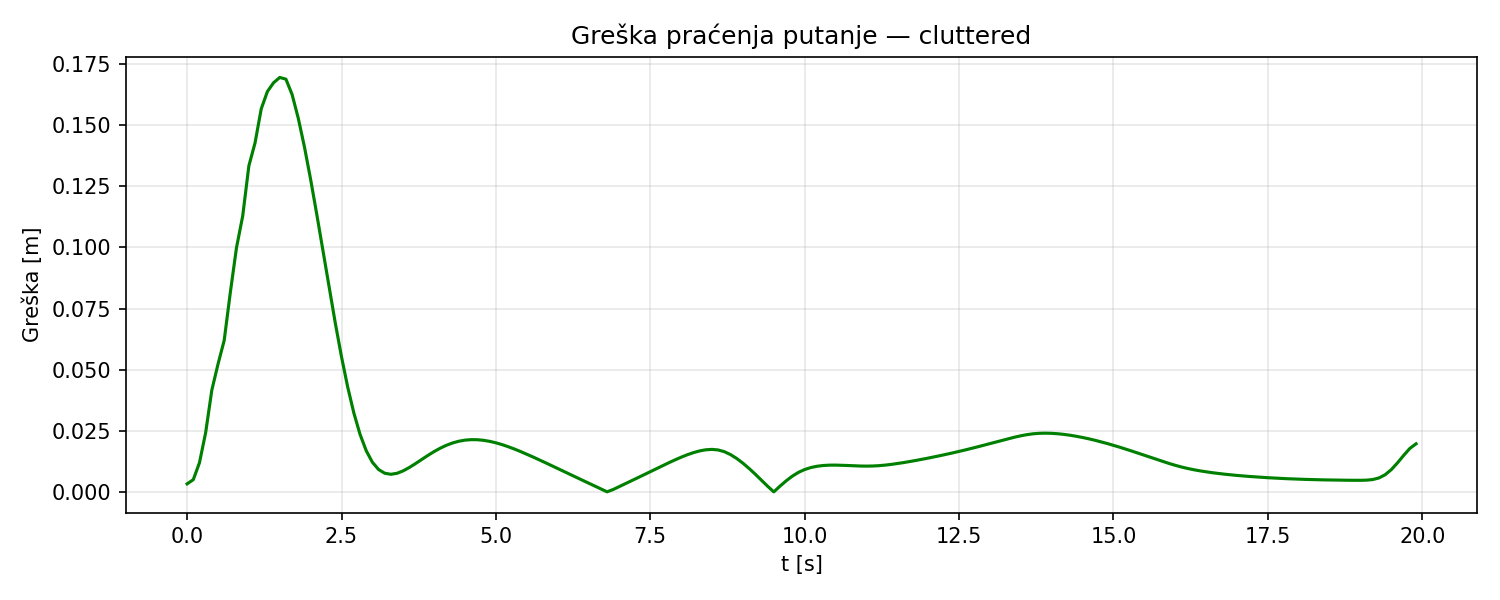
\includegraphics[width=0.82\linewidth]{figures/cluttered_error.png}
  \caption{Greška praćenja u scenariju gustog rasporeda. Nakon inicijalnog vrha, greška ostaje u rasponu $0{,}01$--$0{,}033$ m.}
  \label{slk:cluttered_error}
\end{figure}

\begin{table}[H]
\centering
\caption{Metrike --- gusti raspored prepreka}
\label{tab:cluttered}
\begin{tabular}{lll}
\toprule
Metrika & Vrijednost & Usporedba s osnovnim \\
\midrule
RMSE & $0{,}0429$ m & $+24{,}5$\% \\
CTE srednji & $0{,}0232$ m & $+116{,}9$\% \\
CTE max & $0{,}1678$ m & $+13{,}5$\% \\
Greška smjera (srednja) & $3{,}43°$ & $+25{,}8$\% \\
Broj prepreka & 7 & --- \\
Vrijeme do cilja & $20{,}30$ s & $+1{,}5$\% \\
CPU (prosjek / max) & $0{,}107$ ms / $0{,}277$ ms & $+17{,}6$\% \\
Dostigao cilj & Da & --- \\
\bottomrule
\end{tabular}
\end{table}

RMSE od $42{,}9$ mm je iznimno dobar rezultat za scenarij s najvećim brojem prepreka --- bolji od L-hodnika ($72{,}4$ mm) i U-oblika ($55{,}0$ mm). Razlog je glatka dijagonalna putanja bez naglih zavoja od $90°$. Dodatno CPU opterećenje od $17{,}6$\% u odnosu na osnovni scenarij potvrđuje da dodavanje sedam mekih ograničenja nema značajan utjecaj na računalni teret.

\FloatBarrier
% ─────────────────────────────────────────────────────────────────────────────
\section{Analiza osjetljivosti: predikcijski horizont $N$}
\label{sec:r_horizon}

Predikcijski horizont $N$ temeljni je projektni parametar koji definira broj koraka unaprijed u OCP-u. Duži horizont teorijski omogućuje bolju predikciju, ali povećava dimenzionalnost optimizacijskog problema i time računalni trošak. Analiza je provedena za $N \in \{5,\ 10,\ 15,\ 20,\ 30,\ 40\}$ na scenariju s jednom preprekom.

\begin{figure}[htbp]
  \centering
  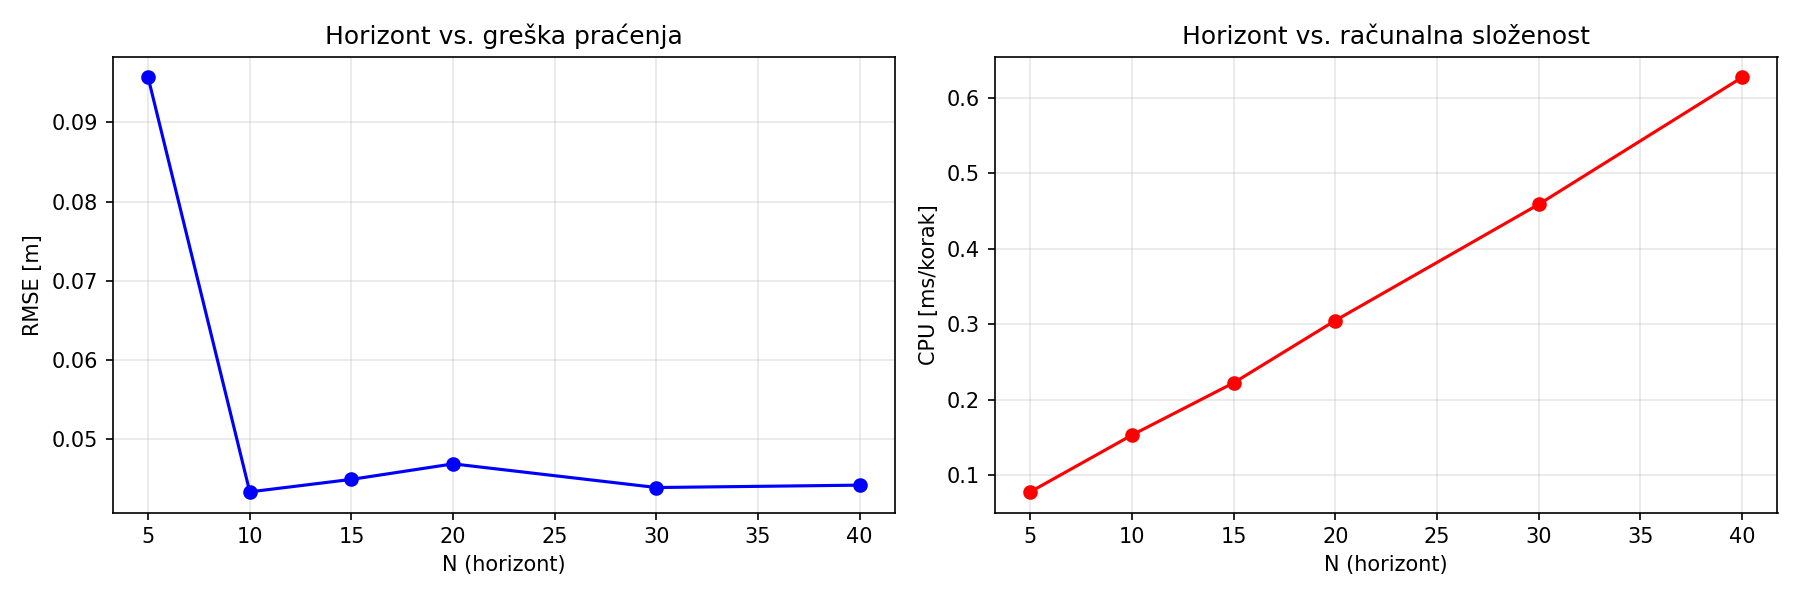
\includegraphics[width=0.95\linewidth]{figures/tuning_horizon.png}
  \caption{Greška praćenja (RMSE) i prosječno CPU vrijeme u ovisnosti o predikcijskom horizontu $N$. Zadana vrijednost $N = 20$ označena je kao referentna.}
  \label{slk:tuning_horizon}
\end{figure}

Rezultati na slici~\ref{slk:tuning_horizon} pokazuju tri zone:
\begin{itemize}
  \item \textbf{Kratki horizont ($N = 5$):} RMSE iznosi $95{,}7$ mm. Kratka predikcija ograničava predviđanje zakrivljene putanje izbjegavanja prepreke.
  \item \textbf{Prijelazna zona ($N = 10$--$20$):} RMSE naglo pada na $43{,}3$ mm pri $N = 10$, a zatim blago oscilira do $46{,}9$ mm pri $N = 20$.
  \item \textbf{Zasićena zona ($N = 30$--$40$):} RMSE se stabilizira na $\approx 44$ mm bez daljnjeg poboljšanja.
\end{itemize}

\begin{table}[H]
\centering
\caption{Kompromis preciznosti i CPU-a za različite horizonte}
\label{tab:horizon}
\begin{tabular}{llll}
\toprule
$N$ & RMSE [mm] & CPU prosjek [ms] & Normalizirani CPU \\
\midrule
5 & $95{,}7$ & $0{,}078$ & $1{,}0\times$ \\
10 & $43{,}3$ & $0{,}153$ & $2{,}0\times$ \\
15 & $44{,}9$ & $0{,}222$ & $2{,}9\times$ \\
\textbf{20} & $\mathbf{46{,}9}$ & $\mathbf{0{,}305}$ & $\mathbf{3{,}9\times}$ \\
30 & $43{,}9$ & $0{,}459$ & $5{,}9\times$ \\
40 & $44{,}2$ & $0{,}627$ & $8{,}1\times$ \\
\bottomrule
\end{tabular}
\end{table}

CPU raste gotovo linearno s $N$, što je konzistentno s teorijskim ponašanjem SQP\_RTI solvera čija složenost po iteraciji raste linearno s dimenzijom predikcijskog vektora. Odabir $N = 20$ temelji se na uravnoteženom kompromisu: u usporedbi s $N = 10$ postiže stabilniji RMSE, a u usporedbi s $N = 30$ razlika u RMSE manja je od $3$ mm uz $33$\% manji CPU.

\textbf{Napomena o metodološkoj razlici CPU vrijednosti.} Vrijednosti CPU-a u tablici~\ref{tab:horizon} ($0{,}078$--$0{,}627$ ms) veće su od vrijednosti u scenariju jedne prepreke (tablica~\ref{tab:one_obstacle}, $0{,}099$ ms za $N=20$) iako je RMSE identičan ($46{,}9$ mm). Razlog je metodološka razlika: analiza horizonta pokrenuta je kao zaseban skript koji za svaki $N$ iznova inicijalizira \texttt{AcadosOcpSolver} i generira novi C kod solvera. Svaka inicijalizacija uključuje hladan start (\textit{cold start}) predikcijskog modela bez prethodno zagrijane JIT/kompajlerske predmemorije. Scenarijska usporedba koristi već kompajlirani solver, čiji su SQP\_RTI pozivi brži zahvaljujući zagrijanju predmemorije instrukacija i podataka. Apsolutne vrijednosti u tablici~\ref{tab:horizon} treba tumačiti kao gornju granicu CPU-a za hladni start pri promjeni konfiguracije, a ne kao radne vrijednosti u normalnom radu.

\FloatBarrier
% ─────────────────────────────────────────────────────────────────────────────
\section{Analiza osjetljivosti: težine troška}
\label{sec:r_weights}

Omjer $Q/R$ temeljni je stupanj slobode koji određuje karakter NMPC-a: visoki $Q$ kažnjava grešku praćenja, visoki $R$ kažnjava agresivne promjene upravljanja. Testirana su četiri konfiguracijska profila uz konstantan $N = 20$:

\begin{figure}[htbp]
  \centering
  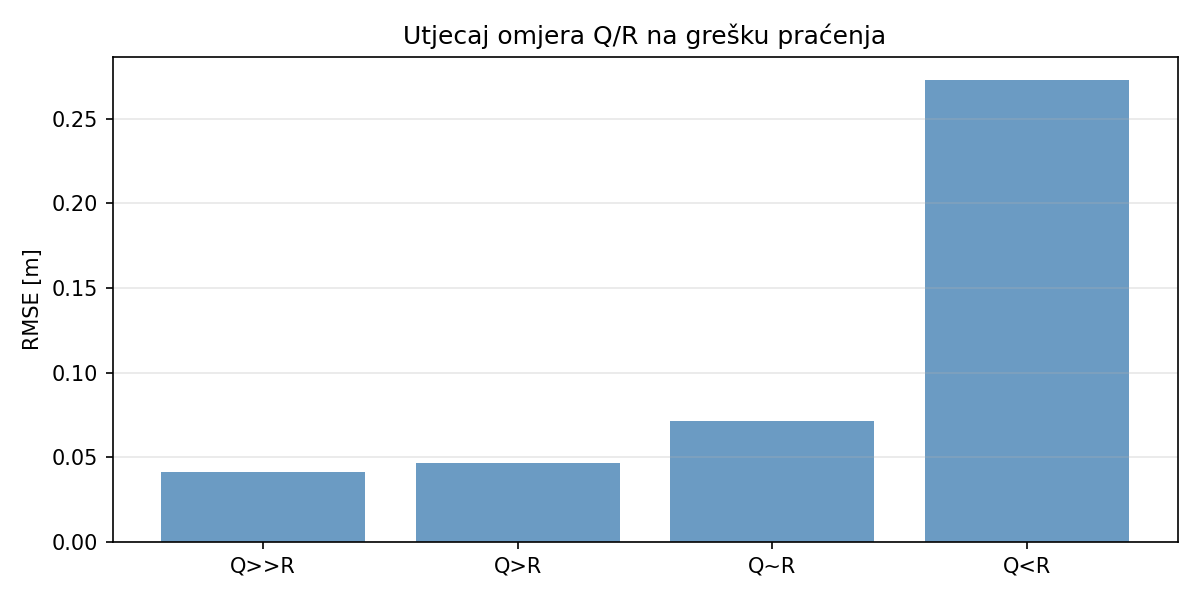
\includegraphics[width=0.82\linewidth]{figures/tuning_weights.png}
  \caption{RMSE praćenja za četiri konfiguracijska profila omjera $Q/R$ u scenariju jedne prepreke.}
  \label{slk:tuning_weights}
\end{figure}

\begin{table}[H]
\centering
\caption{Utjecaj konfiguracije težina na preciznost praćenja}
\label{tab:weights}
\begin{tabular}{lllll}
\toprule
Konfiguracija & $Q$ (pos.) & $R$ & RMSE [mm] & Karakter upravljanja \\
\midrule
Q$\gg$R & $50{,}0$ & $0{,}01$ & $41{,}5$ & Intenzivno, responzivno \\
\textbf{Q$>$R} & $\mathbf{10{,}0}$ & $\mathbf{0{,}1}$ & $\mathbf{46{,}9}$ & \textbf{Glatko, responzivno} \\
Q$\sim$R & $5{,}0$ & $1{,}0$ & $71{,}2$ & Slabije praćenje \\
Q$<$R & $1{,}0$ & $5{,}0$ & $272{,}9$ & Pasivno, neučinkovito \\
\bottomrule
\end{tabular}
\end{table}

Rezultati pokazuju monoton redoslijed: preciznost praćenja raste s porastom omjera $Q/R$. Konfiguracija Q$\gg$R postiže najmanji RMSE ($41{,}5$ mm), no po cijenu agresivnijih upravljačkih akcija. Konfiguracija Q$<$R ($Q = 1{,}0$, $R = 5{,}0$) postiže daleko najlošiji RMSE ($272{,}9$ mm) jer optimizator ``bira'' manje upravljačkih akcija kako bi smanjio trošak $R$, što rezultira trajnom velikom greškom pozicije.

Zadana konfiguracija $Q = 10{,}0$, $R = 0{,}1$ (omjer $100{:}1$) odabrana je kao optimalno kompromisno rješenje koje postiže RMSE od $46{,}9$ mm uz upravljačke signale dovoljno glatke za mehanički sustav.

\FloatBarrier
% ─────────────────────────────────────────────────────────────────────────────
\section{Zbirna usporedba scenarija}
\label{sec:r_summary}

Tablica~\ref{tab:summary} donosi objedinjeni pregled svih sedam testnih scenarija.

\begin{table}[H]
\centering
\caption{Zbirna tablica rezultata --- svi scenariji}
\label{tab:summary}
\small
\begin{tabular}{lllllll}
\toprule
Scenarij & RMSE [m] & CTE sred.\ [m] & Kut.\ greška [°] & Vrij.\ [s] & CPU prs.\ [ms] & Cilj \\
\midrule
Osnovna putanja   & $0{,}0344$ & $0{,}0107$ & $2{,}73$ & $20{,}0$ & $0{,}091$ & Da \\
Jedna prepreka    & $0{,}0469$ & $0{,}0278$ & $3{,}87$ & $20{,}0$ & $0{,}099$ & Da \\
Uski prolaz       & $0{,}0344$ & $0{,}0270$ & $1{,}59$ & $19{,}7$ & $0{,}089$ & Da \\
L-hodnik          & $0{,}0724$ & $0{,}0457$ & $4{,}90$ & $20{,}4$ & $0{,}103$ & Da \\
U-oblik           & $0{,}0550$ & $0{,}0400$ & $3{,}19$ & $20{,}1$ & $0{,}114$ & Da \\
Poremećaj         & $0{,}2736$ & $0{,}0942$ & $5{,}68$ & $19{,}6$ & $0{,}118$ & Da \\
Gusti raspored    & $0{,}0429$ & $0{,}0232$ & $3{,}43$ & $20{,}3$ & $0{,}107$ & Da \\
\bottomrule
\end{tabular}
\end{table}

Svi scenariji završavaju uspješnim dosezanjem cilja. Isključivanjem scenarija poremećaja, RMSE ostalih scenarija kreće se u rasponu od $34{,}4$ mm do $72{,}4$ mm (faktor $2{,}1\times$), što je izvrsna preciznost za sustav koji se kreće brzinom do $1$ m/s.

Prosječno CPU vrijeme iznosi između $0{,}089$ ms i $0{,}118$ ms, a maksimalni izmjereni korak traje $0{,}359$ ms --- što je oko $280\times$ brže od raspoloživog uzornog intervala od $100$ ms. Ovo eksperimentalno potvrđuje da je sustav primjenjiv u stvarnom vremenu i na hardveru s ograničenim procesorskim resursima. Budući da acados generira optimizirani C kod namijenjen ugradbenim sustavima, opravdano je očekivati prihvatljivo vrijeme izvođenja i na slabijem hardveru poput Raspberry Pi 4 --- no to nije eksperimentalno verificirano u ovom radu i ostavlja se za budući rad (poglavlje~\ref{pog:zakljucak}).


\FloatBarrier
% ─────────────────────────────────────────────────────────────────────────────
\section{Nedostižni cilj --- granice sustava}
\label{sec:r_blocked}

Scenarij \texttt{blocked} ispituje ponašanje sustava kada A* algoritam za planiranje putanje ne može pronaći putanju bez sudara s preprekama. Pet kružnih prepreka polumjera $1{,}5$ m postavljeno je u vertikalni niz duž $x = 5{,}0$ m, formirajući potpunu prepreku od $y = 0$ do $y = 10$ m.

Efektivni polumjer svake prepreke pri A* pretraživanju iznosi $r + d_{inf} = 1{,}5 + 0{,}4 = 1{,}9$ m. Razmak između susjednih centara od $2{,}5$ m manji je od $2 \times 1{,}9 = 3{,}8$ m, pa se inflirana područja potpuno preklapaju i formiraju neprobojni zid.

\begin{figure}[H]
  \centering
  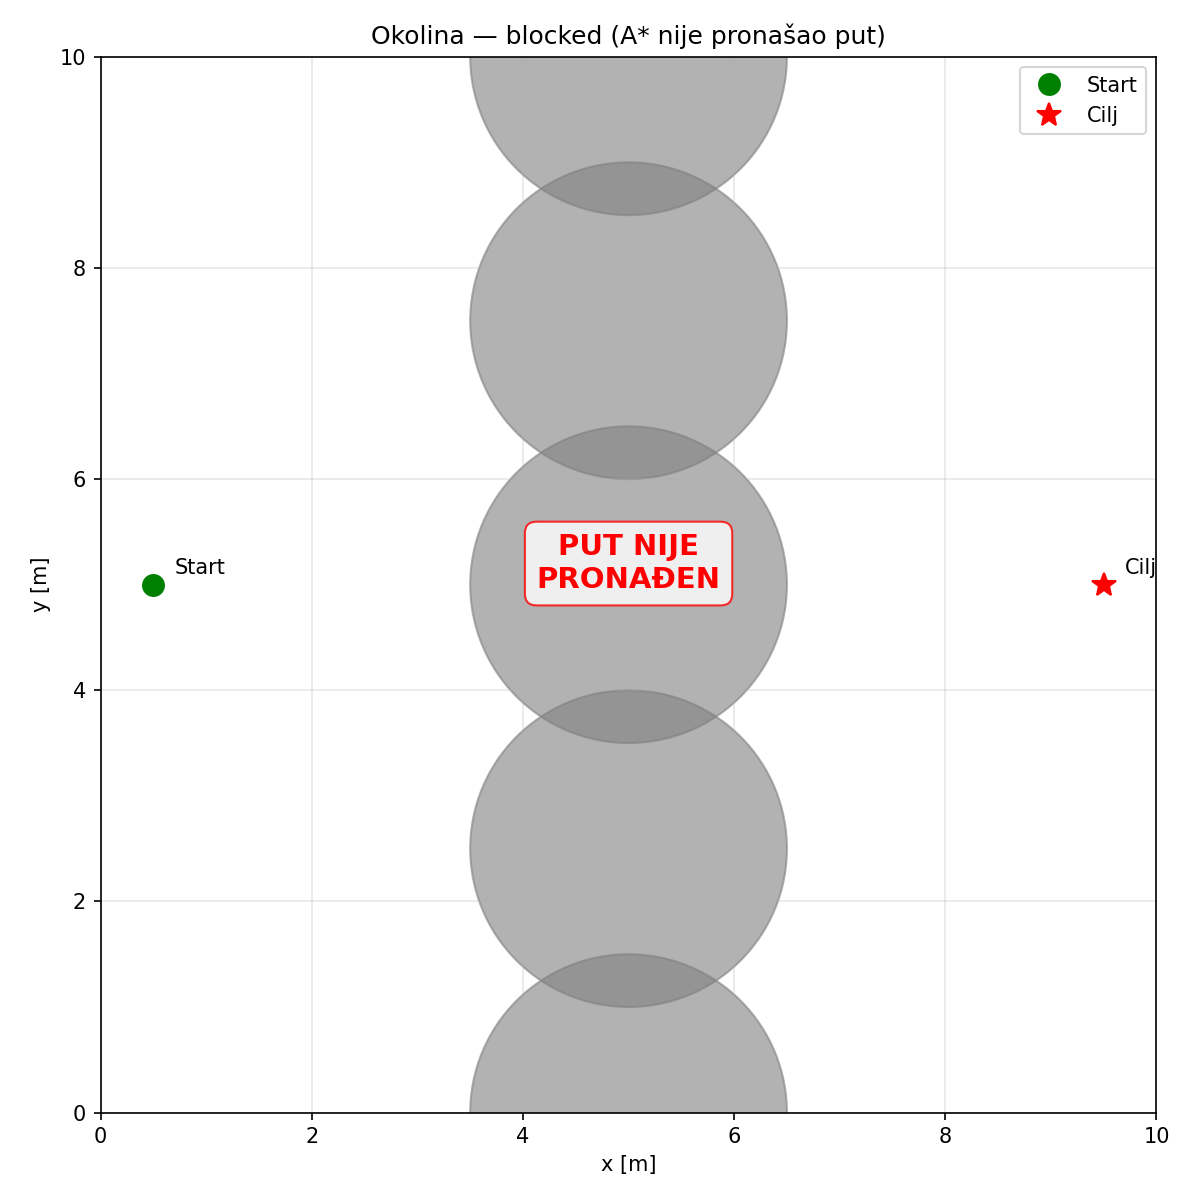
\includegraphics[width=0.82\linewidth]{figures/blocked_env.png}
  \caption{Vizualizacija blokirane okoline. Pet kružnih prepreka formira vertikalni zid koji potpuno blokira putanju od starta (lijevo) do cilja (desno).}
  \label{slk:blocked_env}
\end{figure}

A* ne pronalazi put i ispravno detektira neizvedivost --- heuristika ga vodi sve dok ne iscrpi sve dostupne čvorove na strani starta:

\begin{listing}[H]
\begin{minted}{bash}
RuntimeError: A*: nema puta od starta do cilja
\end{minted}
\caption{Poruka sustava pri nedostižnom cilju}
\end{listing}

Budući da referentna putanja nije generirana, NMPC solver se uopće ne pokreće. Ovo je ispravno ponašanje: A* algoritam djeluje kao \emph{filter izvedivosti} koji detektira neriješivost na razini planiranja, što je računalno učinkovito i arhitekturno ispravno.


% !TEX root = ../zavrsni_rad.tex

\chapter{Zaključak}
\label{pog:zakljucak}

\section{Pregled postignutih rezultata}

U ovom radu razvijen je dvoslojni sustav za planiranje i praćenje putanje mobilnog robota u poznatom statičkom prostoru. Globalni sloj temelji se na A* algoritmu koji pretražuje diskretiziranu mrežu rezolucije $0{,}2$ m uz ukupnu inflaciju prepreka $0{,}4$ m, a dobivena putanja se izglađuje uz vizualizacijski profil brzine prilagođen zakrivljenosti. Lokalni sloj koristi NMPC regulator s proširenim modelom monocikla i SQP\_RTI solverom koji na svakom uzorkovnom koraku od $\Delta t = 0{,}1$ s rješava OCP s horizontom $N = 20$ koraka.

Sustav je testiran na sedam scenarija koji pokrivaju spektar od jednostavne ravne putanje do gusto popunjene okoline i namjerno zadanog poremećaja stanja. Svi scenariji završili su uspješnim dosezanjem cilja, s RMSE od $34{,}4$ do $72{,}4$ mm u statičkim scenarijima i prosječnim CPU vremenom od $0{,}089$ do $0{,}118$ ms po koraku.

\section{Analiza ključnih nalaza}

\subsection*{Preciznost praćenja i utjecaj geometrije okoline}

Rezultati pokazuju da preciznost praćenja nije monotono određena brojem prepreka, nego geometrijom putanje koju prepreke nameću. Scenarij s jednom preprekom (RMSE $= 46{,}9$ mm) postiže lošiji rezultat od gustog rasporeda sedam prepreka (RMSE $= 42{,}9$ mm), jer raspoređene prepreke u potonjem slučaju dopuštaju glatku dijagonalnu trajektoriju, dok jedna prepreka u nepovoljnom položaju prisiljava na oštriji zaokret. Scenariji s hodnicima (L-hodnik, U-oblik) s RMSE od $72{,}4$ mm i $55{,}0$ mm postavljaju najveći zahtjev jer oblik hodnika nameće skretanja blizu $90°$.

\subsection*{Automatski oporavak od poremećaja}

Scenarij perturbacije pokazuje prednost MPC arhitekture: oporavak od poremećaja nije posebno kodiran, već je prirodna posljedica zatvorene optimizacijske petlje. Nagli pomak od $\Delta y = 1{,}0$ m kompenziran je unutar $2{,}2$ s ($22$ koraka) bez ikakvih modifikacija sustava. Sustav na svakom koraku prima stvarno stanje i rješava OCP prema naprijed, pa automatski ispravlja grešku bez posebne logike za oporavak.

\subsection*{Računalna provedivost}

Prosječno CPU vrijeme kreće se od $0{,}089$ do $0{,}118$ ms po koraku, što je daleko ispod uzornog intervala od $100$ ms. Zanimljiv nalaz je da CPU prosjek ne ovisi izravno o broju prepreka: scenarij poremećaja bez prepreka postiže najviši prosjek ($0{,}118$ ms) zbog intenzivnih korektivnih iteracija, dok gusti raspored sedam prepreka iznosi $0{,}107$ ms. Topologija putanje i dinamika stanja imaju veći utjecaj na računalni teret od broja mekih ograničenja.

\subsection*{Analiza osjetljivosti parametara}

Analiza horizonta $N$ otkriva zasićenje preciznosti za $N \geq 10$ (RMSE $\approx 43$--$47$ mm), dok CPU raste gotovo linearno. Odabrani $N = 20$ ($0{,}305$ ms/korak) postiže $33$\% manji CPU od $N = 30$ uz manje od $3$ mm razlike u RMSE. Analiza težina $Q/R$ pokazuje da što je $Q$ veći u odnosu na $R$, robot preciznije prati putanju. Konfiguracija Q$<$R rezultira najlošijim RMSE ($272{,}9$ mm) jer robot tada više kažnjava agresivno skretanje nego grešku pozicije.

\section{Ograničenja implementiranog sustava}

Implementirani sustav počiva na nekoliko pretpostavki koje ograničavaju izravnu primjenjivost u stvarnim scenarijima:

\textbf{Poznata i statička okolina.} A* algoritam zahtijeva potpunu kartu okoline unaprijed. U dinamičkim okolinama s pokretnim preprekama potrebna je integracija senzorskog sustava i reaktivno replaniranje.

\textbf{Kinematički model bez dinamike.} Model monocikla zanemaruje inerciju i trenje kotača. Na visokim brzinama ili klizavim podlogama ova aproksimacija nije valjana i zahtijeva dinamički model.

\textbf{Kružne prepreke.} Implementirana ograničenja prepreka pretpostavljaju kružni oblik. Prepreke proizvoljnog oblika zahtijevaju konveksnu aproksimaciju poligona ili pristup temeljen na polju predznačenih udaljenosti (SDF).

\textbf{Simulacijsko okruženje i identičan model.} Svi rezultati dobiveni su u simulaciji. Dodatno, NMPC predikcijski model i model koji simulira stvarnog robota su identični --- oba koriste isti kinematički model monocikla. Zbog toga NMPC "zna" točno kako će se robot ponašati, što daje gornju granicu preciznosti: izmjerene greške praćenja predstavljaju optimistični scenarij koji se na stvarnom robotu ne može dosegnuti. Na stvarnom hardveru prisutni su šum senzora, kašnjenje aktuatora i trenje koje uzrokuju odstupanje od predikcijskog modela, pa je stvarna preciznost praćenja nešto lošija.

\section{Smjernice za buduća istraživanja}

Na temelju postignutih rezultata i identificiranih ograničenja, predlažu se sljedeće smjernice za daljnji razvoj:

\begin{enumerate}
  \item \textbf{Dinamičke prepreke i reaktivno replaniranje:} implementacija A* ponovnog planiranja putanje u stvarnom vremenu pri detekciji novih prepreka
  \item \textbf{Dinamički model robota:} uključivanje inercije i trenja u model kako bi simulacija bila bliža stvarnom ponašanju robota
  \item \textbf{Contouring MPC:} varijanta NMPC-a koja kažnjava bočno odstupanje i brzinu napredovanja po putanji umjesto praćenja diskretnih referentnih točaka
  \item \textbf{Adaptivno podešavanje:} automatsko prilagođavanje težina $Q$ i $R$ ovisno o trenutnoj situaciji, npr.\ agresivnije u zavojima i glađe na ravnom dijelu putanje
  \item \textbf{Testiranje na stvarnom hardveru:} pokretanje sustava na Raspberry Pi ili sličnom računalu kako bi se potvrdilo da radi dovoljno brzo u stvarnim uvjetima; pri tome bi trebalo implementirati i transformaciju $(v, \omega) \to (v_L, v_R)$ opisanu u odjeljku~\ref{sec:diff_drive} za naredbu motornim kontrolerima diferencijalnog robota
\end{enumerate}

\section{Završna ocjena}

Kombinacija A* algoritma i NMPC-a pokazala se kao dobro rješenje za navigaciju mobilnog robota --- sustav precizno prati putanju, automatski se oporavlja od poremećaja i radi unutar zahtjeva intervala uzorkovanja od 100 ms s rezervom od dva reda veličine. Za razliku od jednostavnijih regulatora koji reagiraju tek nakon što se greška dogodi, NMPC gleda unaprijed i pokušava spriječiti grešku dok se još može.

Alat acados znatno pojednostavljuje implementaciju jer automatski generira efikasan solver iz zadane OCP formulacije, što oslobađa korisnika ručnog izvođenja derivacija i pisanja vlastitog solvera. 


%--- LITERATURA ------------------------------------------

\bibliography{literatura}


%--- IZJAVA O UI -------------------------------------------

\begin{izjavaoui}

Tijekom izrade ovog završnog rada korišten je generativni AI alat Claude (Anthropic, verzija Claude Sonnet). Alat je korišten kao pomoć pri programiranju (debugiranje Python koda i konfiguracija acados solvera), istraživanju i razumijevanju literature te razumijevanju matematičkih pojmova vezanih uz NMPC i numeričku optimizaciju.

\paragraph{Osvrt na korištenje umjetne inteligencije:}
Implementacija algoritama (A*, NMPC formulacija u acadosu), odabir metodologije, provedba eksperimenata i interpretacija rezultata rezultat su mog samostalnog rada. Sve tvrdnje, matematičke izvode i zaključke provjerio sam na primarnim izvorima i provjerio kroz simulaciju.
\paragraph{Izjava o korištenju umjetne inteligencije:}
Potvrđujem da sam tijekom izrade ovog završnog rada koristio umjetnu inteligenciju u skladu s Politikom primjerenog korištenja umjetne inteligencije na Fakultetu elektrotehnike i računarstva, te da umjetna inteligencija nije zamijenila moje kritičko razmišljanje niti moj doprinos.

\end{izjavaoui}


%--- SAŽETAK ---------------------------------------------

\begin{sazetak}
U radu je razvijen sustav za navigaciju mobilnog robota koji se kreće od zadane početne točke do cilja izbjegavajući prepreke. Sustav se sastoji od dva dijela: A* algoritma koji pronalazi slobodan put na mreži i NMPC regulatora koji taj put prati u stvarnom vremenu. Robot je modeliran kao monocikl, a putanja se izglađuje kako bi kretanje bilo glatko. NMPC u svakom koraku optimizira kretanje robota uzimajući u obzir ograničenja brzine i prepreke u okolini. Za implementaciju je korišten alat acados koji automatski generira optimizirani kod solvera. Sustav je testiran na sedam scenarija različite složenosti --- od ravne putanje bez prepreka do gustog rasporeda sedam kružnih prepreka i scenarija s naglim bočnim guranjem robota. Svi scenariji završili su dosezanjem cilja. RMSE praćenja u statičkim scenarijima iznosi $34{,}4$--$72{,}4$ mm; u scenariju s perturbacijom ($\Delta y = 1{,}0$ m) RMSE iznosi $273{,}6$ mm, a robot se vraća na referencu unutar $2{,}2$ s. Prosječno vrijeme izračuna po koraku iznosi $0{,}089$--$0{,}118$ ms.
\end{sazetak}

\begin{kljucnerijeci}
  mobilni robot; NMPC; planiranje putanje; acados; SQP\_RTI; A* algoritam; monocikl
\end{kljucnerijeci}

\begin{abstract}
This thesis presents a navigation system for a mobile robot that moves from a start position to a goal while avoiding obstacles. The system consists of two parts: an A* algorithm that finds a free path on a grid, and an NMPC controller that follows the path in real time. The robot is modelled as a unicycle and the path is smoothed to ensure fluid motion. At each step, the NMPC optimises the robot's movement while respecting speed limits and obstacle constraints. The implementation uses the acados framework, which automatically generates optimised solver code. The system was tested on seven scenarios of varying difficulty --- from a straight path with no obstacles to a cluttered environment with seven circular obstacles and a scenario with a sudden lateral push. All scenarios ended with the robot successfully reaching the goal. Path tracking RMSE in static scenarios ranges from $34.4$ to $72.4$ mm; in the perturbation scenario, where a $1.0$ m lateral push is applied, RMSE reaches $273.6$ mm with full recovery within $2.2$ s. Average computation time per step is $0.089$--$0.118$ ms.
\end{abstract}

\begin{keywords}
  mobile robot; NMPC; path planning; acados; SQP\_RTI; A* algorithm; unicycle
\end{keywords}

\end{document}